\documentclass[twoside]{book}

% Packages required by doxygen
\usepackage{fixltx2e}
\usepackage{calc}
\usepackage{doxygen}
\usepackage{graphicx}
\usepackage[utf8]{inputenc}
\usepackage{makeidx}
\usepackage{multicol}
\usepackage{multirow}
\PassOptionsToPackage{warn}{textcomp}
\usepackage{textcomp}
\usepackage[nointegrals]{wasysym}

% Font selection
\usepackage[T1]{fontenc}
\usepackage[scaled=.90]{helvet}
\usepackage{courier}
\usepackage{amssymb}
\usepackage{sectsty}
\renewcommand{\familydefault}{\sfdefault}
\allsectionsfont{%
  \fontseries{bc}\selectfont%
  \color{darkgray}%
}
\renewcommand{\DoxyLabelFont}{%
  \fontseries{bc}\selectfont%
  \color{darkgray}%
}
\newcommand{\+}{\discretionary{\mbox{\scriptsize$\hookleftarrow$}}{}{}}

% Page & text layout
\usepackage{geometry}
\geometry{%
  a4paper,%
  top=2.5cm,%
  bottom=2.5cm,%
  left=2.5cm,%
  right=2.5cm%
}
\tolerance=750
\hfuzz=15pt
\hbadness=750
\setlength{\emergencystretch}{15pt}
\setlength{\parindent}{0cm}
\setlength{\parskip}{3ex plus 2ex minus 2ex}
\makeatletter
\renewcommand{\paragraph}{%
  \@startsection{paragraph}{4}{0ex}{-1.0ex}{1.0ex}{%
    \normalfont\normalsize\bfseries\SS@parafont%
  }%
}
\renewcommand{\subparagraph}{%
  \@startsection{subparagraph}{5}{0ex}{-1.0ex}{1.0ex}{%
    \normalfont\normalsize\bfseries\SS@subparafont%
  }%
}
\makeatother

% Headers & footers
\usepackage{fancyhdr}
\pagestyle{fancyplain}
\fancyhead[LE]{\fancyplain{}{\bfseries\thepage}}
\fancyhead[CE]{\fancyplain{}{}}
\fancyhead[RE]{\fancyplain{}{\bfseries\leftmark}}
\fancyhead[LO]{\fancyplain{}{\bfseries\rightmark}}
\fancyhead[CO]{\fancyplain{}{}}
\fancyhead[RO]{\fancyplain{}{\bfseries\thepage}}
\fancyfoot[LE]{\fancyplain{}{}}
\fancyfoot[CE]{\fancyplain{}{}}
\fancyfoot[RE]{\fancyplain{}{\bfseries\scriptsize Generated by Doxygen }}
\fancyfoot[LO]{\fancyplain{}{\bfseries\scriptsize Generated by Doxygen }}
\fancyfoot[CO]{\fancyplain{}{}}
\fancyfoot[RO]{\fancyplain{}{}}
\renewcommand{\footrulewidth}{0.4pt}
\renewcommand{\chaptermark}[1]{%
  \markboth{#1}{}%
}
\renewcommand{\sectionmark}[1]{%
  \markright{\thesection\ #1}%
}

% Indices & bibliography
\usepackage{natbib}
\usepackage[titles]{tocloft}
\setcounter{tocdepth}{3}
\setcounter{secnumdepth}{5}
\makeindex

% Hyperlinks (required, but should be loaded last)
\ifpdf
  \usepackage[pdftex,pagebackref=true]{hyperref}
\else
  \usepackage[ps2pdf,pagebackref=true]{hyperref}
\fi
\ifpdf
  \DeclareUnicodeCharacter{207B}{${}^{-}$}% Superscript minus
  \DeclareUnicodeCharacter{C2B2}{${}^{2}$}% Superscript two
  \DeclareUnicodeCharacter{C2B3}{${}^{3}$}% Superscript three
\else
  \catcode`\⁻=13% Superscript minus
  \def⁻{${}^{-}$}
  \catcode`\²=13% Superscript two
  \def²{${}^{2}$}
  \catcode`\³=13% Superscript three
  \def³{${}^{3}$}
\fi

\hypersetup{%
  colorlinks=true,%
  linkcolor=blue,%
  citecolor=blue,%
  unicode%
}

% Custom commands
\newcommand{\clearemptydoublepage}{%
  \newpage{\pagestyle{empty}\cleardoublepage}%
}

\usepackage{caption}
\captionsetup{labelsep=space,justification=centering,font={bf},singlelinecheck=off,skip=4pt,position=top}

%===== C O N T E N T S =====

\begin{document}

% Titlepage & ToC
\hypersetup{pageanchor=false,
             bookmarksnumbered=true,
             pdfencoding=unicode
            }
\pagenumbering{alph}
\begin{titlepage}
\vspace*{7cm}
\begin{center}%
{\Large M\+E\+T\+CO }\\
\vspace*{1cm}
{\large Generated by Doxygen 1.8.15}\\
\end{center}
\end{titlepage}
\clearemptydoublepage
\pagenumbering{roman}
\tableofcontents
\clearemptydoublepage
\pagenumbering{arabic}
\hypersetup{pageanchor=true}

%--- Begin generated contents ---
\chapter{Metaheuristic-\/based Extensible Tool for Cooperative Optimisation (M\+E\+T\+CO) -- Version registered at Safe Creative}
\label{index}\hypertarget{index}{}Welcome! You\textquotesingle{}ve found the source code of M\+E\+T\+CO, a registered tool which can be use to developing and testing metaheuristics in C/C++ language.

\subsection*{Quick start}


\begin{DoxyEnumerate}
\item Download or clone this repo
\item Unzip if needed and move to {\ttfamily local\+\_\+path/software-\/metco/oplink/algorithms/team/src/skeleton/main}
\item Make sure you have installed all the dependencies (below)
\item Run {\ttfamily gen.\+sh}.
\item Run the {\ttfamily configure} script.
\item Run {\ttfamily make} to build the tool.
\end{DoxyEnumerate}

Now you are ready to start using M\+E\+T\+CO.

\subsection*{Dependencies}

\tabulinesep=1mm
\begin{longtabu}spread 0pt [c]{*{3}{|X[-1]}|}
\hline
\rowcolor{\tableheadbgcolor}\textbf{ Dependency  }&\textbf{ How to install (Debian/\+Ubuntu Distros)  }&\textbf{ Link   }\\\cline{1-3}
\endfirsthead
\hline
\endfoot
\hline
\rowcolor{\tableheadbgcolor}\textbf{ Dependency  }&\textbf{ How to install (Debian/\+Ubuntu Distros)  }&\textbf{ Link   }\\\cline{1-3}
\endhead
gcc/g++ compiler  &sudo apt-\/get install build-\/essential  &\href{https://gcc.gnu.org/}{\tt G\+C\+C/G++}   \\\cline{1-3}
Autotools  &sudo apt-\/get install autotools-\/dev automake  &\href{https://www.gnu.org/software/automake/manual/html_node/Autotools-Introduction.html}{\tt Autotools}   \\\cline{1-3}
Bison  &sudo apt-\/get install bison  &\href{https://launchpad.net/ubuntu/+source/bison}{\tt Bison}   \\\cline{1-3}
Flex  &sudo apt-\/get install flex  &\href{http://manpages.ubuntu.com/manpages/xenial/es/man1/flex.1.html}{\tt Flex}   \\\cline{1-3}
M\+P\+I\+C\+H$\ast$  &sudo apt-\/get install libcr-\/dev mpich2 mpich2-\/doc  &\href{https://www.mpich.org/}{\tt M\+P\+I\+CH}   \\\cline{1-3}
G\+NU G\+SL  &sudo apt-\/get install libgsl0-\/dev  &\href{https://www.gnu.org/software/gsl/}{\tt G\+NU G\+SL}   \\\cline{1-3}
\end{longtabu}



\begin{DoxyItemize}
\item Make sure you are allowed to run mpicc compiler from your command line. 
\end{DoxyItemize}
\chapter{R\+E\+A\+D\+ME}
\label{md_README}
\Hypertarget{md_README}
/$\ast$! 
\chapter{Hierarchical Index}
\section{Class Hierarchy}
This inheritance list is sorted roughly, but not completely, alphabetically\+:\begin{DoxyCompactList}
\item \contentsline{section}{Configuration}{\pageref{classConfiguration}}{}
\item \contentsline{section}{Coordinator\+Island}{\pageref{classCoordinatorIsland}}{}
\item \contentsline{section}{Execution\+Island}{\pageref{classExecutionIsland}}{}
\item \contentsline{section}{M\+O\+Front}{\pageref{classMOFront}}{}
\begin{DoxyCompactList}
\item \contentsline{section}{M\+O\+Front\+Binary\+Integer}{\pageref{classMOFrontBinaryInteger}}{}
\item \contentsline{section}{M\+O\+Front\+Vector}{\pageref{classMOFrontVector}}{}
\end{DoxyCompactList}
\item \contentsline{section}{Plugin}{\pageref{classPlugin}}{}
\begin{DoxyCompactList}
\item \contentsline{section}{Conversion}{\pageref{classConversion}}{}
\item \contentsline{section}{Crossover}{\pageref{classCrossover}}{}
\item \contentsline{section}{EA}{\pageref{classEA}}{}
\item \contentsline{section}{Exchange\+Selector}{\pageref{classExchangeSelector}}{}
\item \contentsline{section}{Individual}{\pageref{classIndividual}}{}
\begin{DoxyCompactList}
\item \contentsline{section}{Simple\+Individual}{\pageref{classSimpleIndividual}}{}
\end{DoxyCompactList}
\item \contentsline{section}{Init\+Pop\+Island\+Loader}{\pageref{classInitPopIslandLoader}}{}
\item \contentsline{section}{Local\+Search}{\pageref{classLocalSearch}}{}
\item \contentsline{section}{Migration\+Selector}{\pageref{classMigrationSelector}}{}
\item \contentsline{section}{Migration\+Topology}{\pageref{classMigrationTopology}}{}
\item \contentsline{section}{Multi\+Objectivization}{\pageref{classMultiObjectivization}}{}
\item \contentsline{section}{Mutation}{\pageref{classMutation}}{}
\item \contentsline{section}{Output\+Printer}{\pageref{classOutputPrinter}}{}
\item \contentsline{section}{Score\+Algorithm}{\pageref{classScoreAlgorithm}}{}
\begin{DoxyCompactList}
\item \contentsline{section}{Global\+Score\+Algorithm}{\pageref{classGlobalScoreAlgorithm}}{}
\item \contentsline{section}{Local\+Score\+Algorithm}{\pageref{classLocalScoreAlgorithm}}{}
\end{DoxyCompactList}
\end{DoxyCompactList}
\item \contentsline{section}{T\+Algorithm}{\pageref{structTAlgorithm}}{}
\item \contentsline{section}{T\+Exec\+Island}{\pageref{structTExecIsland}}{}
\item \contentsline{section}{T\+Execution\+Model}{\pageref{structTExecutionModel}}{}
\item \contentsline{section}{T\+Score}{\pageref{structTScore}}{}
\item \contentsline{section}{T\+Statistics}{\pageref{structTStatistics}}{}
\item \contentsline{section}{T\+Task}{\pageref{structTTask}}{}
\end{DoxyCompactList}

\chapter{Class Index}
\section{Class List}
Here are the classes, structs, unions and interfaces with brief descriptions\+:\begin{DoxyCompactList}
\item\contentsline{section}{\mbox{\hyperlink{classConfiguration}{Configuration}} }{\pageref{classConfiguration}}{}
\item\contentsline{section}{\mbox{\hyperlink{classConversion}{Conversion}} }{\pageref{classConversion}}{}
\item\contentsline{section}{\mbox{\hyperlink{classCoordinatorIsland}{Coordinator\+Island}} }{\pageref{classCoordinatorIsland}}{}
\item\contentsline{section}{\mbox{\hyperlink{classCrossover}{Crossover}} }{\pageref{classCrossover}}{}
\item\contentsline{section}{\mbox{\hyperlink{classEA}{EA}} \\*\mbox{\hyperlink{classPlugin}{Plugin}} base class to represent the algorithms }{\pageref{classEA}}{}
\item\contentsline{section}{\mbox{\hyperlink{classExchangeSelector}{Exchange\+Selector}} }{\pageref{classExchangeSelector}}{}
\item\contentsline{section}{\mbox{\hyperlink{classExecutionIsland}{Execution\+Island}} }{\pageref{classExecutionIsland}}{}
\item\contentsline{section}{\mbox{\hyperlink{classGlobalScoreAlgorithm}{Global\+Score\+Algorithm}} }{\pageref{classGlobalScoreAlgorithm}}{}
\item\contentsline{section}{\mbox{\hyperlink{classIndividual}{Individual}} \\*Mother class to represent individuals (Problems) }{\pageref{classIndividual}}{}
\item\contentsline{section}{\mbox{\hyperlink{classInitPopIslandLoader}{Init\+Pop\+Island\+Loader}} }{\pageref{classInitPopIslandLoader}}{}
\item\contentsline{section}{\mbox{\hyperlink{classLocalScoreAlgorithm}{Local\+Score\+Algorithm}} }{\pageref{classLocalScoreAlgorithm}}{}
\item\contentsline{section}{\mbox{\hyperlink{classLocalSearch}{Local\+Search}} }{\pageref{classLocalSearch}}{}
\item\contentsline{section}{\mbox{\hyperlink{classMigrationSelector}{Migration\+Selector}} }{\pageref{classMigrationSelector}}{}
\item\contentsline{section}{\mbox{\hyperlink{classMigrationTopology}{Migration\+Topology}} }{\pageref{classMigrationTopology}}{}
\item\contentsline{section}{\mbox{\hyperlink{classMOFront}{M\+O\+Front}} }{\pageref{classMOFront}}{}
\item\contentsline{section}{\mbox{\hyperlink{classMOFrontBinaryInteger}{M\+O\+Front\+Binary\+Integer}} }{\pageref{classMOFrontBinaryInteger}}{}
\item\contentsline{section}{\mbox{\hyperlink{classMOFrontVector}{M\+O\+Front\+Vector}} }{\pageref{classMOFrontVector}}{}
\item\contentsline{section}{\mbox{\hyperlink{classMultiObjectivization}{Multi\+Objectivization}} }{\pageref{classMultiObjectivization}}{}
\item\contentsline{section}{\mbox{\hyperlink{classMutation}{Mutation}} }{\pageref{classMutation}}{}
\item\contentsline{section}{\mbox{\hyperlink{classOutputPrinter}{Output\+Printer}} }{\pageref{classOutputPrinter}}{}
\item\contentsline{section}{\mbox{\hyperlink{classPlugin}{Plugin}} }{\pageref{classPlugin}}{}
\item\contentsline{section}{\mbox{\hyperlink{classScoreAlgorithm}{Score\+Algorithm}} }{\pageref{classScoreAlgorithm}}{}
\item\contentsline{section}{\mbox{\hyperlink{classSimpleIndividual}{Simple\+Individual}} }{\pageref{classSimpleIndividual}}{}
\item\contentsline{section}{\mbox{\hyperlink{structTAlgorithm}{T\+Algorithm}} }{\pageref{structTAlgorithm}}{}
\item\contentsline{section}{\mbox{\hyperlink{structTExecIsland}{T\+Exec\+Island}} }{\pageref{structTExecIsland}}{}
\item\contentsline{section}{\mbox{\hyperlink{structTExecutionModel}{T\+Execution\+Model}} }{\pageref{structTExecutionModel}}{}
\item\contentsline{section}{\mbox{\hyperlink{structTScore}{T\+Score}} }{\pageref{structTScore}}{}
\item\contentsline{section}{\mbox{\hyperlink{structTStatistics}{T\+Statistics}} }{\pageref{structTStatistics}}{}
\item\contentsline{section}{\mbox{\hyperlink{structTTask}{T\+Task}} }{\pageref{structTTask}}{}
\end{DoxyCompactList}

\chapter{Class Documentation}
\hypertarget{classConfiguration}{}\section{Configuration Class Reference}
\label{classConfiguration}\index{Configuration@{Configuration}}
\subsection*{Public Member Functions}
\begin{DoxyCompactItemize}
\item 
\mbox{\Hypertarget{classConfiguration_a8e99222735977ab3b8598c3a5ba9ba62}\label{classConfiguration_a8e99222735977ab3b8598c3a5ba9ba62}} 
void {\bfseries load} (const string \&conf\+File, const int my\+Id)
\item 
\mbox{\Hypertarget{classConfiguration_abc913386d31aaef4abb45138227c3be7}\label{classConfiguration_abc913386d31aaef4abb45138227c3be7}} 
const vector$<$ \mbox{\hyperlink{structTExecutionModel}{T\+Execution\+Model}} $>$ \& {\bfseries get\+Execution\+Model} () const
\item 
\mbox{\Hypertarget{classConfiguration_a1c718c61e4364df7a5634c0bf0e30398}\label{classConfiguration_a1c718c61e4364df7a5634c0bf0e30398}} 
double {\bfseries get\+Migration\+Probability} () const
\item 
\mbox{\Hypertarget{classConfiguration_ab9ab8d16beb8bcef640f7a4323098fef}\label{classConfiguration_ab9ab8d16beb8bcef640f7a4323098fef}} 
int {\bfseries get\+Number\+Ind\+Migrate} () const
\item 
\mbox{\Hypertarget{classConfiguration_aada27d511cdf828029b7d9a254c4c728}\label{classConfiguration_aada27d511cdf828029b7d9a254c4c728}} 
int {\bfseries get\+Max\+Global\+Front\+Size} () const
\item 
\mbox{\Hypertarget{classConfiguration_aceb1ac4c4a6198a9f40e85cfe78d4cc7}\label{classConfiguration_aceb1ac4c4a6198a9f40e85cfe78d4cc7}} 
int {\bfseries get\+Max\+Final\+Solution\+Size} () const
\item 
\mbox{\Hypertarget{classConfiguration_a8b86e113ff51b88ee21bba9126000839}\label{classConfiguration_a8b86e113ff51b88ee21bba9126000839}} 
double {\bfseries get\+Init\+Percent\+Of\+Individuals} () const
\item 
\mbox{\Hypertarget{classConfiguration_a13e0b2744f3704ea3bcd9b7eed949317}\label{classConfiguration_a13e0b2744f3704ea3bcd9b7eed949317}} 
int {\bfseries get\+Error\+Parsing} () const
\item 
\mbox{\Hypertarget{classConfiguration_a8051c6488fcda0952e950be39833b7a2}\label{classConfiguration_a8051c6488fcda0952e950be39833b7a2}} 
const string \& {\bfseries get\+Error\+Parsing\+Str} () const
\item 
\mbox{\Hypertarget{classConfiguration_ab1831019b0d91d59b966f1ac6ed57604}\label{classConfiguration_ab1831019b0d91d59b966f1ac6ed57604}} 
const vector$<$ \mbox{\hyperlink{structTAlgorithm}{T\+Algorithm}} $>$ \& {\bfseries get\+Team\+Algorithms} () const
\item 
\mbox{\Hypertarget{classConfiguration_af14a5124c3642ad449bd9b97876b6de1}\label{classConfiguration_af14a5124c3642ad449bd9b97876b6de1}} 
const string \& {\bfseries get\+Base\+Directory} () const
\item 
\mbox{\Hypertarget{classConfiguration_a764358a2f2b54e84d5a9c0bf0aaef62d}\label{classConfiguration_a764358a2f2b54e84d5a9c0bf0aaef62d}} 
bool {\bfseries get\+Send\+Results\+Per\+Generation} () const
\item 
\mbox{\Hypertarget{classConfiguration_afcdd6f9fd05945f7fcac6e3e3fd1d163}\label{classConfiguration_afcdd6f9fd05945f7fcac6e3e3fd1d163}} 
\mbox{\hyperlink{classConversion}{Conversion}} $\ast$ {\bfseries get\+Conversion} () const
\item 
\mbox{\Hypertarget{classConfiguration_a1bf94d56f4741e38c8f849a3a229cb55}\label{classConfiguration_a1bf94d56f4741e38c8f849a3a229cb55}} 
\mbox{\hyperlink{classScoreAlgorithm}{Score\+Algorithm}} $\ast$ {\bfseries get\+Score\+Algorithm} () const
\item 
\mbox{\Hypertarget{classConfiguration_a7b7c19c4ac9229e6eaefc91e7e9535b2}\label{classConfiguration_a7b7c19c4ac9229e6eaefc91e7e9535b2}} 
\mbox{\hyperlink{classMigrationTopology}{Migration\+Topology}} $\ast$ {\bfseries get\+Migration\+Topology} () const
\item 
\mbox{\Hypertarget{classConfiguration_a512dec2a8c7852caec69602619797646}\label{classConfiguration_a512dec2a8c7852caec69602619797646}} 
\mbox{\hyperlink{classInitPopIslandLoader}{Init\+Pop\+Island\+Loader}} $\ast$ {\bfseries get\+Init\+Pop\+Island\+Loader} () const
\item 
\mbox{\Hypertarget{classConfiguration_a58adc5e15e30ac4e9deb8ddcc6c997c3}\label{classConfiguration_a58adc5e15e30ac4e9deb8ddcc6c997c3}} 
const string \& {\bfseries get\+Conversion\+Str} () const
\item 
\mbox{\Hypertarget{classConfiguration_aba883d8ff9cfca35f9dfc70dbef47a27}\label{classConfiguration_aba883d8ff9cfca35f9dfc70dbef47a27}} 
const string \& {\bfseries get\+Score\+Str} () const
\item 
\mbox{\Hypertarget{classConfiguration_af6cdb26961114dd7dbcd165ed1457d2c}\label{classConfiguration_af6cdb26961114dd7dbcd165ed1457d2c}} 
const string \& {\bfseries get\+Migration\+Topology\+Str} () const
\item 
\mbox{\Hypertarget{classConfiguration_a2bcfaf05104e6dfd8060366481a22440}\label{classConfiguration_a2bcfaf05104e6dfd8060366481a22440}} 
const string \& {\bfseries get\+Init\+Pop\+Island\+Loader\+Str} () const
\item 
\mbox{\Hypertarget{classConfiguration_a8a6f669734318edf7c55eed4f60f0cde}\label{classConfiguration_a8a6f669734318edf7c55eed4f60f0cde}} 
const vector$<$ string $>$ \& {\bfseries get\+Conversion\+Params} () const
\item 
\mbox{\Hypertarget{classConfiguration_a30fa992a39a509d3db0980088162d450}\label{classConfiguration_a30fa992a39a509d3db0980088162d450}} 
const vector$<$ string $>$ \& {\bfseries get\+Score\+Params} () const
\item 
\mbox{\Hypertarget{classConfiguration_a498b756fee849f0c83fa6e592a82c5ba}\label{classConfiguration_a498b756fee849f0c83fa6e592a82c5ba}} 
const vector$<$ string $>$ \& {\bfseries get\+Migration\+Topology\+Params} () const
\item 
\mbox{\Hypertarget{classConfiguration_a2bd3583eab3c04567577cfbc0c01ac3c}\label{classConfiguration_a2bd3583eab3c04567577cfbc0c01ac3c}} 
const vector$<$ string $>$ \& {\bfseries get\+Init\+Pop\+Island\+Loader\+Params} () const
\item 
\mbox{\Hypertarget{classConfiguration_a6f555171c9576f68db664aecc59e0ec9}\label{classConfiguration_a6f555171c9576f68db664aecc59e0ec9}} 
const string \& {\bfseries get\+Output\+Path} () const
\item 
\mbox{\Hypertarget{classConfiguration_aa61efa283a1a44d71729be6d272c2983}\label{classConfiguration_aa61efa283a1a44d71729be6d272c2983}} 
const string \& {\bfseries get\+Plugin\+Path} () const
\item 
\mbox{\Hypertarget{classConfiguration_ae36ccc57a394a54196586cca6a20de3e}\label{classConfiguration_ae36ccc57a394a54196586cca6a20de3e}} 
int {\bfseries get\+Number\+Parallel\+Executions} () const
\item 
\mbox{\Hypertarget{classConfiguration_ad262bf75981aa04aaab1e771b4e5f1f4}\label{classConfiguration_ad262bf75981aa04aaab1e771b4e5f1f4}} 
void {\bfseries set\+Execution\+Model} (const vector$<$ \mbox{\hyperlink{structTExecutionModel}{T\+Execution\+Model}} $>$ \&exec\+Model)
\item 
\mbox{\Hypertarget{classConfiguration_af5ed93a89fa00cbdbe570d79745c8a4d}\label{classConfiguration_af5ed93a89fa00cbdbe570d79745c8a4d}} 
void {\bfseries set\+Migration\+Probability} (const double mig\+Prob)
\item 
\mbox{\Hypertarget{classConfiguration_aaab77510b52641b13beeac274e4885b0}\label{classConfiguration_aaab77510b52641b13beeac274e4885b0}} 
void {\bfseries set\+Number\+Of\+Individuals\+To\+Migrate} (const int n)
\item 
\mbox{\Hypertarget{classConfiguration_a1fd9c286302bdf1fdb5b31906eca2ff5}\label{classConfiguration_a1fd9c286302bdf1fdb5b31906eca2ff5}} 
void {\bfseries set\+Max\+Global\+Front\+Size} (const int n)
\item 
\mbox{\Hypertarget{classConfiguration_a364114c5358b9a28bfda5fd8da1a6a5f}\label{classConfiguration_a364114c5358b9a28bfda5fd8da1a6a5f}} 
void {\bfseries set\+Max\+Final\+Solution\+Size} (const int n)
\item 
\mbox{\Hypertarget{classConfiguration_a1a3802d2be3df9b235e4baefe7c8bd62}\label{classConfiguration_a1a3802d2be3df9b235e4baefe7c8bd62}} 
void {\bfseries set\+Init\+Percent\+Of\+Individuals} (const double n)
\item 
\mbox{\Hypertarget{classConfiguration_ae3c02c38464b9becb5a6186ac6c92488}\label{classConfiguration_ae3c02c38464b9becb5a6186ac6c92488}} 
void {\bfseries set\+Error\+Parsing\+Str} (const string \&str)
\item 
\mbox{\Hypertarget{classConfiguration_a8d3191a828173e67b74a6f5429f3df7e}\label{classConfiguration_a8d3191a828173e67b74a6f5429f3df7e}} 
void {\bfseries set\+Team\+Algorithms} (const vector$<$ \mbox{\hyperlink{structTAlgorithm}{T\+Algorithm}} $>$ \&team\+Alg)
\item 
\mbox{\Hypertarget{classConfiguration_aea69a96c4abdce71c05b5f088dac83c5}\label{classConfiguration_aea69a96c4abdce71c05b5f088dac83c5}} 
void {\bfseries set\+Base\+Directory} (const string \&bd)
\item 
\mbox{\Hypertarget{classConfiguration_a307b3b226929a336ac312c32f58317fc}\label{classConfiguration_a307b3b226929a336ac312c32f58317fc}} 
void {\bfseries set\+Send\+Results\+Per\+Generation} (const bool \&send)
\item 
\mbox{\Hypertarget{classConfiguration_a6798898ae6ae82bfe522b9501daee5c7}\label{classConfiguration_a6798898ae6ae82bfe522b9501daee5c7}} 
void {\bfseries set\+Conversion} (\mbox{\hyperlink{classConversion}{Conversion}} $\ast$conv)
\item 
\mbox{\Hypertarget{classConfiguration_a785c474d10609a893f9264bc424f2616}\label{classConfiguration_a785c474d10609a893f9264bc424f2616}} 
void {\bfseries set\+Score} (\mbox{\hyperlink{classScoreAlgorithm}{Score\+Algorithm}} $\ast$sc)
\item 
\mbox{\Hypertarget{classConfiguration_a04db857ce4bca94188daf0c2cf9f3dc3}\label{classConfiguration_a04db857ce4bca94188daf0c2cf9f3dc3}} 
void {\bfseries set\+Migration\+Topology} (\mbox{\hyperlink{classMigrationTopology}{Migration\+Topology}} $\ast$mig\+Top)
\item 
\mbox{\Hypertarget{classConfiguration_ac0048239ed62e460726e50925cbc1ed1}\label{classConfiguration_ac0048239ed62e460726e50925cbc1ed1}} 
void {\bfseries set\+Init\+Pop\+Island\+Loader} (\mbox{\hyperlink{classInitPopIslandLoader}{Init\+Pop\+Island\+Loader}} $\ast$ipil)
\item 
\mbox{\Hypertarget{classConfiguration_a7211702ec314529d1ea990f2eb675c79}\label{classConfiguration_a7211702ec314529d1ea990f2eb675c79}} 
void {\bfseries set\+Conversion\+Str} (const string \&str)
\item 
\mbox{\Hypertarget{classConfiguration_a50053a0768041a7e934e9f90c647abc5}\label{classConfiguration_a50053a0768041a7e934e9f90c647abc5}} 
void {\bfseries set\+Score\+Str} (const string \&str)
\item 
\mbox{\Hypertarget{classConfiguration_afe82674f908ebea7bc91d248d7f8734a}\label{classConfiguration_afe82674f908ebea7bc91d248d7f8734a}} 
void {\bfseries set\+Migration\+Topology\+Str} (const string \&str)
\item 
\mbox{\Hypertarget{classConfiguration_a3ac905f24197284605b0e626bbf43139}\label{classConfiguration_a3ac905f24197284605b0e626bbf43139}} 
void {\bfseries set\+Init\+Pop\+Island\+Loader\+Str} (const string \&str)
\item 
\mbox{\Hypertarget{classConfiguration_a27dd910dd63923498a1c81385f60d361}\label{classConfiguration_a27dd910dd63923498a1c81385f60d361}} 
void {\bfseries set\+Conversion\+Params} (const vector$<$ string $>$ \&params)
\item 
\mbox{\Hypertarget{classConfiguration_a4b4d865f8e3a49282b41602f2238bc2f}\label{classConfiguration_a4b4d865f8e3a49282b41602f2238bc2f}} 
void {\bfseries set\+Migration\+Topology\+Params} (const vector$<$ string $>$ \&params)
\item 
\mbox{\Hypertarget{classConfiguration_a24d83c426ee9eaefd60dbf4c75d3de31}\label{classConfiguration_a24d83c426ee9eaefd60dbf4c75d3de31}} 
void {\bfseries set\+Init\+Pop\+Island\+Loader\+Params} (const vector$<$ string $>$ \&params)
\item 
\mbox{\Hypertarget{classConfiguration_ad027e159565f331b6e8d82daaedec30c}\label{classConfiguration_ad027e159565f331b6e8d82daaedec30c}} 
void {\bfseries set\+Score\+Params} (const vector$<$ string $>$ \&params)
\item 
\mbox{\Hypertarget{classConfiguration_ad9219c428519d263c1756b7455db69c3}\label{classConfiguration_ad9219c428519d263c1756b7455db69c3}} 
void {\bfseries set\+Output\+Path} (const string \&str)
\item 
\mbox{\Hypertarget{classConfiguration_af1713fd04f9205a598c4f62ae61079e0}\label{classConfiguration_af1713fd04f9205a598c4f62ae61079e0}} 
void {\bfseries set\+Plugin\+Path} (const string \&str)
\item 
\mbox{\Hypertarget{classConfiguration_aaa1ccb22a92f0f8e78a278da23fb7d7a}\label{classConfiguration_aaa1ccb22a92f0f8e78a278da23fb7d7a}} 
void {\bfseries set\+Number\+Parallel\+Executions} (const int n)
\end{DoxyCompactItemize}
\subsection*{Static Public Member Functions}
\begin{DoxyCompactItemize}
\item 
\mbox{\Hypertarget{classConfiguration_afcad41e321fc8da2336bfb19799ec885}\label{classConfiguration_afcad41e321fc8da2336bfb19799ec885}} 
static int {\bfseries get\+Type\+Selection} (const string \&type\+Select)
\item 
\mbox{\Hypertarget{classConfiguration_a4ad4a30c520caad9ec711cc53ecc000c}\label{classConfiguration_a4ad4a30c520caad9ec711cc53ecc000c}} 
static int {\bfseries get\+Global\+Type\+Stopping\+Criterion} (const string \&crit)
\item 
\mbox{\Hypertarget{classConfiguration_a8837ce8e3718bdc22a4bb890a55c2afe}\label{classConfiguration_a8837ce8e3718bdc22a4bb890a55c2afe}} 
static int {\bfseries get\+Algorithm} (const string \&alg)
\item 
\mbox{\Hypertarget{classConfiguration_a0f5892ca12242ac4d3150907acffa0c7}\label{classConfiguration_a0f5892ca12242ac4d3150907acffa0c7}} 
static int {\bfseries get\+Solution\+Source} (const string \&type\+Solution\+Source)
\item 
\mbox{\Hypertarget{classConfiguration_a1f97d29adede2a859a5987aba1a6118d}\label{classConfiguration_a1f97d29adede2a859a5987aba1a6118d}} 
static string {\bfseries get\+Type\+Selection} (const int i)
\item 
\mbox{\Hypertarget{classConfiguration_adc655ad7ecef80cf63a53656a138a196}\label{classConfiguration_adc655ad7ecef80cf63a53656a138a196}} 
static string {\bfseries get\+Global\+Type\+Stopping\+Criterion} (const int i)
\item 
\mbox{\Hypertarget{classConfiguration_a028c724371c7efe4af7ff6c6c3134ac1}\label{classConfiguration_a028c724371c7efe4af7ff6c6c3134ac1}} 
static string {\bfseries get\+Algorithm} (const int i)
\end{DoxyCompactItemize}
\subsection*{Private Attributes}
\begin{DoxyCompactItemize}
\item 
\mbox{\Hypertarget{classConfiguration_af8cb476fdbd47edeb09dc153841236fb}\label{classConfiguration_af8cb476fdbd47edeb09dc153841236fb}} 
vector$<$ \mbox{\hyperlink{structTExecutionModel}{T\+Execution\+Model}} $>$ {\bfseries execution\+Model}
\item 
\mbox{\Hypertarget{classConfiguration_a9aa43691bd8a63fcb4d74cfda949c1bb}\label{classConfiguration_a9aa43691bd8a63fcb4d74cfda949c1bb}} 
double {\bfseries migration\+Probability}
\item 
\mbox{\Hypertarget{classConfiguration_a1310dbc151e95f749f3857f843bb5b84}\label{classConfiguration_a1310dbc151e95f749f3857f843bb5b84}} 
int {\bfseries number\+Of\+Individuals\+To\+Migrate}
\item 
\mbox{\Hypertarget{classConfiguration_a414242af9e6bdf14e7bf9b2af8ccb05e}\label{classConfiguration_a414242af9e6bdf14e7bf9b2af8ccb05e}} 
int {\bfseries max\+Global\+Front\+Size}
\item 
\mbox{\Hypertarget{classConfiguration_a495da2d6bf684bd65aa87df74e61f36b}\label{classConfiguration_a495da2d6bf684bd65aa87df74e61f36b}} 
int {\bfseries max\+Final\+Solution\+Size}
\item 
\mbox{\Hypertarget{classConfiguration_a6c34b80545c09e85554063f678384d11}\label{classConfiguration_a6c34b80545c09e85554063f678384d11}} 
int {\bfseries number\+Parallel\+Executions}
\item 
\mbox{\Hypertarget{classConfiguration_a3c49a79ecb6caf9b3fc83f2b941c3fc2}\label{classConfiguration_a3c49a79ecb6caf9b3fc83f2b941c3fc2}} 
bool {\bfseries send\+Results\+Per\+Gen}
\item 
\mbox{\Hypertarget{classConfiguration_a8da65d5ce2ecf3d45053808bbe0e0e85}\label{classConfiguration_a8da65d5ce2ecf3d45053808bbe0e0e85}} 
double {\bfseries init\+Percent\+Of\+Individuals}
\item 
\mbox{\Hypertarget{classConfiguration_a9510dc1dc4399c12de569ae6c8c89ec2}\label{classConfiguration_a9510dc1dc4399c12de569ae6c8c89ec2}} 
int {\bfseries error\+Parsing}
\item 
\mbox{\Hypertarget{classConfiguration_a93c81edeed8a875788e691603d95b17f}\label{classConfiguration_a93c81edeed8a875788e691603d95b17f}} 
string {\bfseries error\+Parsing\+Str}
\item 
\mbox{\Hypertarget{classConfiguration_a72f20f04729bd66d2945972e48070322}\label{classConfiguration_a72f20f04729bd66d2945972e48070322}} 
\mbox{\hyperlink{classConversion}{Conversion}} $\ast$ {\bfseries conversion}
\item 
\mbox{\Hypertarget{classConfiguration_a96a79539270b6aaa05734d4b57eb2b1c}\label{classConfiguration_a96a79539270b6aaa05734d4b57eb2b1c}} 
\mbox{\hyperlink{classScoreAlgorithm}{Score\+Algorithm}} $\ast$ {\bfseries score\+Algorithm}
\item 
\mbox{\Hypertarget{classConfiguration_a57feeed1a014585d1c7d2f0ee994cbbc}\label{classConfiguration_a57feeed1a014585d1c7d2f0ee994cbbc}} 
\mbox{\hyperlink{classMigrationTopology}{Migration\+Topology}} $\ast$ {\bfseries migration\+Topology}
\item 
\mbox{\Hypertarget{classConfiguration_a6df93f069e21cd0705083d342e92fc98}\label{classConfiguration_a6df93f069e21cd0705083d342e92fc98}} 
\mbox{\hyperlink{classInitPopIslandLoader}{Init\+Pop\+Island\+Loader}} $\ast$ {\bfseries init\+Pop\+Island\+Loader}
\item 
\mbox{\Hypertarget{classConfiguration_a722d0a4d61d0950019aea0e614472a8c}\label{classConfiguration_a722d0a4d61d0950019aea0e614472a8c}} 
string {\bfseries conversion\+Str}
\item 
\mbox{\Hypertarget{classConfiguration_a1700c2912146e6050363af27724b4d7e}\label{classConfiguration_a1700c2912146e6050363af27724b4d7e}} 
string {\bfseries score\+Str}
\item 
\mbox{\Hypertarget{classConfiguration_a91cb5c6b01fe5738948009128912bb4f}\label{classConfiguration_a91cb5c6b01fe5738948009128912bb4f}} 
string {\bfseries migration\+Topology\+Str}
\item 
\mbox{\Hypertarget{classConfiguration_ab7e087c6c9f81ac38a4f089cb86bf80c}\label{classConfiguration_ab7e087c6c9f81ac38a4f089cb86bf80c}} 
string {\bfseries init\+Pop\+Island\+Loader\+Str}
\item 
\mbox{\Hypertarget{classConfiguration_a62365e8e6786e49940c08a2509ec13c1}\label{classConfiguration_a62365e8e6786e49940c08a2509ec13c1}} 
string {\bfseries output\+Path}
\item 
\mbox{\Hypertarget{classConfiguration_a98150bb85e4dc63bdac5099bb1a1f5fc}\label{classConfiguration_a98150bb85e4dc63bdac5099bb1a1f5fc}} 
string {\bfseries plugin\+Path}
\item 
\mbox{\Hypertarget{classConfiguration_a4c7a3e7b6fca3745c285c80f9e6de41e}\label{classConfiguration_a4c7a3e7b6fca3745c285c80f9e6de41e}} 
vector$<$ string $>$ {\bfseries conversion\+Params}
\item 
\mbox{\Hypertarget{classConfiguration_a9b484b53062a3319b1e0e6a511ba23bc}\label{classConfiguration_a9b484b53062a3319b1e0e6a511ba23bc}} 
vector$<$ string $>$ {\bfseries score\+Params}
\item 
\mbox{\Hypertarget{classConfiguration_a0c8750b7b7d924f5a3ccbbd3eb1abc29}\label{classConfiguration_a0c8750b7b7d924f5a3ccbbd3eb1abc29}} 
vector$<$ string $>$ {\bfseries migration\+Topology\+Params}
\item 
\mbox{\Hypertarget{classConfiguration_a9c54687aacc678df09936e85374e7913}\label{classConfiguration_a9c54687aacc678df09936e85374e7913}} 
vector$<$ string $>$ {\bfseries init\+Pop\+Island\+Loader\+Params}
\item 
\mbox{\Hypertarget{classConfiguration_aa414f3bdc7aa513fe1debd8f7f2e8122}\label{classConfiguration_aa414f3bdc7aa513fe1debd8f7f2e8122}} 
vector$<$ \mbox{\hyperlink{structTAlgorithm}{T\+Algorithm}} $>$ {\bfseries team\+Algorithms}
\item 
\mbox{\Hypertarget{classConfiguration_aae3262a834dd14d6b44798c4929124f3}\label{classConfiguration_aae3262a834dd14d6b44798c4929124f3}} 
string {\bfseries base\+Directory}
\end{DoxyCompactItemize}
\subsection*{Static Private Attributes}
\begin{DoxyCompactItemize}
\item 
\mbox{\Hypertarget{classConfiguration_a757a66fcb9534baa627fa8716ce14150}\label{classConfiguration_a757a66fcb9534baa627fa8716ce14150}} 
static const string {\bfseries T\+Y\+P\+E\+\_\+\+S\+E\+L\+E\+C\+T\+I\+ON} \mbox{[}$\,$\mbox{]} = \{\char`\"{}C\+Y\+C\+L\+I\+C\+AL\char`\"{}, \char`\"{}E\+L\+I\+T\+I\+ST\char`\"{}, \char`\"{}P\+R\+O\+B\+A\+B\+I\+L\+I\+TY\char`\"{}, \char`\"{}N\+O\+\_\+\+C\+H\+A\+N\+GE\char`\"{}\}
\item 
\mbox{\Hypertarget{classConfiguration_aef5e638d8890de25230e82e75064da6a}\label{classConfiguration_aef5e638d8890de25230e82e75064da6a}} 
static const string {\bfseries G\+L\+O\+B\+A\+L\+\_\+\+C\+R\+I\+T\+\_\+\+S\+T\+OP} \mbox{[}$\,$\mbox{]} = \{\char`\"{}T\+I\+ME\char`\"{}, \char`\"{}E\+X\+E\+C\+U\+T\+I\+O\+NS\char`\"{}, \char`\"{}E\+V\+A\+L\+U\+A\+T\+I\+O\+NS\char`\"{}, \char`\"{}C\+L\+E\+A\+R\+\_\+\+S\+T\+A\+T\+I\+S\+T\+I\+CS\char`\"{}, \char`\"{}Q\+U\+A\+L\+I\+TY\char`\"{}\}
\item 
\mbox{\Hypertarget{classConfiguration_a9b4480e51814426c7503b7b67359e77e}\label{classConfiguration_a9b4480e51814426c7503b7b67359e77e}} 
static const string {\bfseries A\+L\+G\+O\+R\+I\+T\+H\+MS} \mbox{[}$\,$\mbox{]}
\item 
\mbox{\Hypertarget{classConfiguration_a295ef134842d19ccf3fb1d605ec974fc}\label{classConfiguration_a295ef134842d19ccf3fb1d605ec974fc}} 
static const string {\bfseries S\+O\+L\+U\+T\+I\+O\+N\+\_\+\+S\+O\+U\+R\+C\+ES} \mbox{[}$\,$\mbox{]} = \{\char`\"{}A\+L\+G\+O\+R\+I\+T\+H\+M\+\_\+\+I\+N\+T\+E\+R\+N\+AL\char`\"{}, \char`\"{}A\+R\+C\+H\+I\+VE\char`\"{}\}
\end{DoxyCompactItemize}


The documentation for this class was generated from the following files\+:\begin{DoxyCompactItemize}
\item 
Configuration.\+h\item 
Configuration.\+cpp\end{DoxyCompactItemize}

\hypertarget{classConversion}{}\section{Conversion Class Reference}
\label{classConversion}\index{Conversion@{Conversion}}
Inheritance diagram for Conversion\+:\begin{figure}[H]
\begin{center}
\leavevmode
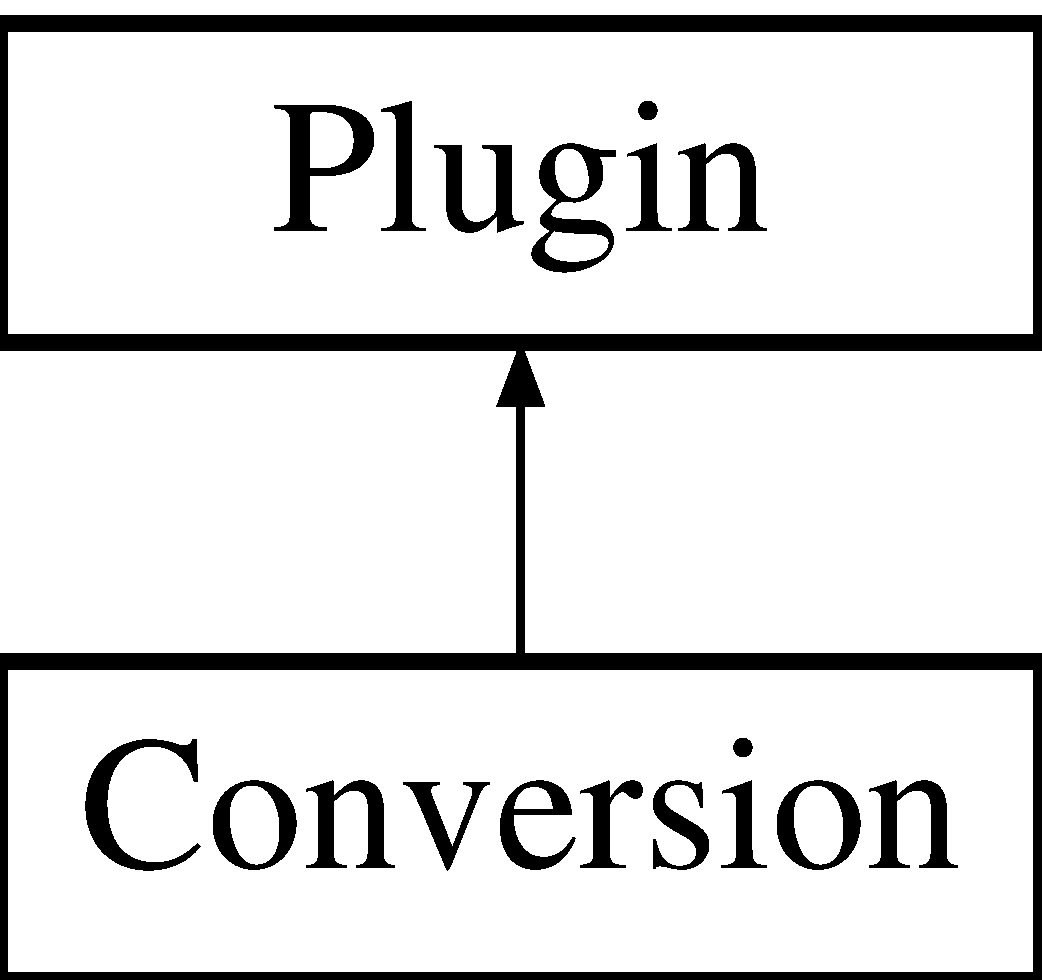
\includegraphics[height=2.000000cm]{dc/d41/classConversion}
\end{center}
\end{figure}
\subsection*{Public Member Functions}
\begin{DoxyCompactItemize}
\item 
\mbox{\Hypertarget{classConversion_a408cf455d1d4f2b1a1ba1a39d7996d11}\label{classConversion_a408cf455d1d4f2b1a1ba1a39d7996d11}} 
virtual \mbox{\hyperlink{classIndividual}{Individual}} $\ast$ {\bfseries convert} (const \mbox{\hyperlink{classIndividual}{Individual}} $\ast$ind, const int conf\+From, const int conf\+To)=0
\item 
\mbox{\Hypertarget{classConversion_a592abda114360f2a13af39c7de4be4cc}\label{classConversion_a592abda114360f2a13af39c7de4be4cc}} 
void {\bfseries set\+Alg\+Ind\+Pairs} (const vector$<$ pair$<$ string, string $>$ $>$ \&pairs)
\item 
\mbox{\Hypertarget{classConversion_ae8e8874a9af676204ec4f13a5f2643c9}\label{classConversion_ae8e8874a9af676204ec4f13a5f2643c9}} 
bool {\bfseries make\+Table\+Translation} (const vector$<$ pair$<$ string, string $>$ $>$ \&pairs\+Conv)
\item 
\mbox{\Hypertarget{classConversion_ac62754cf8a22c1c11591fe4260e0126e}\label{classConversion_ac62754cf8a22c1c11591fe4260e0126e}} 
bool {\bfseries make\+Table\+Translation} (const vector$<$ string $>$ \&alg)
\item 
\mbox{\Hypertarget{classConversion_aa05c692ce2bcad004aa465da169c6a34}\label{classConversion_aa05c692ce2bcad004aa465da169c6a34}} 
int {\bfseries get\+Translation} (int alg)
\item 
\mbox{\Hypertarget{classConversion_a2fdb1bb64d67a13d628d8c5a4ca1117c}\label{classConversion_a2fdb1bb64d67a13d628d8c5a4ca1117c}} 
void {\bfseries set\+Example\+Individuals} (vector$<$ \mbox{\hyperlink{classIndividual}{Individual}} $\ast$$>$ \&examples)
\end{DoxyCompactItemize}
\subsection*{Protected Attributes}
\begin{DoxyCompactItemize}
\item 
\mbox{\Hypertarget{classConversion_a2d748437e36c3487bd93f1242752ce50}\label{classConversion_a2d748437e36c3487bd93f1242752ce50}} 
vector$<$ \mbox{\hyperlink{classIndividual}{Individual}} $\ast$ $>$ {\bfseries example\+Individuals}
\item 
\mbox{\Hypertarget{classConversion_afc36a1c64fce3bf85a76bd81456298b1}\label{classConversion_afc36a1c64fce3bf85a76bd81456298b1}} 
vector$<$ pair$<$ string, string $>$ $>$ {\bfseries config\+File\+Pairs}
\item 
\mbox{\Hypertarget{classConversion_af1281db59d6b9de9d06c209221884104}\label{classConversion_af1281db59d6b9de9d06c209221884104}} 
vector$<$ int $>$ {\bfseries translation}
\end{DoxyCompactItemize}
\subsection*{Additional Inherited Members}


The documentation for this class was generated from the following files\+:\begin{DoxyCompactItemize}
\item 
Conversion.\+h\item 
Conversion.\+cpp\end{DoxyCompactItemize}

\hypertarget{classCoordinatorIsland}{}\section{Coordinator\+Island Class Reference}
\label{classCoordinatorIsland}\index{Coordinator\+Island@{Coordinator\+Island}}
\subsection*{Public Member Functions}
\begin{DoxyCompactItemize}
\item 
\mbox{\Hypertarget{classCoordinatorIsland_ab06731bdeed215595beebce0f087d967}\label{classCoordinatorIsland_ab06731bdeed215595beebce0f087d967}} 
{\bfseries Coordinator\+Island} (const string \&output\+File\+Name, const int print\+Period, const string \&base\+Directory)
\item 
\mbox{\Hypertarget{classCoordinatorIsland_aec9d72018c3681483e02da3b1aca90a9}\label{classCoordinatorIsland_aec9d72018c3681483e02da3b1aca90a9}} 
void {\bfseries run} (const char $\ast$file)
\item 
\mbox{\Hypertarget{classCoordinatorIsland_aa811da3292d8a8ee8c2b9041bea1cd2f}\label{classCoordinatorIsland_aa811da3292d8a8ee8c2b9041bea1cd2f}} 
\mbox{\hyperlink{classIndividual}{Individual}} $\ast$ {\bfseries get\+Ej\+Ind} () const
\item 
\mbox{\Hypertarget{classCoordinatorIsland_a1f2f4cbc23e2e571f25b2684a2cdc356}\label{classCoordinatorIsland_a1f2f4cbc23e2e571f25b2684a2cdc356}} 
int {\bfseries get\+Evaluations} () const
\item 
\mbox{\Hypertarget{classCoordinatorIsland_a979a3b6fc598652fb50479a069f3a08c}\label{classCoordinatorIsland_a979a3b6fc598652fb50479a069f3a08c}} 
ostream \& {\bfseries get\+Output\+File} ()
\item 
\mbox{\Hypertarget{classCoordinatorIsland_aaceb2bd1c34696257a6599d8671e126c}\label{classCoordinatorIsland_aaceb2bd1c34696257a6599d8671e126c}} 
const \mbox{\hyperlink{classConfiguration}{Configuration}} \& {\bfseries get\+Configuration} () const
\item 
\mbox{\Hypertarget{classCoordinatorIsland_a4a2824a1972075f41e2dcac9ea4bd6be}\label{classCoordinatorIsland_a4a2824a1972075f41e2dcac9ea4bd6be}} 
void {\bfseries get\+Solution} (\mbox{\hyperlink{classMOFront}{M\+O\+Front}} $\ast$p) const
\item 
\mbox{\Hypertarget{classCoordinatorIsland_a56f3dbd38c55b9363cad706228c588a2}\label{classCoordinatorIsland_a56f3dbd38c55b9363cad706228c588a2}} 
void {\bfseries print\+Info} (void)
\item 
\mbox{\Hypertarget{classCoordinatorIsland_afaadf2f86c49888e4194bbebdb96aa4d}\label{classCoordinatorIsland_afaadf2f86c49888e4194bbebdb96aa4d}} 
void {\bfseries print\+Characteristic} (const int num\+Slaves)
\item 
\mbox{\Hypertarget{classCoordinatorIsland_ad6f09de501f6ed21c6d7fce73937c4af}\label{classCoordinatorIsland_ad6f09de501f6ed21c6d7fce73937c4af}} 
void {\bfseries print\+Statistics} (void)
\end{DoxyCompactItemize}
\subsection*{Private Member Functions}
\begin{DoxyCompactItemize}
\item 
\mbox{\Hypertarget{classCoordinatorIsland_a8ef31c84fa543fc7a60e0e68b8f6d16e}\label{classCoordinatorIsland_a8ef31c84fa543fc7a60e0e68b8f6d16e}} 
void {\bfseries init} (const char $\ast$conf\+File)
\item 
\mbox{\Hypertarget{classCoordinatorIsland_af663b28b853073e2f5d179d19a28011f}\label{classCoordinatorIsland_af663b28b853073e2f5d179d19a28011f}} 
void {\bfseries init\+Islands} ()
\item 
\mbox{\Hypertarget{classCoordinatorIsland_a2637f5bc00df9693cf5b7bacdc9bc1fc}\label{classCoordinatorIsland_a2637f5bc00df9693cf5b7bacdc9bc1fc}} 
void {\bfseries init\+Algorithm} (const int act\+Alg, const int act\+Conf, const int id\+Island)
\item 
\mbox{\Hypertarget{classCoordinatorIsland_a78f74dd68e95864e0691e8a40b295e78}\label{classCoordinatorIsland_a78f74dd68e95864e0691e8a40b295e78}} 
void {\bfseries selection\+Island} (int \&index\+Alg, int \&config, const int idle)
\item 
\mbox{\Hypertarget{classCoordinatorIsland_a09cbbefa720138188302b340dd13bf69}\label{classCoordinatorIsland_a09cbbefa720138188302b340dd13bf69}} 
bool {\bfseries stop} ()
\item 
\mbox{\Hypertarget{classCoordinatorIsland_a9d6dfa8f43d2a2653eae788704b6e9e0}\label{classCoordinatorIsland_a9d6dfa8f43d2a2653eae788704b6e9e0}} 
bool {\bfseries stop\+Actual} ()
\item 
\mbox{\Hypertarget{classCoordinatorIsland_aec34100c82a854a961d39b881ef47145}\label{classCoordinatorIsland_aec34100c82a854a961d39b881ef47145}} 
void {\bfseries body\+Coordinator} (const int num\+Slaves)
\item 
\mbox{\Hypertarget{classCoordinatorIsland_a33f052e140a7c18109c35d58a12c82e4}\label{classCoordinatorIsland_a33f052e140a7c18109c35d58a12c82e4}} 
int {\bfseries recv\+Local\+Solution} ()
\item 
\mbox{\Hypertarget{classCoordinatorIsland_a5f05ee8573c776baa181e6e34fc31bec}\label{classCoordinatorIsland_a5f05ee8573c776baa181e6e34fc31bec}} 
void {\bfseries finish} (const int num\+Procs)
\item 
\mbox{\Hypertarget{classCoordinatorIsland_a52a6719766e8389a5f46ab6467df10bd}\label{classCoordinatorIsland_a52a6719766e8389a5f46ab6467df10bd}} 
long double {\bfseries score\+Configuration} (const int index\+Alg, const int config, const double rnd\+Value, const int island\+Id)
\item 
void \mbox{\hyperlink{classCoordinatorIsland_a25c1872d7c83a2e2855d2db4ada2f06d}{clear\+Statistics}} (vector$<$ vector$<$ \mbox{\hyperlink{structTStatistics}{T\+Statistics}} $>$ $>$ \&statistics)
\item 
\mbox{\Hypertarget{classCoordinatorIsland_a2e24a4b695b66ac53ea6176adeae64c0}\label{classCoordinatorIsland_a2e24a4b695b66ac53ea6176adeae64c0}} 
void {\bfseries check\+Print\+Period} ()
\end{DoxyCompactItemize}
\subsection*{Private Attributes}
\begin{DoxyCompactItemize}
\item 
\mbox{\Hypertarget{classCoordinatorIsland_a394481f37b842a1c374df49bc975b7de}\label{classCoordinatorIsland_a394481f37b842a1c374df49bc975b7de}} 
\mbox{\hyperlink{classConfiguration}{Configuration}} {\bfseries configuration}
\item 
\mbox{\Hypertarget{classCoordinatorIsland_af3303f59cee518348d9215d4c582084a}\label{classCoordinatorIsland_af3303f59cee518348d9215d4c582084a}} 
int {\bfseries num\+Procs}
\item 
\mbox{\Hypertarget{classCoordinatorIsland_a4f3ccbeaad01b52a00445697ba79ac65}\label{classCoordinatorIsland_a4f3ccbeaad01b52a00445697ba79ac65}} 
int {\bfseries not\+Used\+Islands}
\item 
\mbox{\Hypertarget{classCoordinatorIsland_ae982810359acf21091f829a27d5eba68}\label{classCoordinatorIsland_ae982810359acf21091f829a27d5eba68}} 
unsigned int {\bfseries actual\+Model}
\item 
\mbox{\Hypertarget{classCoordinatorIsland_ac7cbba9bde1ff274506bf78fcd7ca5f1}\label{classCoordinatorIsland_ac7cbba9bde1ff274506bf78fcd7ca5f1}} 
int {\bfseries my\+Id}
\item 
\mbox{\Hypertarget{classCoordinatorIsland_a1072839e49794db26dfc3170627b5b74}\label{classCoordinatorIsland_a1072839e49794db26dfc3170627b5b74}} 
\mbox{\hyperlink{classMOFront}{M\+O\+Front}} $\ast$ {\bfseries global\+Solution}
\item 
\mbox{\Hypertarget{classCoordinatorIsland_a319756886a25d4f53b383b4d36b3679f}\label{classCoordinatorIsland_a319756886a25d4f53b383b4d36b3679f}} 
double {\bfseries start\+Time}
\item 
\mbox{\Hypertarget{classCoordinatorIsland_ae777de209050b9f840d094051f29b7ad}\label{classCoordinatorIsland_ae777de209050b9f840d094051f29b7ad}} 
int {\bfseries num\+Executions}
\item 
\mbox{\Hypertarget{classCoordinatorIsland_a6a73b6222890a44a47c09b9279945f8e}\label{classCoordinatorIsland_a6a73b6222890a44a47c09b9279945f8e}} 
int {\bfseries print\+Period}
\item 
\mbox{\Hypertarget{classCoordinatorIsland_aedf88e408f4a17ee650807f03b42af71}\label{classCoordinatorIsland_aedf88e408f4a17ee650807f03b42af71}} 
int {\bfseries next\+Print}
\item 
\mbox{\Hypertarget{classCoordinatorIsland_a5d400b189383e2dd48d30c06a5db11d9}\label{classCoordinatorIsland_a5d400b189383e2dd48d30c06a5db11d9}} 
int {\bfseries evaluations}
\item 
\mbox{\Hypertarget{classCoordinatorIsland_a73c591a7ca9ee2723b95ba16b6b188ab}\label{classCoordinatorIsland_a73c591a7ca9ee2723b95ba16b6b188ab}} 
int {\bfseries evaluations\+Finished}
\item 
\mbox{\Hypertarget{classCoordinatorIsland_acef1ba13b24b23bc78cf4bdf37b8a06d}\label{classCoordinatorIsland_acef1ba13b24b23bc78cf4bdf37b8a06d}} 
double {\bfseries value\+Stop\+Crit}
\item 
\mbox{\Hypertarget{classCoordinatorIsland_a5af2468832745e66e19adc373c2f455c}\label{classCoordinatorIsland_a5af2468832745e66e19adc373c2f455c}} 
ofstream {\bfseries output\+File}
\item 
\mbox{\Hypertarget{classCoordinatorIsland_aaf187f409e882f32c88454974ac8e2b7}\label{classCoordinatorIsland_aaf187f409e882f32c88454974ac8e2b7}} 
string {\bfseries output\+File\+Name}
\item 
\mbox{\Hypertarget{classCoordinatorIsland_ab3aa5cc5aa936c6c508b4c1be6455cff}\label{classCoordinatorIsland_ab3aa5cc5aa936c6c508b4c1be6455cff}} 
queue$<$ int $>$ {\bfseries clear\+Statistic\+Evaluation}
\item 
\mbox{\Hypertarget{classCoordinatorIsland_ad7a9982659856df1c11922a5eb43c0a6}\label{classCoordinatorIsland_ad7a9982659856df1c11922a5eb43c0a6}} 
long double {\bfseries last\+Score}
\item 
\mbox{\Hypertarget{classCoordinatorIsland_abf6ec05de747be402ed0a4065a6ec336}\label{classCoordinatorIsland_abf6ec05de747be402ed0a4065a6ec336}} 
list$<$ \mbox{\hyperlink{structTTask}{T\+Task}} $>$ {\bfseries task\+Queue}
\item 
\mbox{\Hypertarget{classCoordinatorIsland_aeb5c8468d17ff38ef1c21f13c1940a75}\label{classCoordinatorIsland_aeb5c8468d17ff38ef1c21f13c1940a75}} 
list$<$ \mbox{\hyperlink{structTTask}{T\+Task}} $>$ {\bfseries circular\+Task\+Queue}
\item 
\mbox{\Hypertarget{classCoordinatorIsland_a5cb385deb46af49d24b6426af1c387c7}\label{classCoordinatorIsland_a5cb385deb46af49d24b6426af1c387c7}} 
vector$<$ vector$<$ \mbox{\hyperlink{structTStatistics}{T\+Statistics}} $>$ $>$ {\bfseries real\+Statistics}
\item 
\mbox{\Hypertarget{classCoordinatorIsland_a3b14bb913517f9c0041f948fca42245d}\label{classCoordinatorIsland_a3b14bb913517f9c0041f948fca42245d}} 
vector$<$ vector$<$ \mbox{\hyperlink{structTStatistics}{T\+Statistics}} $>$ $>$ {\bfseries used\+Statistics}
\item 
\mbox{\Hypertarget{classCoordinatorIsland_a4c4c0802869ba5e9c882a0463109d435}\label{classCoordinatorIsland_a4c4c0802869ba5e9c882a0463109d435}} 
vector$<$ int $>$ {\bfseries last\+Evaluations}
\item 
\mbox{\Hypertarget{classCoordinatorIsland_a592ffc45c62534e9dce75f600293a62c}\label{classCoordinatorIsland_a592ffc45c62534e9dce75f600293a62c}} 
vector$<$ int $>$ {\bfseries evaluations\+Performed}
\item 
\mbox{\Hypertarget{classCoordinatorIsland_ad0905830cccafc8991eddc85888560e4}\label{classCoordinatorIsland_ad0905830cccafc8991eddc85888560e4}} 
vector$<$ \mbox{\hyperlink{structTExecIsland}{T\+Exec\+Island}} $>$ {\bfseries exec\+Island}
\item 
\mbox{\Hypertarget{classCoordinatorIsland_ae7722d9300999fd9c97f58feb67f6a17}\label{classCoordinatorIsland_ae7722d9300999fd9c97f58feb67f6a17}} 
\mbox{\hyperlink{classInitPopIslandLoader}{Init\+Pop\+Island\+Loader}} $\ast$ {\bfseries ipil}
\item 
\mbox{\Hypertarget{classCoordinatorIsland_a12f619d43a6a4c160d0f3a6c38122cbe}\label{classCoordinatorIsland_a12f619d43a6a4c160d0f3a6c38122cbe}} 
int {\bfseries number\+Of\+Processes\+Per\+Execution}
\item 
\mbox{\Hypertarget{classCoordinatorIsland_ac3e7e32442c3ebbc99d6196a0bf0529c}\label{classCoordinatorIsland_ac3e7e32442c3ebbc99d6196a0bf0529c}} 
vector$<$ int $>$ {\bfseries my\+Slaves}
\end{DoxyCompactItemize}
\subsection*{Static Private Attributes}
\begin{DoxyCompactItemize}
\item 
\mbox{\Hypertarget{classCoordinatorIsland_a235933ff7bfb25907f929664f42d79ef}\label{classCoordinatorIsland_a235933ff7bfb25907f929664f42d79ef}} 
static const int {\bfseries P\+R\+I\+N\+T\+P\+E\+R\+I\+O\+D\+\_\+\+D\+E\+F\+A\+U\+LT} = 5000
\end{DoxyCompactItemize}


\subsection{Member Function Documentation}
\mbox{\Hypertarget{classCoordinatorIsland_a25c1872d7c83a2e2855d2db4ada2f06d}\label{classCoordinatorIsland_a25c1872d7c83a2e2855d2db4ada2f06d}} 
\index{Coordinator\+Island@{Coordinator\+Island}!clear\+Statistics@{clear\+Statistics}}
\index{clear\+Statistics@{clear\+Statistics}!Coordinator\+Island@{Coordinator\+Island}}
\subsubsection{\texorpdfstring{clear\+Statistics()}{clearStatistics()}}
{\footnotesize\ttfamily void Coordinator\+Island\+::clear\+Statistics (\begin{DoxyParamCaption}\item[{vector$<$ vector$<$ \mbox{\hyperlink{structTStatistics}{T\+Statistics}} $>$ $>$ \&}]{statistics }\end{DoxyParamCaption})\hspace{0.3cm}{\ttfamily [private]}}

!if (global\+Solution) 

The documentation for this class was generated from the following files\+:\begin{DoxyCompactItemize}
\item 
Coordinator\+Island.\+h\item 
Coordinator\+Island.\+cpp\end{DoxyCompactItemize}

\hypertarget{classCrossover}{}\section{Crossover Class Reference}
\label{classCrossover}\index{Crossover@{Crossover}}
Inheritance diagram for Crossover\+:\begin{figure}[H]
\begin{center}
\leavevmode
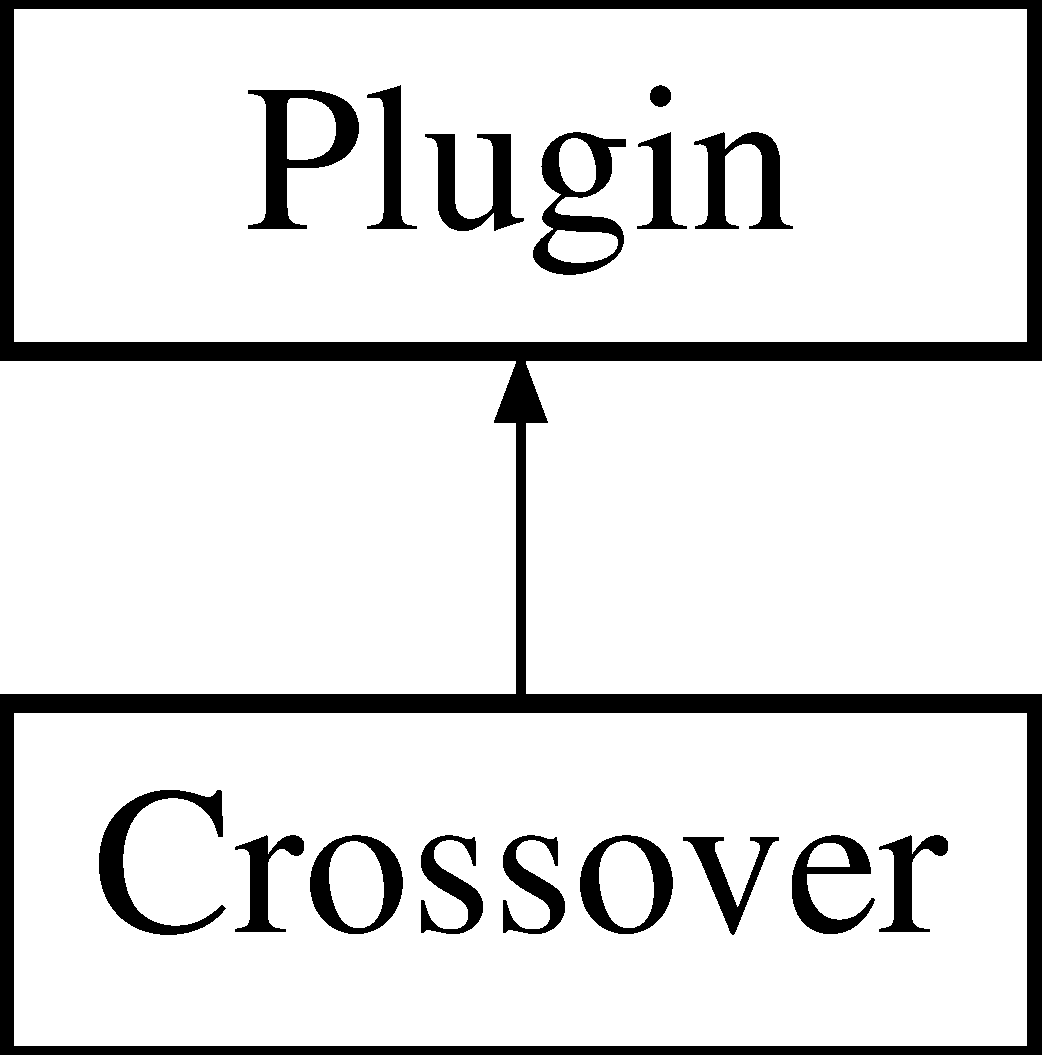
\includegraphics[height=2.000000cm]{da/dcc/classCrossover}
\end{center}
\end{figure}
\subsection*{Public Member Functions}
\begin{DoxyCompactItemize}
\item 
\mbox{\Hypertarget{classCrossover_ab116acf7d73233c76a6c906fc8d5edf6}\label{classCrossover_ab116acf7d73233c76a6c906fc8d5edf6}} 
virtual void {\bfseries crossover} (\mbox{\hyperlink{classIndividual}{Individual}} $\ast$ind1, \mbox{\hyperlink{classIndividual}{Individual}} $\ast$ind2)=0
\end{DoxyCompactItemize}
\subsection*{Additional Inherited Members}


The documentation for this class was generated from the following file\+:\begin{DoxyCompactItemize}
\item 
Crossover.\+h\end{DoxyCompactItemize}

\hypertarget{classEA}{}\section{EA Class Reference}
\label{classEA}\index{EA@{EA}}


\mbox{\hyperlink{classPlugin}{Plugin}} base class to represent the algorithms.  




{\ttfamily \#include $<$E\+A.\+h$>$}

Inheritance diagram for EA\+:\begin{figure}[H]
\begin{center}
\leavevmode
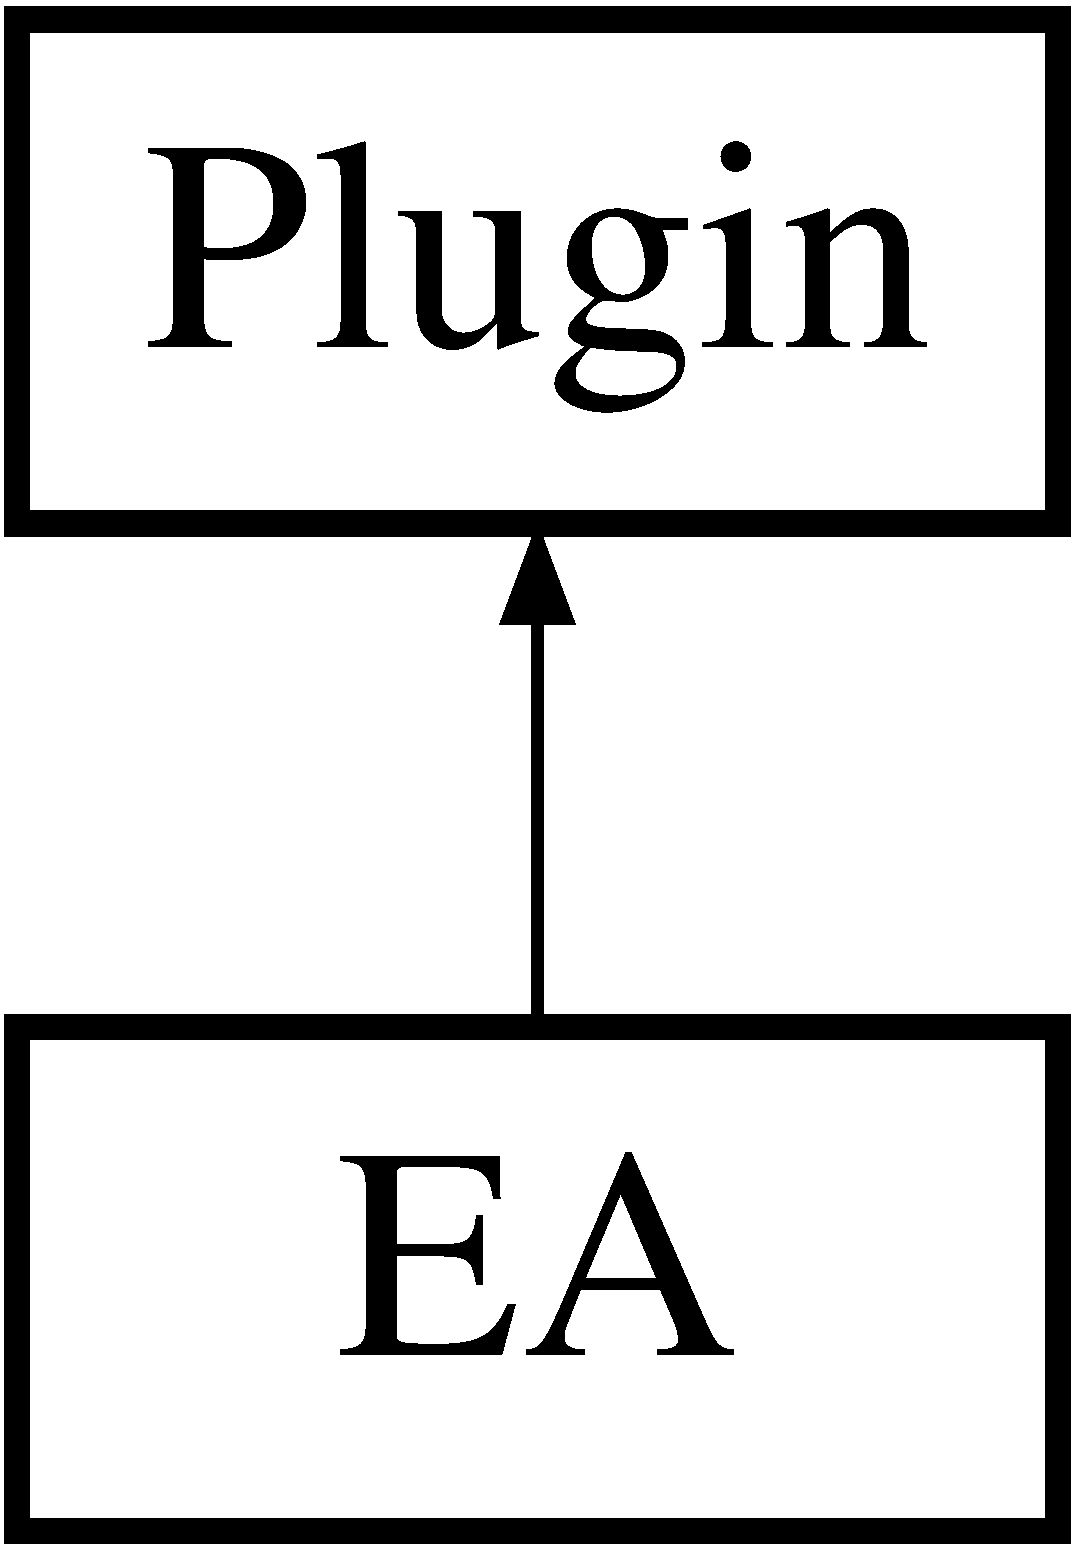
\includegraphics[height=2.000000cm]{d0/dff/classEA}
\end{center}
\end{figure}
\subsection*{Public Member Functions}
\begin{DoxyCompactItemize}
\item 
\mbox{\Hypertarget{classEA_aec8a2d9e63ecfc9705985e1994df0e67}\label{classEA_aec8a2d9e63ecfc9705985e1994df0e67}} 
\mbox{\hyperlink{classEA_aec8a2d9e63ecfc9705985e1994df0e67}{EA}} ()
\begin{DoxyCompactList}\small\item\em Constructor. \end{DoxyCompactList}\item 
\mbox{\Hypertarget{classEA_afad2dbe6e3835b1689ff2c62768eec30}\label{classEA_afad2dbe6e3835b1689ff2c62768eec30}} 
virtual \mbox{\hyperlink{classEA_afad2dbe6e3835b1689ff2c62768eec30}{$\sim$\+EA}} (void)
\begin{DoxyCompactList}\small\item\em Destructor. \end{DoxyCompactList}\item 
virtual void \mbox{\hyperlink{classEA_a84eacf2682007bef9f90543ecdd0639e}{get\+Solution}} (\mbox{\hyperlink{classMOFront}{M\+O\+Front}} $\ast$p)=0
\begin{DoxyCompactList}\small\item\em This methods must copy all the solution into the Pareto\textquotesingle{}s Front. \end{DoxyCompactList}\item 
virtual void \mbox{\hyperlink{classEA_a2c495b6198538ee0ecbef9d18ced1f61}{print\+Info}} (ostream \&os) const =0
\begin{DoxyCompactList}\small\item\em This method must be overwritten in order to print the information of the algorithm. \end{DoxyCompactList}\item 
\mbox{\Hypertarget{classEA_a88b3f36c7e82d4f19d5b5b6720c42416}\label{classEA_a88b3f36c7e82d4f19d5b5b6720c42416}} 
virtual void {\bfseries received} (vector$<$ \mbox{\hyperlink{classIndividual}{Individual}} $\ast$$>$ \&)
\item 
\mbox{\Hypertarget{classEA_aa7ce22145328a30ed9f53009f33e80c4}\label{classEA_aa7ce22145328a30ed9f53009f33e80c4}} 
virtual double $\ast$ {\bfseries get\+Restart\+Info} ()
\item 
\mbox{\Hypertarget{classEA_aa628b1461589a9d6773be9d10ef1636c}\label{classEA_aa628b1461589a9d6773be9d10ef1636c}} 
virtual void {\bfseries set\+Restart\+Info} (double $\ast$)
\item 
\mbox{\Hypertarget{classEA_a2b293ab31ea89d16e14f313332f76074}\label{classEA_a2b293ab31ea89d16e14f313332f76074}} 
virtual void {\bfseries exchange\+Performed} ()
\item 
\mbox{\Hypertarget{classEA_a0b330cfc98d799706ebaee44dfbfdd21}\label{classEA_a0b330cfc98d799706ebaee44dfbfdd21}} 
void \mbox{\hyperlink{classEA_a0b330cfc98d799706ebaee44dfbfdd21}{run}} ()
\begin{DoxyCompactList}\small\item\em Run the algorithm. \end{DoxyCompactList}\item 
void \mbox{\hyperlink{classEA_a6ab8cb75b4a102d91579a58ecb815f6c}{fill\+Pop\+With\+Evaluated\+Inds}} (const vector$<$ \mbox{\hyperlink{classIndividual}{Individual}} $\ast$$>$ \&)
\begin{DoxyCompactList}\small\item\em Initialize the initial population with individuals from Global Front. \end{DoxyCompactList}\item 
\mbox{\Hypertarget{classEA_a8a4518d405abf91c5432b8823d34c400}\label{classEA_a8a4518d405abf91c5432b8823d34c400}} 
void \mbox{\hyperlink{classEA_a8a4518d405abf91c5432b8823d34c400}{run\+Generation\+Inc}} ()
\begin{DoxyCompactList}\small\item\em Increments the generation counter. \end{DoxyCompactList}\item 
bool \mbox{\hyperlink{classEA_a1ef25307a0576f54ea6009d4c94c9d48}{has\+Finished}} ()
\begin{DoxyCompactList}\small\item\em Checks if the algorithm has finished yet. \end{DoxyCompactList}\item 
void \mbox{\hyperlink{classEA_ad56460c346eca5b890b27c85e985ec12}{reset\+Stop\+Conditions}} ()
\begin{DoxyCompactList}\small\item\em Restars the stopping condition. \end{DoxyCompactList}\item 
void \mbox{\hyperlink{classEA_a65e719d5e3a3cff67139d1e81f092cec}{evaluate}} (\mbox{\hyperlink{classIndividual}{Individual}} $\ast$ind)
\begin{DoxyCompactList}\small\item\em Evaluate the given individual with its evaluation function This methods must call the evaluate method from \mbox{\hyperlink{classIndividual}{Individual}} class. \end{DoxyCompactList}\item 
\mbox{\Hypertarget{classEA_a208ac74dea2eaa42e17c19f5e32d644d}\label{classEA_a208ac74dea2eaa42e17c19f5e32d644d}} 
void {\bfseries insert\+In\+Archive} (\mbox{\hyperlink{classIndividual}{Individual}} $\ast$ind)
\item 
void \mbox{\hyperlink{classEA_afb4678f700cb03d64dc60fc3d24f7a1f}{set\+Population\+Size}} (const int p\+Size)
\begin{DoxyCompactList}\small\item\em Set the population size. \end{DoxyCompactList}\item 
void \mbox{\hyperlink{classEA_add9a924cd307b2a49b1cf961c65e8ef2}{set\+Sample\+Ind}} (\mbox{\hyperlink{classIndividual}{Individual}} $\ast$ind)
\begin{DoxyCompactList}\small\item\em Set a sample \mbox{\hyperlink{classIndividual}{Individual}}. \end{DoxyCompactList}\item 
void \mbox{\hyperlink{classEA_a49a75271ab62ffdb59d7a5fbbc97f998}{set\+Output\+Printer}} (\mbox{\hyperlink{classOutputPrinter}{Output\+Printer}} $\ast$op)
\begin{DoxyCompactList}\small\item\em Set printer module from \mbox{\hyperlink{classOutputPrinter}{Output\+Printer}} instances. \end{DoxyCompactList}\item 
void \mbox{\hyperlink{classEA_a161b549d8ec90da1bd07687f6b388b59}{set\+Print\+Period}} (const int pp)
\begin{DoxyCompactList}\small\item\em Set the period to print the intermediate results. \end{DoxyCompactList}\item 
void \mbox{\hyperlink{classEA_a114980c167652af030f11349810797e9}{set\+Max\+Local\+Front\+Size}} (const int max)
\begin{DoxyCompactList}\small\item\em Set the maximum number of individuals in the Pareto\textquotesingle{}s Front. \end{DoxyCompactList}\item 
\mbox{\Hypertarget{classEA_a2140dd732a9acc2ce6044669e60bb335}\label{classEA_a2140dd732a9acc2ce6044669e60bb335}} 
void {\bfseries set\+Score\+Algorithm} (\mbox{\hyperlink{classScoreAlgorithm}{Score\+Algorithm}} $\ast$sc)
\item 
\mbox{\Hypertarget{classEA_a7331ed1b01abe48b170068abbde388be}\label{classEA_a7331ed1b01abe48b170068abbde388be}} 
void {\bfseries set\+Local\+Search} (\mbox{\hyperlink{classLocalSearch}{Local\+Search}} $\ast$ls)
\item 
\mbox{\Hypertarget{classEA_a73cb790a9ba0a552096613522c13d6cf}\label{classEA_a73cb790a9ba0a552096613522c13d6cf}} 
void {\bfseries set\+Multi\+Objectivization\+Plugins} (const vector$<$ \mbox{\hyperlink{classMultiObjectivization}{Multi\+Objectivization}} $\ast$$>$ \&multi)
\item 
\mbox{\Hypertarget{classEA_a4e6f4130156dc99c0c44f9d7b9903a25}\label{classEA_a4e6f4130156dc99c0c44f9d7b9903a25}} 
void {\bfseries set\+Generate\+Archive} (const bool generate, const int type)
\item 
void \mbox{\hyperlink{classEA_a61c0385f3596233e124a9002e834fc6a}{set\+Stopping\+Criterion}} (const int crit\+Stop, const double crit\+Stop\+Value)
\begin{DoxyCompactList}\small\item\em Initialize the necessary attributes to set a stopping criteria. \end{DoxyCompactList}\item 
int \mbox{\hyperlink{classEA_a6ec89c4b5edec15a2c59f8f640522169}{get\+Crit\+Stop}} (void) const
\begin{DoxyCompactList}\small\item\em Method that returns the stopping criteria. \end{DoxyCompactList}\item 
double \mbox{\hyperlink{classEA_a53c6bb76e024220eae10799b732d1571}{get\+Crit\+Stop\+Value}} (void) const
\begin{DoxyCompactList}\small\item\em This method returns the value for the stopping criteria. \end{DoxyCompactList}\item 
int \mbox{\hyperlink{classEA_af3137eadac064eb1257ec161150fb304}{get\+Print\+Period}} (void) const
\begin{DoxyCompactList}\small\item\em Returns how many iterations the algorithm must print the results. \end{DoxyCompactList}\item 
int \mbox{\hyperlink{classEA_a107a7507708a8a4db8ca2dfbef72f52c}{get\+Population\+Size}} (void) const
\begin{DoxyCompactList}\small\item\em This method returns how many individuals are in the population. \end{DoxyCompactList}\item 
\mbox{\Hypertarget{classEA_a0bb927fe460bab1aa745ac9df0b267c9}\label{classEA_a0bb927fe460bab1aa745ac9df0b267c9}} 
\mbox{\hyperlink{classMOFront}{M\+O\+Front}} $\ast$ {\bfseries get\+Local\+Solution} (void) const
\item 
int \mbox{\hyperlink{classEA_ad677d015c33f989e079eb9b204f1dd3c}{get\+Evaluations}} (void) const
\begin{DoxyCompactList}\small\item\em Method that returns the number of maximum evaluations to perform. \end{DoxyCompactList}\item 
int \mbox{\hyperlink{classEA_ab40a86dcc65d506f7327e457e137859f}{get\+Performed\+Evaluations}} (void) const
\begin{DoxyCompactList}\small\item\em Method that returns the number of performed evaluations. \end{DoxyCompactList}\item 
int \mbox{\hyperlink{classEA_a6fd5e97e8a83ed5b187311cc77c246f5}{get\+Generation}} (void) const
\begin{DoxyCompactList}\small\item\em Method that returns the number of generations. \end{DoxyCompactList}\item 
int \mbox{\hyperlink{classEA_ae84da938d98677fa658c2b3659a7c356}{get\+Max\+Local\+Front\+Size}} (void) const
\begin{DoxyCompactList}\small\item\em Method that returns the number of maximum individuals in the Pareto\textquotesingle{}s Front. \end{DoxyCompactList}\item 
\mbox{\Hypertarget{classEA_aced3f2cb4a4825b1a2df6e7b220433f8}\label{classEA_aced3f2cb4a4825b1a2df6e7b220433f8}} 
\mbox{\hyperlink{classIndividual}{Individual}} $\ast$ {\bfseries get\+Sample\+Ind} (void) const
\item 
\mbox{\Hypertarget{classEA_a4e9f31e6d33381156b6c86805172568f}\label{classEA_a4e9f31e6d33381156b6c86805172568f}} 
bool {\bfseries is\+Generating\+Archive} (void) const
\item 
\mbox{\Hypertarget{classEA_aed2699ea33f0fcfb93a5dda4008642a3}\label{classEA_aed2699ea33f0fcfb93a5dda4008642a3}} 
int {\bfseries get\+Next\+Print} (void) const
\item 
\mbox{\Hypertarget{classEA_aefd916d9b6c470c24572f78e4e7a7c63}\label{classEA_aefd916d9b6c470c24572f78e4e7a7c63}} 
\mbox{\hyperlink{classMultiObjectivization}{Multi\+Objectivization}} $\ast$ {\bfseries get\+Multi\+Objectivization\+Plugin} (int index) const
\item 
\mbox{\Hypertarget{classEA_a7893ceefbafe8ecef3107626bfd55ef3}\label{classEA_a7893ceefbafe8ecef3107626bfd55ef3}} 
int {\bfseries get\+Num\+Multi\+Objectivization\+Plugins} (void) const
\item 
double \mbox{\hyperlink{classEA_ad2ab19a63b1222c13f67009ac2df972d}{get\+Elapsed\+Time}} () const
\begin{DoxyCompactList}\small\item\em This method returns the elapsed time of the execution. \end{DoxyCompactList}\item 
\mbox{\Hypertarget{classEA_a610f12a2674c608c3bc4cac93e243ebf}\label{classEA_a610f12a2674c608c3bc4cac93e243ebf}} 
virtual bool {\bfseries supports\+Multi\+Objectivization} ()
\end{DoxyCompactItemize}
\subsection*{Static Public Member Functions}
\begin{DoxyCompactItemize}
\item 
\mbox{\Hypertarget{classEA_a487729de3d170cab56f0617604aeac90}\label{classEA_a487729de3d170cab56f0617604aeac90}} 
static string {\bfseries get\+Global\+Type\+Stop\+Crit} (const int i)
\item 
\mbox{\Hypertarget{classEA_a67a3533562f15f67589ae6cbfaf07aa8}\label{classEA_a67a3533562f15f67589ae6cbfaf07aa8}} 
static int {\bfseries get\+Type\+Stopping\+Criterion} (const string \&cr)
\end{DoxyCompactItemize}
\subsection*{Protected Member Functions}
\begin{DoxyCompactItemize}
\item 
\mbox{\Hypertarget{classEA_a9dc2d07361618fa82c9a70e125fc490d}\label{classEA_a9dc2d07361618fa82c9a70e125fc490d}} 
int {\bfseries binary\+Tournament} (vector$<$ \mbox{\hyperlink{classIndividual}{Individual}} $\ast$$>$ $\ast$pop)
\end{DoxyCompactItemize}
\subsection*{Protected Attributes}
\begin{DoxyCompactItemize}
\item 
\mbox{\Hypertarget{classEA_abb8743d21c3db992b53356e1d8fe2646}\label{classEA_abb8743d21c3db992b53356e1d8fe2646}} 
vector$<$ \mbox{\hyperlink{classIndividual}{Individual}} $\ast$ $>$ $\ast$ \mbox{\hyperlink{classEA_abb8743d21c3db992b53356e1d8fe2646}{population}}
\begin{DoxyCompactList}\small\item\em Vector of \mbox{\hyperlink{classIndividual}{Individual}} instances that shape the population. \end{DoxyCompactList}\end{DoxyCompactItemize}
\subsection*{Private Member Functions}
\begin{DoxyCompactItemize}
\item 
virtual void \mbox{\hyperlink{classEA_ab5586c481933e063694c45d487757c82}{run\+Generation}} ()=0
\begin{DoxyCompactList}\small\item\em Method that run one generation of the algorithm. \end{DoxyCompactList}\item 
virtual void \mbox{\hyperlink{classEA_ae99a3c887d3014a59bce9501add80308}{fill\+Pop\+With\+New\+Inds\+And\+Evaluate}} ()
\begin{DoxyCompactList}\small\item\em Method fill the population with new individuals and then, evaluate them. \end{DoxyCompactList}\end{DoxyCompactItemize}
\subsection*{Private Attributes}
\begin{DoxyCompactItemize}
\item 
\mbox{\hyperlink{classIndividual}{Individual}} $\ast$ \mbox{\hyperlink{classEA_aee2992080a3ffc95c9edea9cc142f62d}{sample\+Ind}}
\begin{DoxyCompactList}\small\item\em Sample \mbox{\hyperlink{classIndividual}{Individual}}. \end{DoxyCompactList}\item 
\mbox{\Hypertarget{classEA_a003551d80fd0fd6e7bc29870ec1b2bd8}\label{classEA_a003551d80fd0fd6e7bc29870ec1b2bd8}} 
\mbox{\hyperlink{classOutputPrinter}{Output\+Printer}} $\ast$ \mbox{\hyperlink{classEA_a003551d80fd0fd6e7bc29870ec1b2bd8}{output\+Printer}}
\begin{DoxyCompactList}\small\item\em \mbox{\hyperlink{classOutputPrinter}{Output\+Printer}} instance to print the results. \end{DoxyCompactList}\item 
\mbox{\Hypertarget{classEA_a340f68daee20bce5089deed405edb791}\label{classEA_a340f68daee20bce5089deed405edb791}} 
\mbox{\hyperlink{classMOFront}{M\+O\+Front}} $\ast$ {\bfseries local\+Solution}
\item 
\mbox{\Hypertarget{classEA_ad4c30ccbc633bfa530fa50ca0970bd18}\label{classEA_ad4c30ccbc633bfa530fa50ca0970bd18}} 
\mbox{\hyperlink{classLocalScoreAlgorithm}{Local\+Score\+Algorithm}} $\ast$ {\bfseries score\+Algorithm}
\item 
\mbox{\Hypertarget{classEA_aeba2a26cf290afd924fbafbd0c4ad64d}\label{classEA_aeba2a26cf290afd924fbafbd0c4ad64d}} 
\mbox{\hyperlink{classLocalSearch}{Local\+Search}} $\ast$ {\bfseries ls}
\item 
\mbox{\Hypertarget{classEA_a3acbcb04351627ec86125084c251e12d}\label{classEA_a3acbcb04351627ec86125084c251e12d}} 
int {\bfseries crit\+Stop}
\item 
\mbox{\Hypertarget{classEA_ad7cefa1c91b348cf8436f49ae83560d6}\label{classEA_ad7cefa1c91b348cf8436f49ae83560d6}} 
int {\bfseries evaluations}
\item 
\mbox{\Hypertarget{classEA_ad612447f4ae22f8c1b651c7d18471846}\label{classEA_ad612447f4ae22f8c1b651c7d18471846}} 
int {\bfseries evaluation\+Actual}
\item 
\mbox{\Hypertarget{classEA_ac5a4cf8f9e12dfc07f8d4d4019e89540}\label{classEA_ac5a4cf8f9e12dfc07f8d4d4019e89540}} 
int {\bfseries generations}
\item 
\mbox{\Hypertarget{classEA_a7c2e3fae5ef87767765d58d9637e0d29}\label{classEA_a7c2e3fae5ef87767765d58d9637e0d29}} 
int {\bfseries generation\+Actual}
\item 
double \mbox{\hyperlink{classEA_ad62e844dcae9b5c7724ab56a9aea2dc9}{quality}}
\begin{DoxyCompactList}\small\item\em Desired quality to finish the execution. \end{DoxyCompactList}\item 
\mbox{\Hypertarget{classEA_add005610c438f386a0e1297f40f99294}\label{classEA_add005610c438f386a0e1297f40f99294}} 
int {\bfseries local\+Front\+Size}
\item 
\mbox{\Hypertarget{classEA_a76be177471c03a1c37b2e562d0ad51cf}\label{classEA_a76be177471c03a1c37b2e562d0ad51cf}} 
double {\bfseries time}
\item 
\mbox{\Hypertarget{classEA_af18fabb320c08ef9de16fd9877272211}\label{classEA_af18fabb320c08ef9de16fd9877272211}} 
double {\bfseries crit\+Stop\+Value}
\item 
\mbox{\Hypertarget{classEA_a40edcfb8016401e5ea73b8188731026b}\label{classEA_a40edcfb8016401e5ea73b8188731026b}} 
vector$<$ \mbox{\hyperlink{classMultiObjectivization}{Multi\+Objectivization}} $\ast$ $>$ {\bfseries multi\+Objectivizations\+Plugins}
\end{DoxyCompactItemize}
\subsection*{Additional Inherited Members}


\subsection{Detailed Description}
\mbox{\hyperlink{classPlugin}{Plugin}} base class to represent the algorithms. 

\subsection{Member Function Documentation}
\mbox{\Hypertarget{classEA_a65e719d5e3a3cff67139d1e81f092cec}\label{classEA_a65e719d5e3a3cff67139d1e81f092cec}} 
\index{EA@{EA}!evaluate@{evaluate}}
\index{evaluate@{evaluate}!EA@{EA}}
\subsubsection{\texorpdfstring{evaluate()}{evaluate()}}
{\footnotesize\ttfamily void E\+A\+::evaluate (\begin{DoxyParamCaption}\item[{\mbox{\hyperlink{classIndividual}{Individual}} $\ast$}]{ind }\end{DoxyParamCaption})}



Evaluate the given individual with its evaluation function This methods must call the evaluate method from \mbox{\hyperlink{classIndividual}{Individual}} class. 


\begin{DoxyParams}{Parameters}
{\em \mbox{\hyperlink{classIndividual}{Individual}}} & to be evaluated \\
\hline
\end{DoxyParams}
\mbox{\Hypertarget{classEA_a6ab8cb75b4a102d91579a58ecb815f6c}\label{classEA_a6ab8cb75b4a102d91579a58ecb815f6c}} 
\index{EA@{EA}!fill\+Pop\+With\+Evaluated\+Inds@{fill\+Pop\+With\+Evaluated\+Inds}}
\index{fill\+Pop\+With\+Evaluated\+Inds@{fill\+Pop\+With\+Evaluated\+Inds}!EA@{EA}}
\subsubsection{\texorpdfstring{fill\+Pop\+With\+Evaluated\+Inds()}{fillPopWithEvaluatedInds()}}
{\footnotesize\ttfamily void E\+A\+::fill\+Pop\+With\+Evaluated\+Inds (\begin{DoxyParamCaption}\item[{const vector$<$ \mbox{\hyperlink{classIndividual}{Individual}} $\ast$$>$ \&}]{new\+Inds }\end{DoxyParamCaption})}



Initialize the initial population with individuals from Global Front. 


\begin{DoxyParams}{Parameters}
{\em Vector$<$\+Individual} & $\ast$$>$ Evaluated individuals \\
\hline
\end{DoxyParams}
\mbox{\Hypertarget{classEA_ae99a3c887d3014a59bce9501add80308}\label{classEA_ae99a3c887d3014a59bce9501add80308}} 
\index{EA@{EA}!fill\+Pop\+With\+New\+Inds\+And\+Evaluate@{fill\+Pop\+With\+New\+Inds\+And\+Evaluate}}
\index{fill\+Pop\+With\+New\+Inds\+And\+Evaluate@{fill\+Pop\+With\+New\+Inds\+And\+Evaluate}!EA@{EA}}
\subsubsection{\texorpdfstring{fill\+Pop\+With\+New\+Inds\+And\+Evaluate()}{fillPopWithNewIndsAndEvaluate()}}
{\footnotesize\ttfamily void E\+A\+::fill\+Pop\+With\+New\+Inds\+And\+Evaluate (\begin{DoxyParamCaption}{ }\end{DoxyParamCaption})\hspace{0.3cm}{\ttfamily [private]}, {\ttfamily [virtual]}}



Method fill the population with new individuals and then, evaluate them. 

This method could be overwritten by the sub-\/classes. \mbox{\Hypertarget{classEA_a6ec89c4b5edec15a2c59f8f640522169}\label{classEA_a6ec89c4b5edec15a2c59f8f640522169}} 
\index{EA@{EA}!get\+Crit\+Stop@{get\+Crit\+Stop}}
\index{get\+Crit\+Stop@{get\+Crit\+Stop}!EA@{EA}}
\subsubsection{\texorpdfstring{get\+Crit\+Stop()}{getCritStop()}}
{\footnotesize\ttfamily int E\+A\+::get\+Crit\+Stop (\begin{DoxyParamCaption}\item[{void}]{ }\end{DoxyParamCaption}) const\hspace{0.3cm}{\ttfamily [inline]}}



Method that returns the stopping criteria. 

\begin{DoxyReturn}{Returns}
The actual stopping criteria 
\end{DoxyReturn}
\mbox{\Hypertarget{classEA_a53c6bb76e024220eae10799b732d1571}\label{classEA_a53c6bb76e024220eae10799b732d1571}} 
\index{EA@{EA}!get\+Crit\+Stop\+Value@{get\+Crit\+Stop\+Value}}
\index{get\+Crit\+Stop\+Value@{get\+Crit\+Stop\+Value}!EA@{EA}}
\subsubsection{\texorpdfstring{get\+Crit\+Stop\+Value()}{getCritStopValue()}}
{\footnotesize\ttfamily double E\+A\+::get\+Crit\+Stop\+Value (\begin{DoxyParamCaption}\item[{void}]{ }\end{DoxyParamCaption}) const\hspace{0.3cm}{\ttfamily [inline]}}



This method returns the value for the stopping criteria. 

\begin{DoxyReturn}{Returns}
The stopping criteria value 
\end{DoxyReturn}
\mbox{\Hypertarget{classEA_ad2ab19a63b1222c13f67009ac2df972d}\label{classEA_ad2ab19a63b1222c13f67009ac2df972d}} 
\index{EA@{EA}!get\+Elapsed\+Time@{get\+Elapsed\+Time}}
\index{get\+Elapsed\+Time@{get\+Elapsed\+Time}!EA@{EA}}
\subsubsection{\texorpdfstring{get\+Elapsed\+Time()}{getElapsedTime()}}
{\footnotesize\ttfamily double E\+A\+::get\+Elapsed\+Time (\begin{DoxyParamCaption}{ }\end{DoxyParamCaption}) const}



This method returns the elapsed time of the execution. 

\begin{DoxyReturn}{Returns}
Elapsed time 
\end{DoxyReturn}
\mbox{\Hypertarget{classEA_ad677d015c33f989e079eb9b204f1dd3c}\label{classEA_ad677d015c33f989e079eb9b204f1dd3c}} 
\index{EA@{EA}!get\+Evaluations@{get\+Evaluations}}
\index{get\+Evaluations@{get\+Evaluations}!EA@{EA}}
\subsubsection{\texorpdfstring{get\+Evaluations()}{getEvaluations()}}
{\footnotesize\ttfamily int E\+A\+::get\+Evaluations (\begin{DoxyParamCaption}\item[{void}]{ }\end{DoxyParamCaption}) const\hspace{0.3cm}{\ttfamily [inline]}}



Method that returns the number of maximum evaluations to perform. 

\begin{DoxyReturn}{Returns}
Maximum evaluations to perform 
\end{DoxyReturn}
\mbox{\Hypertarget{classEA_a6fd5e97e8a83ed5b187311cc77c246f5}\label{classEA_a6fd5e97e8a83ed5b187311cc77c246f5}} 
\index{EA@{EA}!get\+Generation@{get\+Generation}}
\index{get\+Generation@{get\+Generation}!EA@{EA}}
\subsubsection{\texorpdfstring{get\+Generation()}{getGeneration()}}
{\footnotesize\ttfamily int E\+A\+::get\+Generation (\begin{DoxyParamCaption}\item[{void}]{ }\end{DoxyParamCaption}) const\hspace{0.3cm}{\ttfamily [inline]}}



Method that returns the number of generations. 

\begin{DoxyReturn}{Returns}
Current generation. 
\end{DoxyReturn}
\mbox{\Hypertarget{classEA_ae84da938d98677fa658c2b3659a7c356}\label{classEA_ae84da938d98677fa658c2b3659a7c356}} 
\index{EA@{EA}!get\+Max\+Local\+Front\+Size@{get\+Max\+Local\+Front\+Size}}
\index{get\+Max\+Local\+Front\+Size@{get\+Max\+Local\+Front\+Size}!EA@{EA}}
\subsubsection{\texorpdfstring{get\+Max\+Local\+Front\+Size()}{getMaxLocalFrontSize()}}
{\footnotesize\ttfamily int E\+A\+::get\+Max\+Local\+Front\+Size (\begin{DoxyParamCaption}\item[{void}]{ }\end{DoxyParamCaption}) const\hspace{0.3cm}{\ttfamily [inline]}}



Method that returns the number of maximum individuals in the Pareto\textquotesingle{}s Front. 

\begin{DoxyReturn}{Returns}
Maximum number of individuals in the Pareto\textquotesingle{}s Front 
\end{DoxyReturn}
\mbox{\Hypertarget{classEA_ab40a86dcc65d506f7327e457e137859f}\label{classEA_ab40a86dcc65d506f7327e457e137859f}} 
\index{EA@{EA}!get\+Performed\+Evaluations@{get\+Performed\+Evaluations}}
\index{get\+Performed\+Evaluations@{get\+Performed\+Evaluations}!EA@{EA}}
\subsubsection{\texorpdfstring{get\+Performed\+Evaluations()}{getPerformedEvaluations()}}
{\footnotesize\ttfamily int E\+A\+::get\+Performed\+Evaluations (\begin{DoxyParamCaption}\item[{void}]{ }\end{DoxyParamCaption}) const\hspace{0.3cm}{\ttfamily [inline]}}



Method that returns the number of performed evaluations. 

\begin{DoxyReturn}{Returns}
Performed evaluations 
\end{DoxyReturn}
\mbox{\Hypertarget{classEA_a107a7507708a8a4db8ca2dfbef72f52c}\label{classEA_a107a7507708a8a4db8ca2dfbef72f52c}} 
\index{EA@{EA}!get\+Population\+Size@{get\+Population\+Size}}
\index{get\+Population\+Size@{get\+Population\+Size}!EA@{EA}}
\subsubsection{\texorpdfstring{get\+Population\+Size()}{getPopulationSize()}}
{\footnotesize\ttfamily int E\+A\+::get\+Population\+Size (\begin{DoxyParamCaption}\item[{void}]{ }\end{DoxyParamCaption}) const\hspace{0.3cm}{\ttfamily [inline]}}



This method returns how many individuals are in the population. 

\begin{DoxyReturn}{Returns}
Population size 
\end{DoxyReturn}
\mbox{\Hypertarget{classEA_af3137eadac064eb1257ec161150fb304}\label{classEA_af3137eadac064eb1257ec161150fb304}} 
\index{EA@{EA}!get\+Print\+Period@{get\+Print\+Period}}
\index{get\+Print\+Period@{get\+Print\+Period}!EA@{EA}}
\subsubsection{\texorpdfstring{get\+Print\+Period()}{getPrintPeriod()}}
{\footnotesize\ttfamily int E\+A\+::get\+Print\+Period (\begin{DoxyParamCaption}\item[{void}]{ }\end{DoxyParamCaption}) const\hspace{0.3cm}{\ttfamily [inline]}}



Returns how many iterations the algorithm must print the results. 

\begin{DoxyReturn}{Returns}
Number of iterations to print the results 
\end{DoxyReturn}
\mbox{\Hypertarget{classEA_a84eacf2682007bef9f90543ecdd0639e}\label{classEA_a84eacf2682007bef9f90543ecdd0639e}} 
\index{EA@{EA}!get\+Solution@{get\+Solution}}
\index{get\+Solution@{get\+Solution}!EA@{EA}}
\subsubsection{\texorpdfstring{get\+Solution()}{getSolution()}}
{\footnotesize\ttfamily virtual void E\+A\+::get\+Solution (\begin{DoxyParamCaption}\item[{\mbox{\hyperlink{classMOFront}{M\+O\+Front}} $\ast$}]{p }\end{DoxyParamCaption})\hspace{0.3cm}{\ttfamily [pure virtual]}}



This methods must copy all the solution into the Pareto\textquotesingle{}s Front. 


\begin{DoxyParams}{Parameters}
{\em } & M\+O\+Front$\ast$ Empty Pareto\textquotesingle{}s Front \\
\hline
\end{DoxyParams}
\mbox{\Hypertarget{classEA_a1ef25307a0576f54ea6009d4c94c9d48}\label{classEA_a1ef25307a0576f54ea6009d4c94c9d48}} 
\index{EA@{EA}!has\+Finished@{has\+Finished}}
\index{has\+Finished@{has\+Finished}!EA@{EA}}
\subsubsection{\texorpdfstring{has\+Finished()}{hasFinished()}}
{\footnotesize\ttfamily bool E\+A\+::has\+Finished (\begin{DoxyParamCaption}{ }\end{DoxyParamCaption})}



Checks if the algorithm has finished yet. 

The stopping criteria has been reached. \mbox{\Hypertarget{classEA_a2c495b6198538ee0ecbef9d18ced1f61}\label{classEA_a2c495b6198538ee0ecbef9d18ced1f61}} 
\index{EA@{EA}!print\+Info@{print\+Info}}
\index{print\+Info@{print\+Info}!EA@{EA}}
\subsubsection{\texorpdfstring{print\+Info()}{printInfo()}}
{\footnotesize\ttfamily virtual void E\+A\+::print\+Info (\begin{DoxyParamCaption}\item[{ostream \&}]{os }\end{DoxyParamCaption}) const\hspace{0.3cm}{\ttfamily [pure virtual]}}



This method must be overwritten in order to print the information of the algorithm. 


\begin{DoxyParams}{Parameters}
{\em } & Stream where the information will be printed. \\
\hline
\end{DoxyParams}
\mbox{\Hypertarget{classEA_ad56460c346eca5b890b27c85e985ec12}\label{classEA_ad56460c346eca5b890b27c85e985ec12}} 
\index{EA@{EA}!reset\+Stop\+Conditions@{reset\+Stop\+Conditions}}
\index{reset\+Stop\+Conditions@{reset\+Stop\+Conditions}!EA@{EA}}
\subsubsection{\texorpdfstring{reset\+Stop\+Conditions()}{resetStopConditions()}}
{\footnotesize\ttfamily void E\+A\+::reset\+Stop\+Conditions (\begin{DoxyParamCaption}{ }\end{DoxyParamCaption})}



Restars the stopping condition. 


\begin{DoxyItemize}
\item Restart time
\item Number of evaluations 
\end{DoxyItemize}\mbox{\Hypertarget{classEA_ab5586c481933e063694c45d487757c82}\label{classEA_ab5586c481933e063694c45d487757c82}} 
\index{EA@{EA}!run\+Generation@{run\+Generation}}
\index{run\+Generation@{run\+Generation}!EA@{EA}}
\subsubsection{\texorpdfstring{run\+Generation()}{runGeneration()}}
{\footnotesize\ttfamily virtual void E\+A\+::run\+Generation (\begin{DoxyParamCaption}{ }\end{DoxyParamCaption})\hspace{0.3cm}{\ttfamily [private]}, {\ttfamily [pure virtual]}}



Method that run one generation of the algorithm. 

This method must be overwritten by the sub-\/classes. \mbox{\Hypertarget{classEA_a114980c167652af030f11349810797e9}\label{classEA_a114980c167652af030f11349810797e9}} 
\index{EA@{EA}!set\+Max\+Local\+Front\+Size@{set\+Max\+Local\+Front\+Size}}
\index{set\+Max\+Local\+Front\+Size@{set\+Max\+Local\+Front\+Size}!EA@{EA}}
\subsubsection{\texorpdfstring{set\+Max\+Local\+Front\+Size()}{setMaxLocalFrontSize()}}
{\footnotesize\ttfamily void E\+A\+::set\+Max\+Local\+Front\+Size (\begin{DoxyParamCaption}\item[{const int}]{max }\end{DoxyParamCaption})\hspace{0.3cm}{\ttfamily [inline]}}



Set the maximum number of individuals in the Pareto\textquotesingle{}s Front. 


\begin{DoxyParams}{Parameters}
{\em Maximum} & number of individuals. \\
\hline
\end{DoxyParams}
\mbox{\Hypertarget{classEA_a49a75271ab62ffdb59d7a5fbbc97f998}\label{classEA_a49a75271ab62ffdb59d7a5fbbc97f998}} 
\index{EA@{EA}!set\+Output\+Printer@{set\+Output\+Printer}}
\index{set\+Output\+Printer@{set\+Output\+Printer}!EA@{EA}}
\subsubsection{\texorpdfstring{set\+Output\+Printer()}{setOutputPrinter()}}
{\footnotesize\ttfamily void E\+A\+::set\+Output\+Printer (\begin{DoxyParamCaption}\item[{\mbox{\hyperlink{classOutputPrinter}{Output\+Printer}} $\ast$}]{op }\end{DoxyParamCaption})\hspace{0.3cm}{\ttfamily [inline]}}



Set printer module from \mbox{\hyperlink{classOutputPrinter}{Output\+Printer}} instances. 


\begin{DoxyParams}{Parameters}
{\em \mbox{\hyperlink{classOutputPrinter}{Output\+Printer}}} & instance \\
\hline
\end{DoxyParams}
\mbox{\Hypertarget{classEA_afb4678f700cb03d64dc60fc3d24f7a1f}\label{classEA_afb4678f700cb03d64dc60fc3d24f7a1f}} 
\index{EA@{EA}!set\+Population\+Size@{set\+Population\+Size}}
\index{set\+Population\+Size@{set\+Population\+Size}!EA@{EA}}
\subsubsection{\texorpdfstring{set\+Population\+Size()}{setPopulationSize()}}
{\footnotesize\ttfamily void E\+A\+::set\+Population\+Size (\begin{DoxyParamCaption}\item[{const int}]{p\+Size }\end{DoxyParamCaption})\hspace{0.3cm}{\ttfamily [inline]}}



Set the population size. 


\begin{DoxyParams}{Parameters}
{\em Integer} & that defines the population size \\
\hline
\end{DoxyParams}
\mbox{\Hypertarget{classEA_a161b549d8ec90da1bd07687f6b388b59}\label{classEA_a161b549d8ec90da1bd07687f6b388b59}} 
\index{EA@{EA}!set\+Print\+Period@{set\+Print\+Period}}
\index{set\+Print\+Period@{set\+Print\+Period}!EA@{EA}}
\subsubsection{\texorpdfstring{set\+Print\+Period()}{setPrintPeriod()}}
{\footnotesize\ttfamily void E\+A\+::set\+Print\+Period (\begin{DoxyParamCaption}\item[{const int}]{pp }\end{DoxyParamCaption})\hspace{0.3cm}{\ttfamily [inline]}}



Set the period to print the intermediate results. 


\begin{DoxyParams}{Parameters}
{\em Number} & of iterations to print the results \\
\hline
\end{DoxyParams}
\mbox{\Hypertarget{classEA_add9a924cd307b2a49b1cf961c65e8ef2}\label{classEA_add9a924cd307b2a49b1cf961c65e8ef2}} 
\index{EA@{EA}!set\+Sample\+Ind@{set\+Sample\+Ind}}
\index{set\+Sample\+Ind@{set\+Sample\+Ind}!EA@{EA}}
\subsubsection{\texorpdfstring{set\+Sample\+Ind()}{setSampleInd()}}
{\footnotesize\ttfamily void E\+A\+::set\+Sample\+Ind (\begin{DoxyParamCaption}\item[{\mbox{\hyperlink{classIndividual}{Individual}} $\ast$}]{ind }\end{DoxyParamCaption})\hspace{0.3cm}{\ttfamily [inline]}}



Set a sample \mbox{\hyperlink{classIndividual}{Individual}}. 

Useful for copy a \mbox{\hyperlink{classIndividual}{Individual}} without its evaluation. 
\begin{DoxyParams}{Parameters}
{\em \mbox{\hyperlink{classIndividual}{Individual}}} & \\
\hline
\end{DoxyParams}
\mbox{\Hypertarget{classEA_a61c0385f3596233e124a9002e834fc6a}\label{classEA_a61c0385f3596233e124a9002e834fc6a}} 
\index{EA@{EA}!set\+Stopping\+Criterion@{set\+Stopping\+Criterion}}
\index{set\+Stopping\+Criterion@{set\+Stopping\+Criterion}!EA@{EA}}
\subsubsection{\texorpdfstring{set\+Stopping\+Criterion()}{setStoppingCriterion()}}
{\footnotesize\ttfamily void E\+A\+::set\+Stopping\+Criterion (\begin{DoxyParamCaption}\item[{const int}]{crit\+Stop,  }\item[{const double}]{crit\+Stop\+Value }\end{DoxyParamCaption})}



Initialize the necessary attributes to set a stopping criteria. 


\begin{DoxyParams}{Parameters}
{\em crit\+Stop} & integer\+: T\+I\+ME, E\+V\+A\+L\+U\+A\+T\+I\+O\+NS, Q\+U\+A\+L\+I\+TY \\
\hline
{\em crit\+Stop\+Value} & criteria stop value \\
\hline
\end{DoxyParams}


\subsection{Member Data Documentation}
\mbox{\Hypertarget{classEA_ad62e844dcae9b5c7724ab56a9aea2dc9}\label{classEA_ad62e844dcae9b5c7724ab56a9aea2dc9}} 
\index{EA@{EA}!quality@{quality}}
\index{quality@{quality}!EA@{EA}}
\subsubsection{\texorpdfstring{quality}{quality}}
{\footnotesize\ttfamily double E\+A\+::quality\hspace{0.3cm}{\ttfamily [private]}}



Desired quality to finish the execution. 

This variable it is only used when the Q\+U\+A\+L\+I\+TY stopping criteria is set. \mbox{\Hypertarget{classEA_aee2992080a3ffc95c9edea9cc142f62d}\label{classEA_aee2992080a3ffc95c9edea9cc142f62d}} 
\index{EA@{EA}!sample\+Ind@{sample\+Ind}}
\index{sample\+Ind@{sample\+Ind}!EA@{EA}}
\subsubsection{\texorpdfstring{sample\+Ind}{sampleInd}}
{\footnotesize\ttfamily \mbox{\hyperlink{classIndividual}{Individual}}$\ast$ E\+A\+::sample\+Ind\hspace{0.3cm}{\ttfamily [private]}}



Sample \mbox{\hyperlink{classIndividual}{Individual}}. 

Useful for copy purposes. 

The documentation for this class was generated from the following files\+:\begin{DoxyCompactItemize}
\item 
E\+A.\+h\item 
E\+A.\+cpp\end{DoxyCompactItemize}

\hypertarget{classExchangeSelector}{}\section{Exchange\+Selector Class Reference}
\label{classExchangeSelector}\index{Exchange\+Selector@{Exchange\+Selector}}
Inheritance diagram for Exchange\+Selector\+:\begin{figure}[H]
\begin{center}
\leavevmode
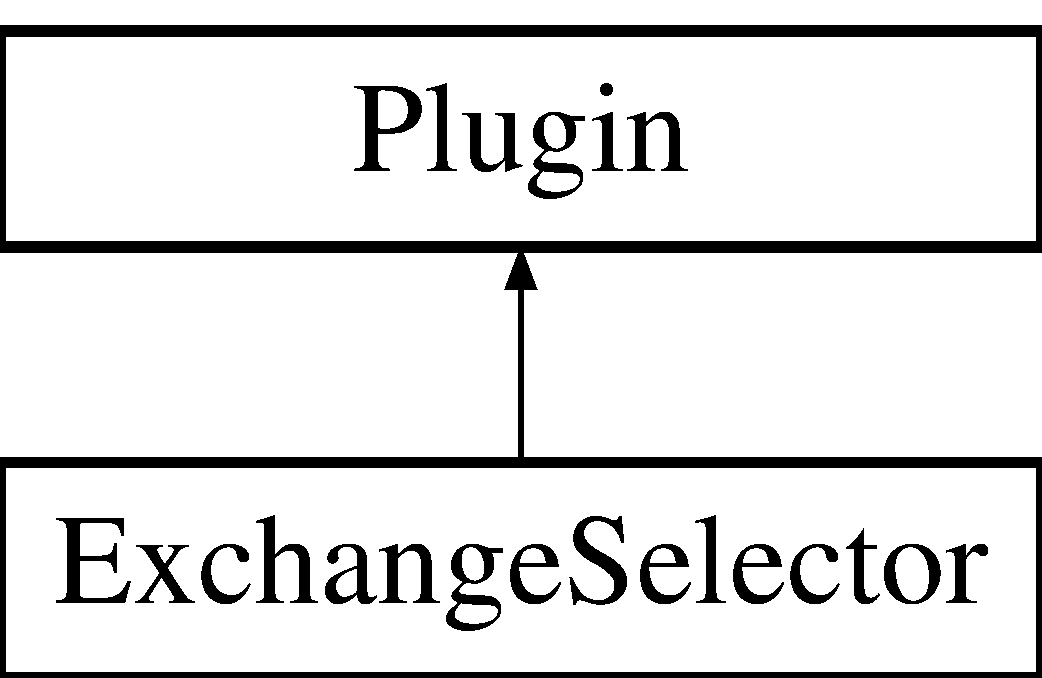
\includegraphics[height=2.000000cm]{d7/da5/classExchangeSelector}
\end{center}
\end{figure}
\subsection*{Public Member Functions}
\begin{DoxyCompactItemize}
\item 
\mbox{\Hypertarget{classExchangeSelector_aaa310ac479ff8a3419e8f2b43e37b5af}\label{classExchangeSelector_aaa310ac479ff8a3419e8f2b43e37b5af}} 
virtual void {\bfseries exchange} (vector$<$ \mbox{\hyperlink{classIndividual}{Individual}} $\ast$$>$ \&migrated, vector$<$ \mbox{\hyperlink{classIndividual}{Individual}} $\ast$$>$ \&population)=0
\end{DoxyCompactItemize}
\subsection*{Additional Inherited Members}


The documentation for this class was generated from the following file\+:\begin{DoxyCompactItemize}
\item 
Exchange\+Selector.\+h\end{DoxyCompactItemize}

\hypertarget{classExecutionIsland}{}\section{Execution\+Island Class Reference}
\label{classExecutionIsland}\index{Execution\+Island@{Execution\+Island}}
\subsection*{Public Member Functions}
\begin{DoxyCompactItemize}
\item 
\mbox{\Hypertarget{classExecutionIsland_a050d1773ab51dc5301e19c06f87d7a53}\label{classExecutionIsland_a050d1773ab51dc5301e19c06f87d7a53}} 
{\bfseries Execution\+Island} (const int slave\+Islands, const \mbox{\hyperlink{classConfiguration}{Configuration}} \&configuration)
\item 
\mbox{\Hypertarget{classExecutionIsland_af6731fdb9aa6e8d2df9657f248a67b90}\label{classExecutionIsland_af6731fdb9aa6e8d2df9657f248a67b90}} 
void {\bfseries run} (const \mbox{\hyperlink{classConfiguration}{Configuration}} \&configuration)
\end{DoxyCompactItemize}
\subsection*{Private Attributes}
\begin{DoxyCompactItemize}
\item 
\mbox{\Hypertarget{classExecutionIsland_aa500ea75fd3fea52722706bb2488f227}\label{classExecutionIsland_aa500ea75fd3fea52722706bb2488f227}} 
M\+P\+I\+\_\+\+Comm {\bfseries execution\+Island\+Comm}
\item 
\mbox{\Hypertarget{classExecutionIsland_a7f4c86eb1145ed9f5f7dd89742cb70df}\label{classExecutionIsland_a7f4c86eb1145ed9f5f7dd89742cb70df}} 
int {\bfseries complete\+Generations}
\item 
\mbox{\Hypertarget{classExecutionIsland_a4c20ae07df9115735a0ec4ecf2ff0ac6}\label{classExecutionIsland_a4c20ae07df9115735a0ec4ecf2ff0ac6}} 
long double $\ast$ {\bfseries buffer}
\item 
\mbox{\Hypertarget{classExecutionIsland_ada43a3c9ef35af66cf1b4ff47bf8bb38}\label{classExecutionIsland_ada43a3c9ef35af66cf1b4ff47bf8bb38}} 
int {\bfseries tam\+Buffer}
\item 
\mbox{\Hypertarget{classExecutionIsland_a6f6c423e8adad0e02034debfdd9809b7}\label{classExecutionIsland_a6f6c423e8adad0e02034debfdd9809b7}} 
int {\bfseries tam\+Buffer2}
\item 
\mbox{\Hypertarget{classExecutionIsland_adb2816efc3f912c4e9506392bbb2c245}\label{classExecutionIsland_adb2816efc3f912c4e9506392bbb2c245}} 
double {\bfseries p\+Migration}
\item 
\mbox{\Hypertarget{classExecutionIsland_a59fce7378b8f455332af34035d959426}\label{classExecutionIsland_a59fce7378b8f455332af34035d959426}} 
unsigned int {\bfseries max\+Ind\+To\+Migrate}
\item 
\mbox{\Hypertarget{classExecutionIsland_a6dae253f6f1faa81853562da936d5f57}\label{classExecutionIsland_a6dae253f6f1faa81853562da936d5f57}} 
unsigned int {\bfseries slave\+Islands}
\item 
\mbox{\Hypertarget{classExecutionIsland_a87b495a9cc15f4792633fe39c2ff8c95}\label{classExecutionIsland_a87b495a9cc15f4792633fe39c2ff8c95}} 
int {\bfseries number\+Of\+Processes\+Per\+Execution}
\item 
\mbox{\Hypertarget{classExecutionIsland_a1dc4a4eb05c2f8dc45f3019983e5815d}\label{classExecutionIsland_a1dc4a4eb05c2f8dc45f3019983e5815d}} 
int {\bfseries my\+Master}
\item 
\mbox{\Hypertarget{classExecutionIsland_a9ff6f54134c1097cd692986525b9991f}\label{classExecutionIsland_a9ff6f54134c1097cd692986525b9991f}} 
int {\bfseries my\+Id}
\item 
\mbox{\Hypertarget{classExecutionIsland_a33caade84ef9e6e5ab390d3f5228f606}\label{classExecutionIsland_a33caade84ef9e6e5ab390d3f5228f606}} 
int {\bfseries num\+Procs}
\item 
\mbox{\Hypertarget{classExecutionIsland_a51f38c60209e6c24be820381fc0a1965}\label{classExecutionIsland_a51f38c60209e6c24be820381fc0a1965}} 
vector$<$ int $>$ {\bfseries my\+Partners}
\item 
\mbox{\Hypertarget{classExecutionIsland_a63fe0b7e697e81a80ff2c3a594d26d02}\label{classExecutionIsland_a63fe0b7e697e81a80ff2c3a594d26d02}} 
map$<$ int, double $\ast$ $>$ {\bfseries configs\+Restart\+Info}
\item 
\mbox{\Hypertarget{classExecutionIsland_abf33ea9f3fcf127db9d6c3d35bb5f811}\label{classExecutionIsland_abf33ea9f3fcf127db9d6c3d35bb5f811}} 
queue$<$ pair$<$ M\+P\+I\+\_\+\+Request $\ast$, long double $\ast$ $>$ $>$ {\bfseries pending\+Requests}
\item 
\mbox{\Hypertarget{classExecutionIsland_ab3b9f3eedc49ae903f502a09bf5a2fde}\label{classExecutionIsland_ab3b9f3eedc49ae903f502a09bf5a2fde}} 
vector$<$ \mbox{\hyperlink{classIndividual}{Individual}} $\ast$ $>$ {\bfseries original\+Population}
\end{DoxyCompactItemize}
\subsection*{Static Private Attributes}
\begin{DoxyCompactItemize}
\item 
\mbox{\Hypertarget{classExecutionIsland_ab6a3bccbb5b13ca7557b49c7204386eb}\label{classExecutionIsland_ab6a3bccbb5b13ca7557b49c7204386eb}} 
static const int {\bfseries D\+E\+F\+\_\+\+S\+I\+Z\+E\+\_\+\+B\+UF} = 10
\end{DoxyCompactItemize}


The documentation for this class was generated from the following files\+:\begin{DoxyCompactItemize}
\item 
Execution\+Island.\+h\item 
Execution\+Island.\+cpp\end{DoxyCompactItemize}

\hypertarget{classGlobalScoreAlgorithm}{}\section{Global\+Score\+Algorithm Class Reference}
\label{classGlobalScoreAlgorithm}\index{Global\+Score\+Algorithm@{Global\+Score\+Algorithm}}
Inheritance diagram for Global\+Score\+Algorithm\+:\begin{figure}[H]
\begin{center}
\leavevmode
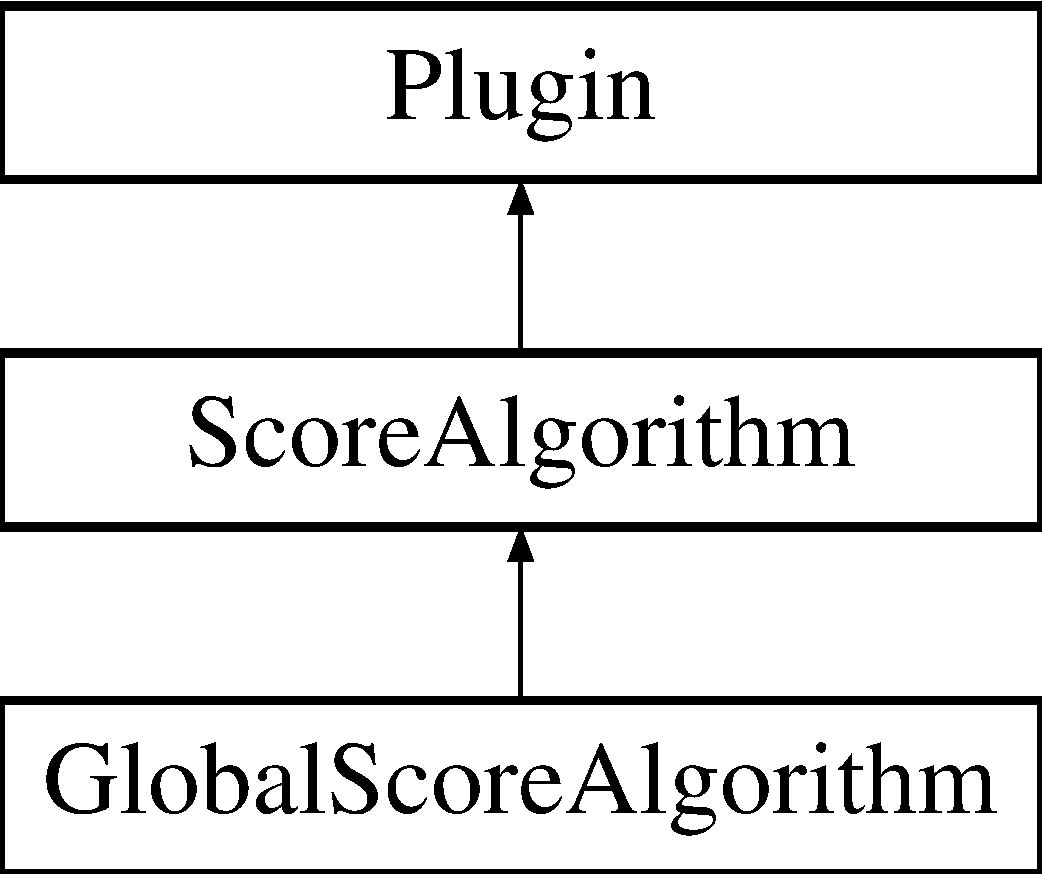
\includegraphics[height=3.000000cm]{d4/dfe/classGlobalScoreAlgorithm}
\end{center}
\end{figure}
\subsection*{Public Member Functions}
\begin{DoxyCompactItemize}
\item 
\mbox{\Hypertarget{classGlobalScoreAlgorithm_a7bb80f3b59672efe3e5b42682c905d8f}\label{classGlobalScoreAlgorithm_a7bb80f3b59672efe3e5b42682c905d8f}} 
virtual long double {\bfseries estimate\+Score} (const int alg, const int conf, const double rnd\+Value)=0
\item 
\mbox{\Hypertarget{classGlobalScoreAlgorithm_a9d746fc68d65fcb9d645d0f8f0a31531}\label{classGlobalScoreAlgorithm_a9d746fc68d65fcb9d645d0f8f0a31531}} 
virtual void {\bfseries update\+Score} (const int alg, const int conf, const \mbox{\hyperlink{classMOFront}{M\+O\+Front}} $\ast$global\+Solution, const int inserted)=0
\item 
\mbox{\Hypertarget{classGlobalScoreAlgorithm_aa97507d258132308eb0a1b9863ee13c5}\label{classGlobalScoreAlgorithm_aa97507d258132308eb0a1b9863ee13c5}} 
virtual long double {\bfseries score} (const \mbox{\hyperlink{classMOFront}{M\+O\+Front}} $\ast$)=0
\end{DoxyCompactItemize}
\subsection*{Additional Inherited Members}


The documentation for this class was generated from the following files\+:\begin{DoxyCompactItemize}
\item 
Global\+Score\+Algorithm.\+h\item 
Global\+Score\+Algorithm.\+cpp\end{DoxyCompactItemize}

\hypertarget{classIndividual}{}\section{Individual Class Reference}
\label{classIndividual}\index{Individual@{Individual}}


Mother class to represent individuals (Problems)  




{\ttfamily \#include $<$Individual.\+h$>$}

Inheritance diagram for Individual\+:\begin{figure}[H]
\begin{center}
\leavevmode
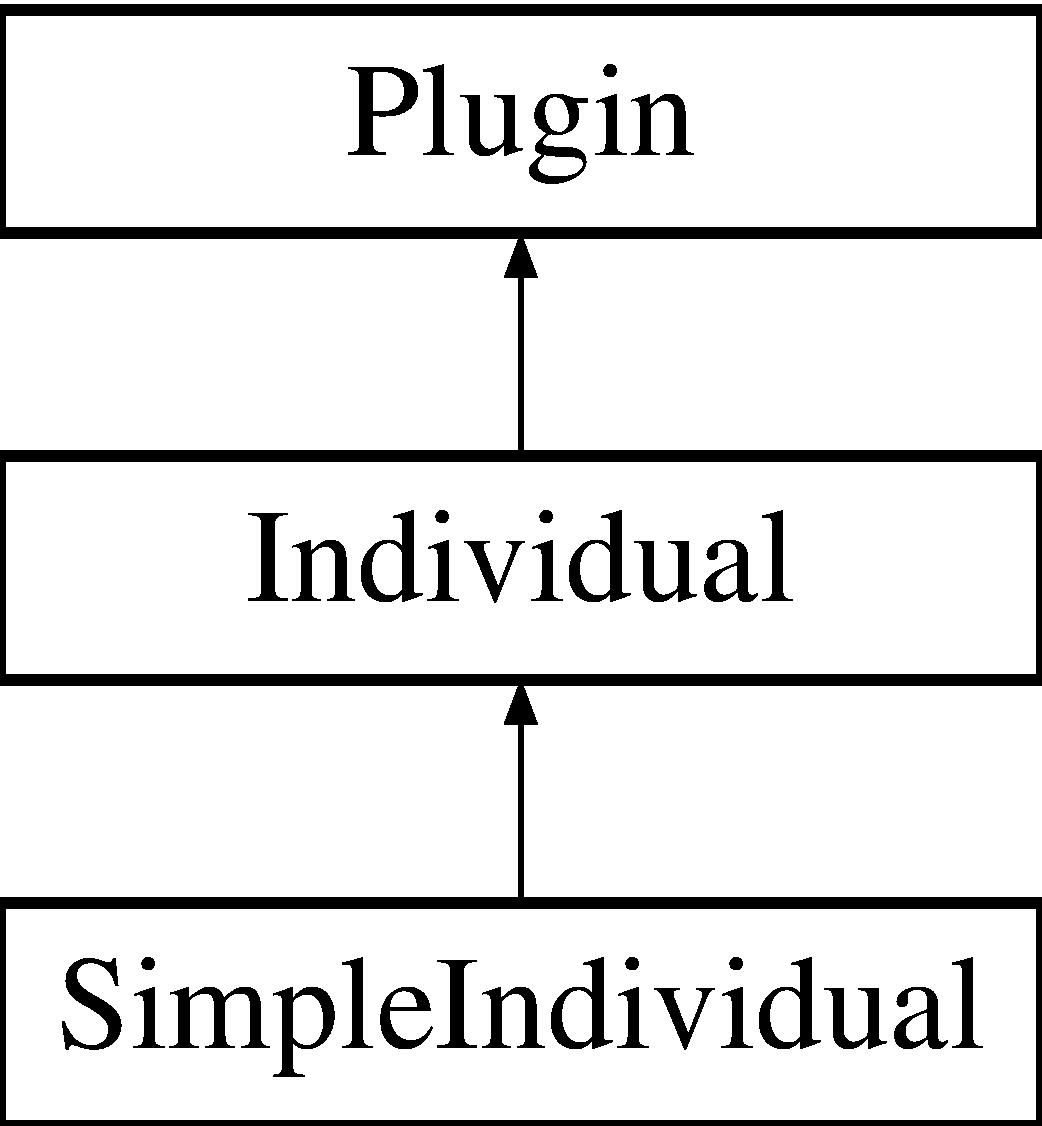
\includegraphics[height=3.000000cm]{d6/d0c/classIndividual}
\end{center}
\end{figure}
\subsection*{Public Member Functions}
\begin{DoxyCompactItemize}
\item 
\mbox{\Hypertarget{classIndividual_a6093773270d0dc49f4bd1d289e8b026e}\label{classIndividual_a6093773270d0dc49f4bd1d289e8b026e}} 
void {\bfseries mutate\+\_\+binary\+\_\+flip} (double pm, int origin=0, int destination=-\/1)
\item 
\mbox{\Hypertarget{classIndividual_a0a08bd4e2c891329f7247f569300c910}\label{classIndividual_a0a08bd4e2c891329f7247f569300c910}} 
void {\bfseries mutate\+\_\+uniform\+\_\+one} (double pm)
\item 
\mbox{\Hypertarget{classIndividual_aa813180f56458071173e34314124dd69}\label{classIndividual_aa813180f56458071173e34314124dd69}} 
void {\bfseries mutate\+\_\+uniform} (double pm, int origin=0, int destination=-\/1)
\item 
\mbox{\Hypertarget{classIndividual_a74bd4e537f04468dd2a1fb76a8135d70}\label{classIndividual_a74bd4e537f04468dd2a1fb76a8135d70}} 
void {\bfseries mutate\+\_\+binary} (double pm)
\item 
\mbox{\Hypertarget{classIndividual_afa9b34ae673b8a7b355cff0e11e2cd3b}\label{classIndividual_afa9b34ae673b8a7b355cff0e11e2cd3b}} 
void {\bfseries mutate\+\_\+range} (double pm)
\item 
\mbox{\Hypertarget{classIndividual_a180da20e7bd49ce2e5950c7ee4e0a304}\label{classIndividual_a180da20e7bd49ce2e5950c7ee4e0a304}} 
void {\bfseries mutate\+\_\+\+Pol} (double pm, int origin=0, int destination=-\/1)
\item 
\mbox{\Hypertarget{classIndividual_a51b40ce43c02e2087c6781f23bd0da3b}\label{classIndividual_a51b40ce43c02e2087c6781f23bd0da3b}} 
void {\bfseries mutate\+\_\+\+Pol2} (double pm, int origin=0, int destination=-\/1)
\item 
\mbox{\Hypertarget{classIndividual_a96b5da395328e11fd60f4fa0af07b2d7}\label{classIndividual_a96b5da395328e11fd60f4fa0af07b2d7}} 
void {\bfseries crossover\+\_\+range} (\mbox{\hyperlink{classIndividual}{Individual}} $\ast$ind, const int interval)
\item 
\mbox{\Hypertarget{classIndividual_a2c454d63a886a6245eee7b1d82284411}\label{classIndividual_a2c454d63a886a6245eee7b1d82284411}} 
void {\bfseries crossover\+\_\+uniform} (\mbox{\hyperlink{classIndividual}{Individual}} $\ast$ind, int origin=0, int destination=-\/1)
\item 
\mbox{\Hypertarget{classIndividual_a0972d982f28d6f51de7cf06ed35a2c1f}\label{classIndividual_a0972d982f28d6f51de7cf06ed35a2c1f}} 
void {\bfseries crossover\+\_\+\+S\+BX} (\mbox{\hyperlink{classIndividual}{Individual}} $\ast$ind, int origin=0, int destination=-\/1)
\item 
\mbox{\Hypertarget{classIndividual_a44928e95dffa8255c21f70d7a906fdb0}\label{classIndividual_a44928e95dffa8255c21f70d7a906fdb0}} 
void {\bfseries crossover\+\_\+\+S\+B\+X2} (\mbox{\hyperlink{classIndividual}{Individual}} $\ast$ind)
\item 
\mbox{\Hypertarget{classIndividual_a7349f4844f5a78a43e6e29d9e701887a}\label{classIndividual_a7349f4844f5a78a43e6e29d9e701887a}} 
void {\bfseries crossover\+\_\+\+O\+PC} (\mbox{\hyperlink{classIndividual}{Individual}} $\ast$ind, int origin=0, int destination=-\/1)
\item 
\mbox{\Hypertarget{classIndividual_a43726fb38d841dd9fcb3e378c258ec06}\label{classIndividual_a43726fb38d841dd9fcb3e378c258ec06}} 
void {\bfseries crossover\+\_\+\+T\+PC} (\mbox{\hyperlink{classIndividual}{Individual}} $\ast$ind, int origin=0, int destination=-\/1)
\item 
\mbox{\Hypertarget{classIndividual_a789500ea4f3299f1482b8ec7f38be9a3}\label{classIndividual_a789500ea4f3299f1482b8ec7f38be9a3}} 
void {\bfseries mutation} (double pm)
\item 
\mbox{\Hypertarget{classIndividual_a5c3c8a3b935c67bdb897410fc42c50c9}\label{classIndividual_a5c3c8a3b935c67bdb897410fc42c50c9}} 
void {\bfseries crossover} (\mbox{\hyperlink{classIndividual}{Individual}} $\ast$ind)
\item 
\mbox{\Hypertarget{classIndividual_a909890a10fad8caedfee75df4e4275a4}\label{classIndividual_a909890a10fad8caedfee75df4e4275a4}} 
void {\bfseries delete\+Vars} ()
\item 
\mbox{\Hypertarget{classIndividual_afe188906f7a4414c1420d81ba77cd19f}\label{classIndividual_afe188906f7a4414c1420d81ba77cd19f}} 
virtual void {\bfseries evaluate} (void)=0
\item 
\mbox{\Hypertarget{classIndividual_a567920f87071ab8bbac7bea9d9ef970f}\label{classIndividual_a567920f87071ab8bbac7bea9d9ef970f}} 
unsigned int {\bfseries get\+Number\+Of\+Var} (void) const
\item 
\mbox{\Hypertarget{classIndividual_a1823a9a02df3bca64cca7b9d67ce39c3}\label{classIndividual_a1823a9a02df3bca64cca7b9d67ce39c3}} 
double {\bfseries get\+Var} (const int i) const
\item 
\mbox{\Hypertarget{classIndividual_a2a88ee53411472e3e91ab5b39e618b23}\label{classIndividual_a2a88ee53411472e3e91ab5b39e618b23}} 
unsigned int {\bfseries get\+Number\+Of\+Obj} (void) const
\item 
\mbox{\Hypertarget{classIndividual_ad867138d74c6f7ed4a40653acbbe564e}\label{classIndividual_ad867138d74c6f7ed4a40653acbbe564e}} 
long double {\bfseries get\+Obj} (const int i) const
\item 
\mbox{\Hypertarget{classIndividual_ac7180dae391a4b76cf7283bb3ae7e0a2}\label{classIndividual_ac7180dae391a4b76cf7283bb3ae7e0a2}} 
unsigned int {\bfseries get\+Number\+Of\+Mig\+Data} (void) const
\item 
\mbox{\Hypertarget{classIndividual_a224a48c2975b1c862bb407a20c329ddb}\label{classIndividual_a224a48c2975b1c862bb407a20c329ddb}} 
unsigned int {\bfseries get\+Number\+Of\+Aux\+Data} (void) const
\item 
\mbox{\Hypertarget{classIndividual_aec4b5a16194cc1cd1d8c98c22ee1033d}\label{classIndividual_aec4b5a16194cc1cd1d8c98c22ee1033d}} 
double {\bfseries get\+Migration\+Data} (const int i) const
\item 
\mbox{\Hypertarget{classIndividual_a915b5251c26d78bbacd3217b5f0cda5a}\label{classIndividual_a915b5251c26d78bbacd3217b5f0cda5a}} 
double {\bfseries get\+Aux\+Data} (const int i) const
\item 
\mbox{\Hypertarget{classIndividual_afaefb518f34a0cee32c8cf9f0105ab09}\label{classIndividual_afaefb518f34a0cee32c8cf9f0105ab09}} 
unsigned int {\bfseries get\+Aux\+Data\+Size} (void) const
\item 
\mbox{\Hypertarget{classIndividual_a4b8c30aeaaf3c718d3ea2d36626dd581}\label{classIndividual_a4b8c30aeaaf3c718d3ea2d36626dd581}} 
double {\bfseries get\+Algorithm\+Data} (const int i) const
\item 
\mbox{\Hypertarget{classIndividual_a5d6f94bfb26b12bb814ae33c41d53171}\label{classIndividual_a5d6f94bfb26b12bb814ae33c41d53171}} 
double {\bfseries get\+Algorithm\+Data\+Size} (void) const
\item 
\mbox{\Hypertarget{classIndividual_acd07ae051e15b48872401de61d888bf3}\label{classIndividual_acd07ae051e15b48872401de61d888bf3}} 
double {\bfseries get\+Fitness\+Value} (void) const
\item 
\mbox{\Hypertarget{classIndividual_a4244c72e717c2bb1bfe78c74768da777}\label{classIndividual_a4244c72e717c2bb1bfe78c74768da777}} 
Owner {\bfseries get\+Owner} (void) const
\item 
\mbox{\Hypertarget{classIndividual_aae95dd48e11039b7e721a221316f929a}\label{classIndividual_aae95dd48e11039b7e721a221316f929a}} 
unsigned int {\bfseries get\+Internal\+Opt\+Direction} (const int i) const
\item 
\mbox{\Hypertarget{classIndividual_afa96281426e0b761c9054475173a53af}\label{classIndividual_afa96281426e0b761c9054475173a53af}} 
virtual double {\bfseries get\+Maximum} (const int i) const =0
\item 
\mbox{\Hypertarget{classIndividual_af40bb21011fa5725d5c81514d8954148}\label{classIndividual_af40bb21011fa5725d5c81514d8954148}} 
virtual double {\bfseries get\+Minimum} (const int i) const =0
\item 
\mbox{\Hypertarget{classIndividual_ac01510009bcdcee97a15c107cfcccbe1}\label{classIndividual_ac01510009bcdcee97a15c107cfcccbe1}} 
\mbox{\hyperlink{classMultiObjectivization}{Multi\+Objectivization}} $\ast$ {\bfseries get\+Multi\+Objectivization\+Plugin} (int index) const
\item 
\mbox{\Hypertarget{classIndividual_aa68afefaff7dac801e0c06a438c31edf}\label{classIndividual_aa68afefaff7dac801e0c06a438c31edf}} 
int {\bfseries get\+Num\+Multi\+Objectivization\+Plugins} (void) const
\item 
\mbox{\Hypertarget{classIndividual_ae3922aadae6b6f49656b9175ec1a6a90}\label{classIndividual_ae3922aadae6b6f49656b9175ec1a6a90}} 
void {\bfseries set\+Obj} (const int i, const long double value)
\item 
\mbox{\Hypertarget{classIndividual_af80f0f301bf71944e44a1336a1d02275}\label{classIndividual_af80f0f301bf71944e44a1336a1d02275}} 
void {\bfseries set\+Var} (const int i, const double value)
\item 
\mbox{\Hypertarget{classIndividual_ad89e179d02713b647f751c73a5cd5978}\label{classIndividual_ad89e179d02713b647f751c73a5cd5978}} 
void {\bfseries set\+Fitness\+Value} (const double value)
\item 
\mbox{\Hypertarget{classIndividual_ad51b2cd41c4370b7b834b5f71ec18a09}\label{classIndividual_ad51b2cd41c4370b7b834b5f71ec18a09}} 
void {\bfseries set\+Migration\+Data} (const int i, const double value)
\item 
\mbox{\Hypertarget{classIndividual_a82d3c3228f08e7b13469946fe6f4b6c4}\label{classIndividual_a82d3c3228f08e7b13469946fe6f4b6c4}} 
void {\bfseries set\+Aux\+Data} (const int i, const double value)
\item 
\mbox{\Hypertarget{classIndividual_a632f3937b6a074eba85cb268e13cf98c}\label{classIndividual_a632f3937b6a074eba85cb268e13cf98c}} 
void {\bfseries set\+Number\+Of\+Var} (const int n)
\item 
\mbox{\Hypertarget{classIndividual_a57b610304fdb2b7ef442c287472df7dc}\label{classIndividual_a57b610304fdb2b7ef442c287472df7dc}} 
void {\bfseries set\+Number\+Of\+Obj} (const int n)
\item 
\mbox{\Hypertarget{classIndividual_a34e31746ea41d0dfae4e780175e227ec}\label{classIndividual_a34e31746ea41d0dfae4e780175e227ec}} 
void {\bfseries set\+Algorithm\+Data} (const int i, const double value)
\item 
\mbox{\Hypertarget{classIndividual_afcee9a2a14bce879233127de7052c04d}\label{classIndividual_afcee9a2a14bce879233127de7052c04d}} 
void {\bfseries set\+Aux\+Data\+Size} (const int n)
\item 
\mbox{\Hypertarget{classIndividual_af5b4c849207df6d0633f4860af0c3cd1}\label{classIndividual_af5b4c849207df6d0633f4860af0c3cd1}} 
void {\bfseries set\+Migration\+Data\+Size} (const int n)
\item 
\mbox{\Hypertarget{classIndividual_ab562578d64333b00ccd0e20fd079e3d2}\label{classIndividual_ab562578d64333b00ccd0e20fd079e3d2}} 
void {\bfseries set\+Owner} (const Owner own)
\item 
\mbox{\Hypertarget{classIndividual_a5176a4131d6bceb7e84280f84a623ff0}\label{classIndividual_a5176a4131d6bceb7e84280f84a623ff0}} 
void {\bfseries set\+Mut\+Operator} (\mbox{\hyperlink{classMutation}{Mutation}} $\ast$mut)
\item 
\mbox{\Hypertarget{classIndividual_a790e135b019ce331cb9e1270193c3313}\label{classIndividual_a790e135b019ce331cb9e1270193c3313}} 
void {\bfseries set\+Cross\+Operator} (\mbox{\hyperlink{classCrossover}{Crossover}} $\ast$cross)
\item 
\mbox{\Hypertarget{classIndividual_ac9d4ad0bf7bd5bebbc6e13bc2090bfea}\label{classIndividual_ac9d4ad0bf7bd5bebbc6e13bc2090bfea}} 
void {\bfseries set\+Multi\+Objectivization\+Plugins} (const vector$<$ \mbox{\hyperlink{classMultiObjectivization}{Multi\+Objectivization}} $\ast$$>$ \&multi)
\item 
\mbox{\Hypertarget{classIndividual_ac51b9b06ff8b7ad2b8b3e3138e53e875}\label{classIndividual_ac51b9b06ff8b7ad2b8b3e3138e53e875}} 
int {\bfseries request\+Algorithm\+Data} (void)
\item 
\mbox{\Hypertarget{classIndividual_af97490ce47977903aaf34b6af0d8c410}\label{classIndividual_af97490ce47977903aaf34b6af0d8c410}} 
void {\bfseries release\+Algorithm\+Data} (void)
\item 
\mbox{\Hypertarget{classIndividual_a519dab6ca141dd139a0676c8f27e5e98}\label{classIndividual_a519dab6ca141dd139a0676c8f27e5e98}} 
\mbox{\hyperlink{classIndividual}{Individual}} $\ast$ {\bfseries internal\+Clone} (void) const
\item 
\mbox{\Hypertarget{classIndividual_aadc2d0ee76ca08335739faddde118888}\label{classIndividual_aadc2d0ee76ca08335739faddde118888}} 
void {\bfseries internal\+Clone} (const \mbox{\hyperlink{classIndividual}{Individual}} $\ast$)
\item 
\mbox{\Hypertarget{classIndividual_a1fa420271445d3c72cf1c498dc4a990f}\label{classIndividual_a1fa420271445d3c72cf1c498dc4a990f}} 
void {\bfseries internal\+Clone\+Data} (const \mbox{\hyperlink{classIndividual}{Individual}} $\ast$)
\item 
\mbox{\Hypertarget{classIndividual_ab2365dcac4b47bca82a0631c6e2d3a3d}\label{classIndividual_ab2365dcac4b47bca82a0631c6e2d3a3d}} 
void {\bfseries serialize} (long double $\ast$buffer, int \&count) const
\item 
\mbox{\Hypertarget{classIndividual_a25eb4ad558ab7d35a6d26b4f9aa05773}\label{classIndividual_a25eb4ad558ab7d35a6d26b4f9aa05773}} 
\mbox{\hyperlink{classIndividual}{Individual}} $\ast$ {\bfseries deserialize} (const int n\+Var, const int n\+Obj, const int n\+Mig, const long double $\ast$buffer, int \&count)
\item 
\mbox{\Hypertarget{classIndividual_acb2d52f3e74da456e367bc375f9d5c4f}\label{classIndividual_acb2d52f3e74da456e367bc375f9d5c4f}} 
virtual void {\bfseries deserialized} ()
\item 
\mbox{\Hypertarget{classIndividual_a4ca04ade73ff56a0d729d11435a5d519}\label{classIndividual_a4ca04ade73ff56a0d729d11435a5d519}} 
virtual void {\bfseries cloned} ()
\item 
\mbox{\Hypertarget{classIndividual_a1f6b80956eafdd5fa33a6224b96b2e07}\label{classIndividual_a1f6b80956eafdd5fa33a6224b96b2e07}} 
virtual void {\bfseries maintain\+Only\+Obj} ()
\item 
\mbox{\Hypertarget{classIndividual_af8b73dad774466aed120ff2126459d3e}\label{classIndividual_af8b73dad774466aed120ff2126459d3e}} 
void {\bfseries maintain\+Only\+Obj\+Internal} ()
\item 
\mbox{\Hypertarget{classIndividual_a6aabda914856d6384997d7dbc04981af}\label{classIndividual_a6aabda914856d6384997d7dbc04981af}} 
virtual void {\bfseries print} (ostream \&os) const
\item 
\mbox{\Hypertarget{classIndividual_a35fae68fdf132bc32e343104cc0c35d3}\label{classIndividual_a35fae68fdf132bc32e343104cc0c35d3}} 
virtual void {\bfseries print\+Info} (ostream \&os) const
\item 
\mbox{\Hypertarget{classIndividual_a5175fb96632db18a74010297036c35e6}\label{classIndividual_a5175fb96632db18a74010297036c35e6}} 
virtual string {\bfseries get\+Mutation\+Name} () const
\item 
\mbox{\Hypertarget{classIndividual_a1236414e5aaf1f419409f11c5ee37540}\label{classIndividual_a1236414e5aaf1f419409f11c5ee37540}} 
virtual int {\bfseries get\+Mutation\+Number\+Of\+Parameters} () const
\item 
\mbox{\Hypertarget{classIndividual_a2bfbdc16b00ac7a4fcf9ea28ff0523a7}\label{classIndividual_a2bfbdc16b00ac7a4fcf9ea28ff0523a7}} 
virtual string {\bfseries get\+Mutation\+Parameter\+Name} (int i) const
\item 
\mbox{\Hypertarget{classIndividual_ade6c76311ce0011385b1214d9e4b536f}\label{classIndividual_ade6c76311ce0011385b1214d9e4b536f}} 
virtual string {\bfseries get\+Mutation\+Parameter\+Value} (int i) const
\item 
\mbox{\Hypertarget{classIndividual_ad9c6819d323fecfc4ded5aeb7f77648b}\label{classIndividual_ad9c6819d323fecfc4ded5aeb7f77648b}} 
virtual string {\bfseries get\+Crossover\+Name} () const
\item 
\mbox{\Hypertarget{classIndividual_a4bcaad1c9d070d8e3ed1d785356300f3}\label{classIndividual_a4bcaad1c9d070d8e3ed1d785356300f3}} 
virtual int {\bfseries get\+Crossover\+Number\+Of\+Parameters} () const
\item 
\mbox{\Hypertarget{classIndividual_af3058a71a41ed3e8d69bb4367bb1a253}\label{classIndividual_af3058a71a41ed3e8d69bb4367bb1a253}} 
virtual string {\bfseries get\+Crossover\+Parameter\+Name} (int i) const
\item 
\mbox{\Hypertarget{classIndividual_a612d62952361ec165e357be978f9cdcc}\label{classIndividual_a612d62952361ec165e357be978f9cdcc}} 
virtual string {\bfseries get\+Crossover\+Parameter\+Value} (int i) const
\item 
\mbox{\Hypertarget{classIndividual_a212e273f5aa7f6bf7b043f2aaf6d4180}\label{classIndividual_a212e273f5aa7f6bf7b043f2aaf6d4180}} 
virtual string {\bfseries get\+Obj\+Name} (int i) const
\item 
\mbox{\Hypertarget{classIndividual_aa358ac2b049a05d22a691e26af9c115a}\label{classIndividual_aa358ac2b049a05d22a691e26af9c115a}} 
virtual int {\bfseries get\+Index\+Obj} () const
\item 
\mbox{\Hypertarget{classIndividual_a047d5d9c3ce6e26d66c3787242505e8c}\label{classIndividual_a047d5d9c3ce6e26d66c3787242505e8c}} 
virtual int {\bfseries get\+Index\+Obj\+Min} () const
\item 
\mbox{\Hypertarget{classIndividual_a9aa0f5e4ab31fa455876ce2141f3eb1b}\label{classIndividual_a9aa0f5e4ab31fa455876ce2141f3eb1b}} 
virtual int {\bfseries get\+Index\+Obj\+Max} () const
\item 
\mbox{\Hypertarget{classIndividual_a006daae48f79e41b9791fe5b758c9daa}\label{classIndividual_a006daae48f79e41b9791fe5b758c9daa}} 
bool {\bfseries operator$<$} (const \mbox{\hyperlink{classIndividual}{Individual}} \&ind) const
\item 
\mbox{\Hypertarget{classIndividual_ac9ccea2310285f2ea4a5be59013cba96}\label{classIndividual_ac9ccea2310285f2ea4a5be59013cba96}} 
bool {\bfseries operator==} (const \mbox{\hyperlink{classIndividual}{Individual}} \&ind) const
\item 
\mbox{\Hypertarget{classIndividual_ac508a6fa28504a55ca5ab977d5973926}\label{classIndividual_ac508a6fa28504a55ca5ab977d5973926}} 
virtual void {\bfseries restart} (void)
\item 
\mbox{\Hypertarget{classIndividual_aed35f077fddffa3108543fd9b7712062}\label{classIndividual_aed35f077fddffa3108543fd9b7712062}} 
virtual void {\bfseries generation\+Code} () const
\item 
\mbox{\Hypertarget{classIndividual_a9929b4df4addf089ffecc4d697bab527}\label{classIndividual_a9929b4df4addf089ffecc4d697bab527}} 
double {\bfseries get\+Euclidean\+Distance} (const \mbox{\hyperlink{classIndividual}{Individual}} $\ast$) const
\item 
\mbox{\Hypertarget{classIndividual_aca330827f8d265b2b7d5621078678543}\label{classIndividual_aca330827f8d265b2b7d5621078678543}} 
double {\bfseries get\+Euclidean\+Distance\+Decision\+Space} (const \mbox{\hyperlink{classIndividual}{Individual}} $\ast$) const
\item 
\mbox{\Hypertarget{classIndividual_acbfdc03b91966684a6e2e16c11636925}\label{classIndividual_acbfdc03b91966684a6e2e16c11636925}} 
virtual unsigned int {\bfseries get\+Neighbourhood\+Size} () const
\item 
\mbox{\Hypertarget{classIndividual_a5c5cf3b61e16a4ee651bb88107bfc442}\label{classIndividual_a5c5cf3b61e16a4ee651bb88107bfc442}} 
virtual \mbox{\hyperlink{classIndividual}{Individual}} $\ast$ {\bfseries get\+Neighbour} (const int i) const
\item 
\mbox{\Hypertarget{classIndividual_a34c5cb1f96882ac12fdabf5d52ae817d}\label{classIndividual_a34c5cb1f96882ac12fdabf5d52ae817d}} 
virtual void {\bfseries get\+Neighbour\+Objectives} (const int i, vector$<$ double $>$ \&objectives) const
\item 
\mbox{\Hypertarget{classIndividual_a35a32b6e984bff3a162cefe296a30efa}\label{classIndividual_a35a32b6e984bff3a162cefe296a30efa}} 
virtual unsigned int {\bfseries get\+Opt\+Direction} (const int i) const =0
\end{DoxyCompactItemize}
\subsection*{Private Member Functions}
\begin{DoxyCompactItemize}
\item 
\mbox{\Hypertarget{classIndividual_af4553d2ba5e943258c1389735d5caa87}\label{classIndividual_af4553d2ba5e943258c1389735d5caa87}} 
virtual \mbox{\hyperlink{classIndividual}{Individual}} $\ast$ {\bfseries clone} (void) const =0
\item 
\mbox{\Hypertarget{classIndividual_afa6573583c7cebb4a71c09d8e0639048}\label{classIndividual_afa6573583c7cebb4a71c09d8e0639048}} 
virtual void {\bfseries dependent\+Mutation} (double pm)
\item 
\mbox{\Hypertarget{classIndividual_acddee962ce99dcba006c0111c65b26e1}\label{classIndividual_acddee962ce99dcba006c0111c65b26e1}} 
virtual void {\bfseries dependent\+Crossover} (\mbox{\hyperlink{classIndividual}{Individual}} $\ast$ind)
\end{DoxyCompactItemize}
\subsection*{Private Attributes}
\begin{DoxyCompactItemize}
\item 
\mbox{\Hypertarget{classIndividual_a3a418fa4c1acb6d9b470bae8ae4f765b}\label{classIndividual_a3a418fa4c1acb6d9b470bae8ae4f765b}} 
vector$<$ \mbox{\hyperlink{classMultiObjectivization}{Multi\+Objectivization}} $\ast$ $>$ {\bfseries multi\+Objectivizations\+Plugins}
\item 
\mbox{\Hypertarget{classIndividual_a3422766f76333dc26094622a2507f2c5}\label{classIndividual_a3422766f76333dc26094622a2507f2c5}} 
vector$<$ double $>$ {\bfseries var}
\item 
\mbox{\Hypertarget{classIndividual_aeaea908497019d83d1faeb1b14b24806}\label{classIndividual_aeaea908497019d83d1faeb1b14b24806}} 
vector$<$ long double $>$ {\bfseries obj}
\item 
\mbox{\Hypertarget{classIndividual_a52f5c8cae2417f71793bb62a2149159e}\label{classIndividual_a52f5c8cae2417f71793bb62a2149159e}} 
vector$<$ double $>$ {\bfseries migration\+Data}
\item 
\mbox{\Hypertarget{classIndividual_acb44f6c44e7f7c958b9f87172c1864e1}\label{classIndividual_acb44f6c44e7f7c958b9f87172c1864e1}} 
vector$<$ double $>$ {\bfseries aux\+Data}
\item 
\mbox{\Hypertarget{classIndividual_a7d2478a023c6de2d9d16dbd49af196b0}\label{classIndividual_a7d2478a023c6de2d9d16dbd49af196b0}} 
vector$<$ double $>$ {\bfseries algorithm\+Data}
\item 
\mbox{\Hypertarget{classIndividual_adfe2e2d7b2f06dc4721f0a13c9b705af}\label{classIndividual_adfe2e2d7b2f06dc4721f0a13c9b705af}} 
double {\bfseries fitness\+Value}
\item 
\mbox{\Hypertarget{classIndividual_a0cc18b1635d07e4d5c09541cfd4fffa4}\label{classIndividual_a0cc18b1635d07e4d5c09541cfd4fffa4}} 
\mbox{\hyperlink{classMutation}{Mutation}} $\ast$ {\bfseries mut\+Operator}
\item 
\mbox{\Hypertarget{classIndividual_a9c3141911458653cfb75073a51d08dc5}\label{classIndividual_a9c3141911458653cfb75073a51d08dc5}} 
\mbox{\hyperlink{classCrossover}{Crossover}} $\ast$ {\bfseries cross\+Operator}
\item 
\mbox{\Hypertarget{classIndividual_aa65e054afcae994f99941559260f74f9}\label{classIndividual_aa65e054afcae994f99941559260f74f9}} 
Owner {\bfseries owner}
\end{DoxyCompactItemize}
\subsection*{Additional Inherited Members}


\subsection{Detailed Description}
Mother class to represent individuals (Problems) 

The documentation for this class was generated from the following files\+:\begin{DoxyCompactItemize}
\item 
Individual.\+h\item 
Individual.\+cpp\end{DoxyCompactItemize}

\hypertarget{classInitPopIslandLoader}{}\section{Init\+Pop\+Island\+Loader Class Reference}
\label{classInitPopIslandLoader}\index{Init\+Pop\+Island\+Loader@{Init\+Pop\+Island\+Loader}}
Inheritance diagram for Init\+Pop\+Island\+Loader\+:\begin{figure}[H]
\begin{center}
\leavevmode
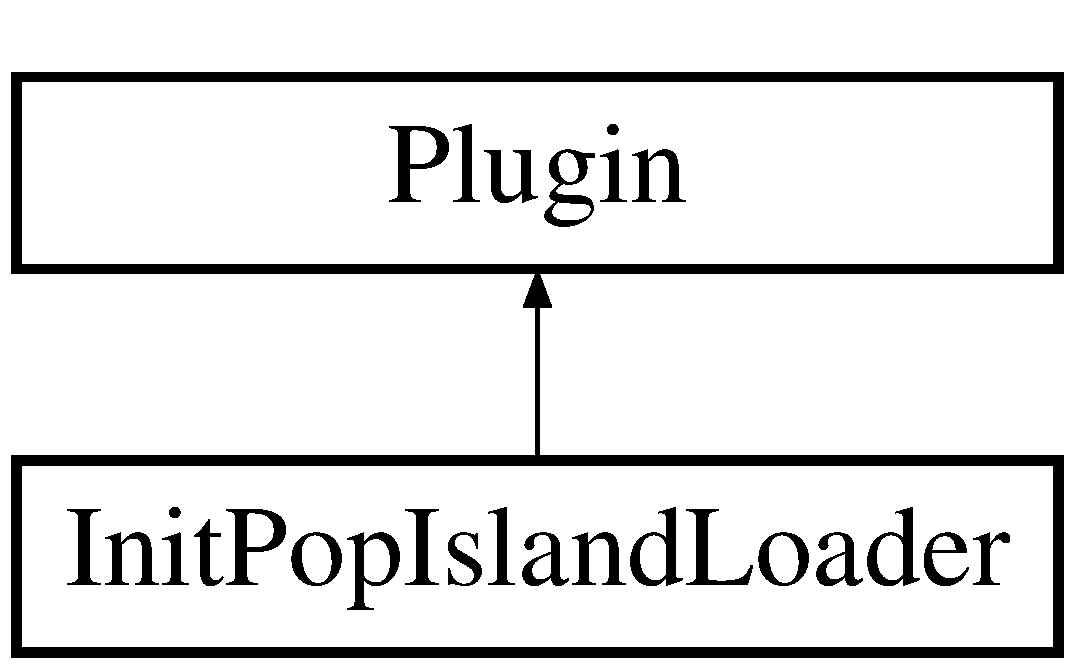
\includegraphics[height=2.000000cm]{d5/da6/classInitPopIslandLoader}
\end{center}
\end{figure}
\subsection*{Public Member Functions}
\begin{DoxyCompactItemize}
\item 
\mbox{\Hypertarget{classInitPopIslandLoader_ad8935d4f5f2eadf3a5a212874f12f784}\label{classInitPopIslandLoader_ad8935d4f5f2eadf3a5a212874f12f784}} 
virtual void {\bfseries load\+Island\+Init\+Pop} (const int previous\+Alg, const int previous\+Conf, const int new\+Alg, const int new\+Conf, const vector$<$ \mbox{\hyperlink{classIndividual}{Individual}} $\ast$ $>$ $\ast$previous\+Init, const vector$<$ \mbox{\hyperlink{classIndividual}{Individual}} $\ast$ $>$ $\ast$previous\+End, const vector$<$ \mbox{\hyperlink{classIndividual}{Individual}} $\ast$ $>$ $\ast$global, vector$<$ \mbox{\hyperlink{classIndividual}{Individual}} $\ast$ $>$ \&new\+Population, vector$<$ int $>$ \&origin) const =0
\item 
\mbox{\Hypertarget{classInitPopIslandLoader_a73b8d540a41a99c7ae0c5de1a7bf23bf}\label{classInitPopIslandLoader_a73b8d540a41a99c7ae0c5de1a7bf23bf}} 
virtual bool {\bfseries use\+Previous\+Init} () const
\item 
\mbox{\Hypertarget{classInitPopIslandLoader_a1025015ccb1d952bbcd421f3eb126814}\label{classInitPopIslandLoader_a1025015ccb1d952bbcd421f3eb126814}} 
virtual bool {\bfseries use\+Previous\+End} () const
\item 
\mbox{\Hypertarget{classInitPopIslandLoader_ad06e23f020118b4a627720b83a1a4323}\label{classInitPopIslandLoader_ad06e23f020118b4a627720b83a1a4323}} 
virtual bool {\bfseries use\+Global} () const
\end{DoxyCompactItemize}
\subsection*{Additional Inherited Members}


The documentation for this class was generated from the following file\+:\begin{DoxyCompactItemize}
\item 
Init\+Pop\+Island\+Loader.\+h\end{DoxyCompactItemize}

\hypertarget{classLocalScoreAlgorithm}{}\section{Local\+Score\+Algorithm Class Reference}
\label{classLocalScoreAlgorithm}\index{Local\+Score\+Algorithm@{Local\+Score\+Algorithm}}
Inheritance diagram for Local\+Score\+Algorithm\+:\begin{figure}[H]
\begin{center}
\leavevmode
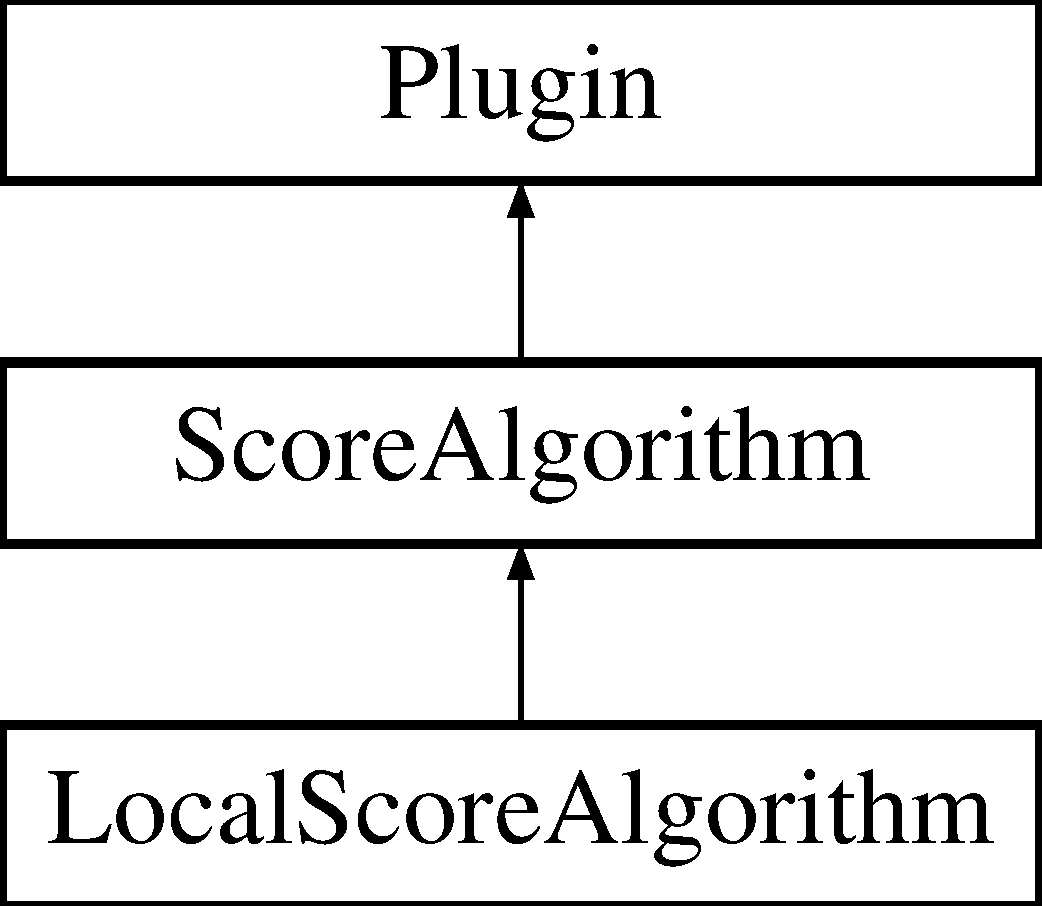
\includegraphics[height=3.000000cm]{d9/db8/classLocalScoreAlgorithm}
\end{center}
\end{figure}
\subsection*{Public Member Functions}
\begin{DoxyCompactItemize}
\item 
\mbox{\Hypertarget{classLocalScoreAlgorithm_a16f56a8b9b2dc36c8b82865327433f4c}\label{classLocalScoreAlgorithm_a16f56a8b9b2dc36c8b82865327433f4c}} 
virtual long double {\bfseries score} (\mbox{\hyperlink{classMOFront}{M\+O\+Front}} $\ast$)=0
\item 
\mbox{\Hypertarget{classLocalScoreAlgorithm_a06854361c6bcfa18fe9ac1bf6c6f62d0}\label{classLocalScoreAlgorithm_a06854361c6bcfa18fe9ac1bf6c6f62d0}} 
virtual void {\bfseries update\+Score} (const long double break\+From, const long double arrive\+To, int alg, int conf, int island\+Id)=0
\item 
\mbox{\Hypertarget{classLocalScoreAlgorithm_a836a125f777298457ee9ae43c990b3fb}\label{classLocalScoreAlgorithm_a836a125f777298457ee9ae43c990b3fb}} 
virtual long double {\bfseries estimate\+Score} (const long double break\+From\+Score, const int alg, const int conf, const int island\+Id, const double rnd\+Value)=0
\end{DoxyCompactItemize}
\subsection*{Additional Inherited Members}


The documentation for this class was generated from the following files\+:\begin{DoxyCompactItemize}
\item 
Local\+Score\+Algorithm.\+h\item 
Local\+Score\+Algorithm.\+cpp\end{DoxyCompactItemize}

\hypertarget{classLocalSearch}{}\section{Local\+Search Class Reference}
\label{classLocalSearch}\index{Local\+Search@{Local\+Search}}
Inheritance diagram for Local\+Search\+:\begin{figure}[H]
\begin{center}
\leavevmode
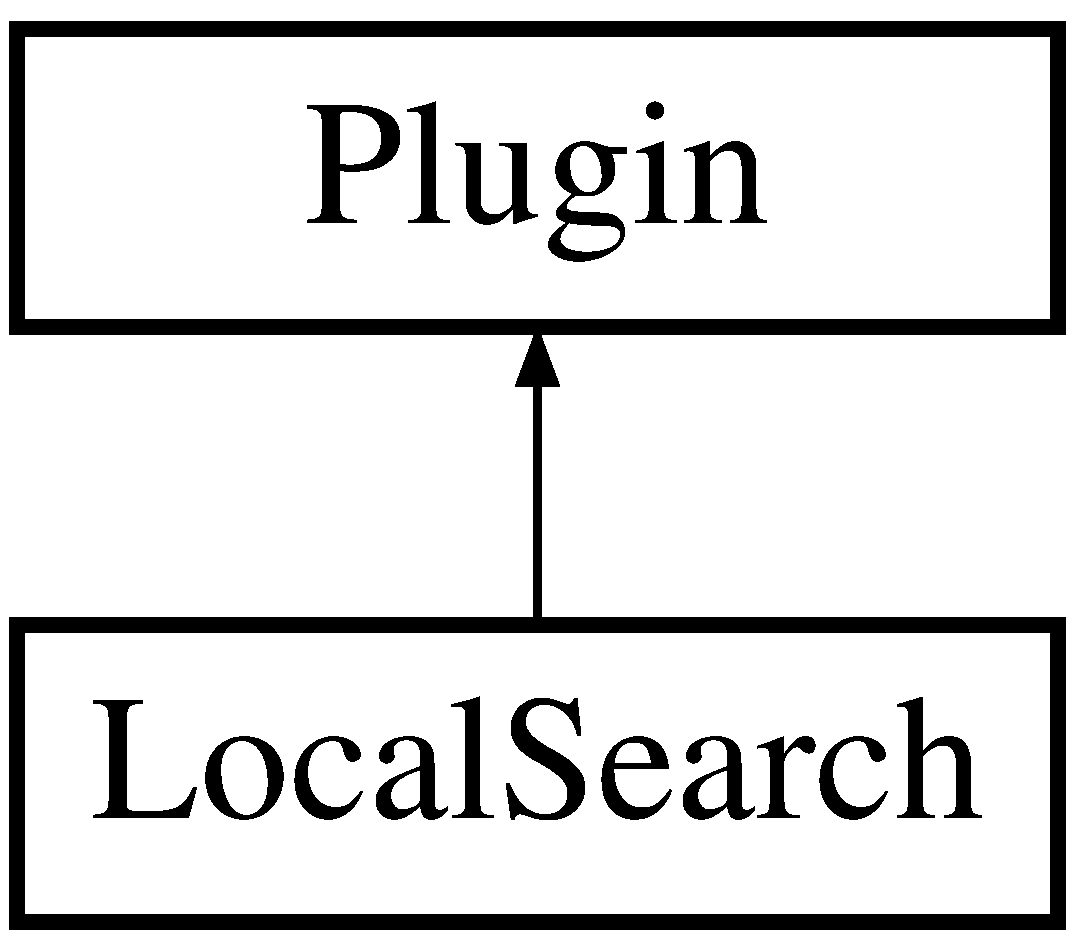
\includegraphics[height=2.000000cm]{d9/d56/classLocalSearch}
\end{center}
\end{figure}
\subsection*{Public Member Functions}
\begin{DoxyCompactItemize}
\item 
\mbox{\Hypertarget{classLocalSearch_a2b6d7b6455c6773c84e5f5a666870b42}\label{classLocalSearch_a2b6d7b6455c6773c84e5f5a666870b42}} 
virtual void {\bfseries local\+Search} (vector$<$ \mbox{\hyperlink{classIndividual}{Individual}} $\ast$$>$ $\ast$population, \mbox{\hyperlink{classMOFront}{M\+O\+Front}} $\ast$current\+Solution)=0
\end{DoxyCompactItemize}
\subsection*{Additional Inherited Members}


The documentation for this class was generated from the following file\+:\begin{DoxyCompactItemize}
\item 
Local\+Search.\+h\end{DoxyCompactItemize}

\hypertarget{classMigrationSelector}{}\section{Migration\+Selector Class Reference}
\label{classMigrationSelector}\index{Migration\+Selector@{Migration\+Selector}}
Inheritance diagram for Migration\+Selector\+:\begin{figure}[H]
\begin{center}
\leavevmode
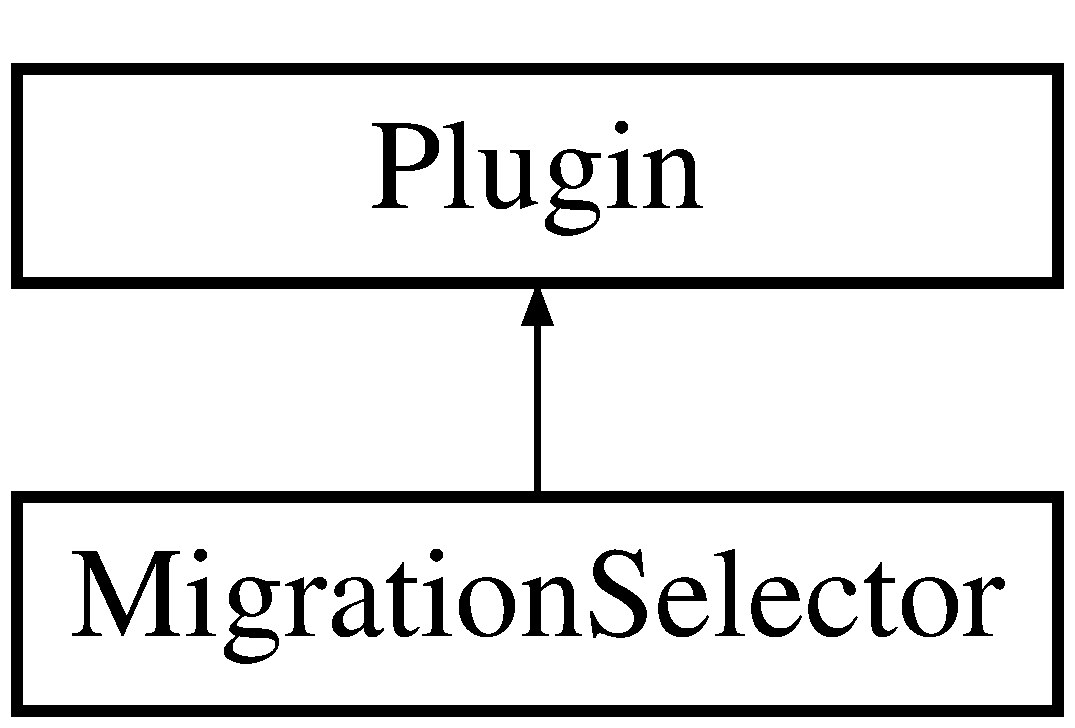
\includegraphics[height=2.000000cm]{d9/d33/classMigrationSelector}
\end{center}
\end{figure}
\subsection*{Public Member Functions}
\begin{DoxyCompactItemize}
\item 
\mbox{\Hypertarget{classMigrationSelector_a1257aad41c61a0e3aa5e902a816a5a9d}\label{classMigrationSelector_a1257aad41c61a0e3aa5e902a816a5a9d}} 
{\bfseries Migration\+Selector} (int type)
\item 
\mbox{\Hypertarget{classMigrationSelector_a5d5f69c022b4a082af7f661ee89c9459}\label{classMigrationSelector_a5d5f69c022b4a082af7f661ee89c9459}} 
int {\bfseries get\+Type} () const
\item 
\mbox{\Hypertarget{classMigrationSelector_a471dfd19b550c5436979439fda76e9f1}\label{classMigrationSelector_a471dfd19b550c5436979439fda76e9f1}} 
virtual void {\bfseries select} (const vector$<$ \mbox{\hyperlink{classIndividual}{Individual}} $\ast$$>$ \&pop, int number\+Individual, vector$<$ int $>$ \&selected)=0
\end{DoxyCompactItemize}
\subsection*{Private Attributes}
\begin{DoxyCompactItemize}
\item 
\mbox{\Hypertarget{classMigrationSelector_a91a77888e27312353fd442e6c59641db}\label{classMigrationSelector_a91a77888e27312353fd442e6c59641db}} 
int {\bfseries type}
\end{DoxyCompactItemize}
\subsection*{Additional Inherited Members}


The documentation for this class was generated from the following files\+:\begin{DoxyCompactItemize}
\item 
Migration\+Selector.\+h\item 
Migration\+Selector.\+cpp\end{DoxyCompactItemize}

\hypertarget{classMigrationTopology}{}\section{Migration\+Topology Class Reference}
\label{classMigrationTopology}\index{Migration\+Topology@{Migration\+Topology}}
Inheritance diagram for Migration\+Topology\+:\begin{figure}[H]
\begin{center}
\leavevmode
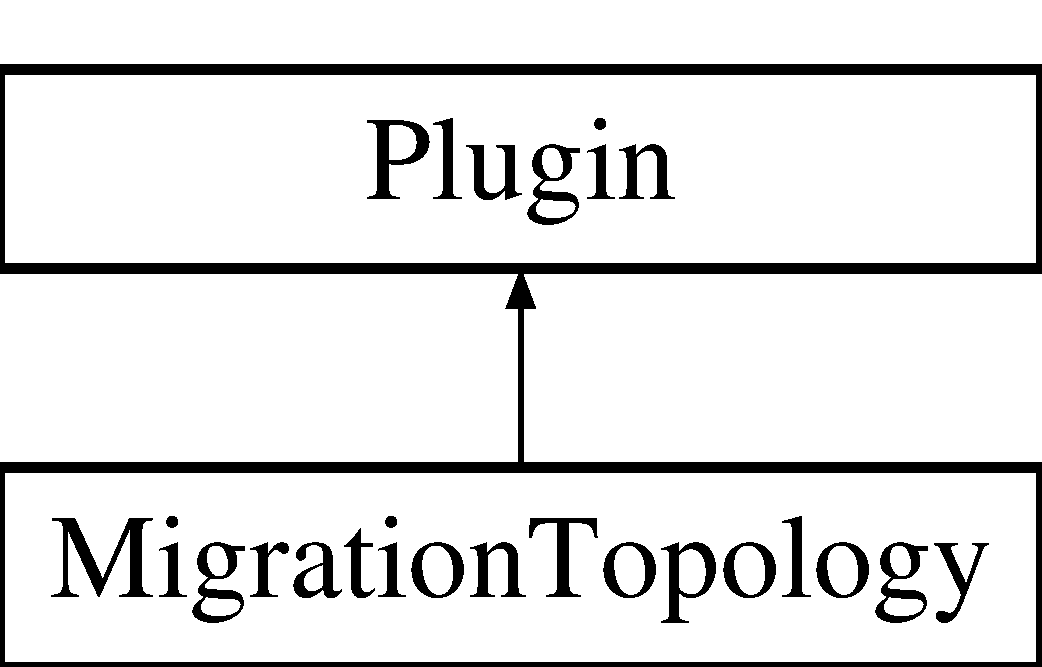
\includegraphics[height=2.000000cm]{d8/d7a/classMigrationTopology}
\end{center}
\end{figure}
\subsection*{Public Member Functions}
\begin{DoxyCompactItemize}
\item 
\mbox{\Hypertarget{classMigrationTopology_a42c2391ef6355880a308ef98beb7273b}\label{classMigrationTopology_a42c2391ef6355880a308ef98beb7273b}} 
virtual void {\bfseries send\+To} (const int my\+Id, const int slave\+Islands, vector$<$ int $>$ \&destination)=0
\end{DoxyCompactItemize}
\subsection*{Additional Inherited Members}


The documentation for this class was generated from the following file\+:\begin{DoxyCompactItemize}
\item 
Migration\+Topology.\+h\end{DoxyCompactItemize}

\hypertarget{classMOFront}{}\section{M\+O\+Front Class Reference}
\label{classMOFront}\index{M\+O\+Front@{M\+O\+Front}}
Inheritance diagram for M\+O\+Front\+:\begin{figure}[H]
\begin{center}
\leavevmode
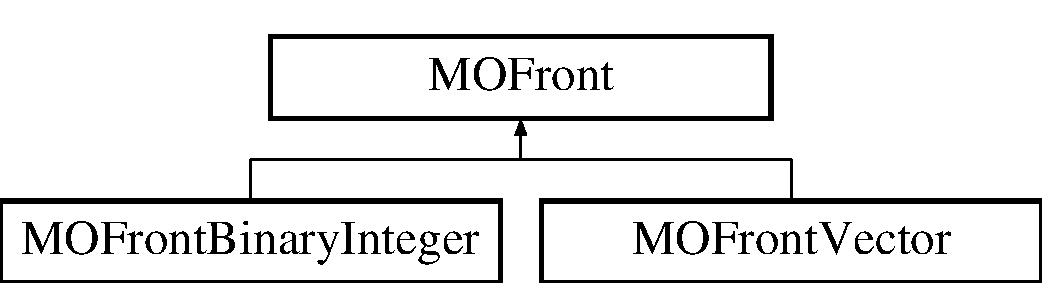
\includegraphics[height=2.000000cm]{d6/d3e/classMOFront}
\end{center}
\end{figure}
\subsection*{Public Member Functions}
\begin{DoxyCompactItemize}
\item 
\mbox{\Hypertarget{classMOFront_acdf484ed4e10a203ade8c6d46e5231db}\label{classMOFront_acdf484ed4e10a203ade8c6d46e5231db}} 
{\bfseries M\+O\+Front} (const \mbox{\hyperlink{classIndividual}{Individual}} $\ast$ej\+Ind, bool copy\+On\+Insert, bool delete\+On\+Destroy)
\item 
\mbox{\Hypertarget{classMOFront_a27a75fdcbdebcce00eb7e7cf841be0ee}\label{classMOFront_a27a75fdcbdebcce00eb7e7cf841be0ee}} 
virtual unsigned int {\bfseries get\+Front\+Size} (void)=0
\item 
\mbox{\Hypertarget{classMOFront_a762cc5626addc8e2e74c0a0488c9f132}\label{classMOFront_a762cc5626addc8e2e74c0a0488c9f132}} 
virtual \mbox{\hyperlink{classIndividual}{Individual}} $\ast$ {\bfseries get\+Ind} (int index\+Ind) const =0
\item 
\mbox{\Hypertarget{classMOFront_a4f20b517e095b9ed4085c221f23c25d5}\label{classMOFront_a4f20b517e095b9ed4085c221f23c25d5}} 
virtual void {\bfseries get\+Inds} (int n\+Ind, vector$<$ \mbox{\hyperlink{classIndividual}{Individual}} $\ast$$>$ \&inds)=0
\item 
\mbox{\Hypertarget{classMOFront_a2fdce6082e4f54d341178e9f50784e23}\label{classMOFront_a2fdce6082e4f54d341178e9f50784e23}} 
virtual void {\bfseries get\+All\+Individuals} (vector$<$ \mbox{\hyperlink{classIndividual}{Individual}} $\ast$$>$ \&inds)=0
\item 
\mbox{\Hypertarget{classMOFront_a91bd2b2f0ae1b1d233d3226a9292833c}\label{classMOFront_a91bd2b2f0ae1b1d233d3226a9292833c}} 
virtual void {\bfseries crow\+Order} (const unsigned int final\+Size)=0
\item 
\mbox{\Hypertarget{classMOFront_a1893dce7aa33cf49e0fbcd6811f3188b}\label{classMOFront_a1893dce7aa33cf49e0fbcd6811f3188b}} 
virtual bool {\bfseries insert} (\mbox{\hyperlink{classIndividual}{Individual}} $\ast$ind, int \&erased, bool \&iguales)=0
\item 
\mbox{\Hypertarget{classMOFront_ac0b6579eed5fe9d76ff490d44b49cdc2}\label{classMOFront_ac0b6579eed5fe9d76ff490d44b49cdc2}} 
virtual void {\bfseries clear} ()=0
\item 
\mbox{\Hypertarget{classMOFront_ab1a4da76deee102a8ff108f18ad56177}\label{classMOFront_ab1a4da76deee102a8ff108f18ad56177}} 
bool {\bfseries insert} (\mbox{\hyperlink{classIndividual}{Individual}} $\ast$ind)
\item 
\mbox{\Hypertarget{classMOFront_a04772ab2fddf45ce52507bd4c2eacbbd}\label{classMOFront_a04772ab2fddf45ce52507bd4c2eacbbd}} 
bool {\bfseries insert} (\mbox{\hyperlink{classIndividual}{Individual}} $\ast$ind, int \&erased)
\item 
\mbox{\Hypertarget{classMOFront_a1559ec3227b41a0f348b4d1cae71783e}\label{classMOFront_a1559ec3227b41a0f348b4d1cae71783e}} 
bool {\bfseries insert} (\mbox{\hyperlink{classIndividual}{Individual}} $\ast$ind, bool \&iguales)
\item 
\mbox{\Hypertarget{classMOFront_aa33a397a31fbd775168f691a0828f954}\label{classMOFront_aa33a397a31fbd775168f691a0828f954}} 
void {\bfseries crow\+Order1by1} (const unsigned int final\+Size)
\item 
\mbox{\Hypertarget{classMOFront_ab27b35b65fbfd65993462568b6ad81d3}\label{classMOFront_ab27b35b65fbfd65993462568b6ad81d3}} 
void {\bfseries read} (const string \&input\+File)
\item 
\mbox{\Hypertarget{classMOFront_afd58e468b58c2a4f650f91b4c07bf68e}\label{classMOFront_afd58e468b58c2a4f650f91b4c07bf68e}} 
void {\bfseries read\+All} (const string \&input\+File)
\item 
\mbox{\Hypertarget{classMOFront_a2c38a2d98c28bcb899b6279d149ed51c}\label{classMOFront_a2c38a2d98c28bcb899b6279d149ed51c}} 
void {\bfseries write} (const string \&output\+File)
\item 
\mbox{\Hypertarget{classMOFront_a15f916b2c26d83f6baed6772d77e8829}\label{classMOFront_a15f916b2c26d83f6baed6772d77e8829}} 
void {\bfseries write\+All} (const string \&output\+File)
\item 
\mbox{\Hypertarget{classMOFront_a0a3254c4f613c217bd5e7cc8206cd995}\label{classMOFront_a0a3254c4f613c217bd5e7cc8206cd995}} 
void {\bfseries merge} (const char $\ast$namefile1, const char $\ast$namefile2, const int num\+Obj)
\item 
\mbox{\Hypertarget{classMOFront_a8e13630dafd4fa986796f6766e68f684}\label{classMOFront_a8e13630dafd4fa986796f6766e68f684}} 
long double {\bfseries get\+Epsilon\+Indicator} (\mbox{\hyperlink{classMOFront}{M\+O\+Front}} \&p)
\item 
\mbox{\Hypertarget{classMOFront_a6968b9c5fa1159392cf75e0b4a33aa02}\label{classMOFront_a6968b9c5fa1159392cf75e0b4a33aa02}} 
double {\bfseries get\+HV} (vector$<$ long double $>$ \&ref\+Point)
\item 
\mbox{\Hypertarget{classMOFront_ae78dc1ff72ee703c78533cf0615f1396}\label{classMOFront_ae78dc1ff72ee703c78533cf0615f1396}} 
double {\bfseries get\+H\+V\+Norm} (vector$<$ long double $>$ \&ref\+Point, vector$<$ long double $>$ \&min\+Values, vector$<$ long double $>$ \&max\+Values)
\item 
\mbox{\Hypertarget{classMOFront_a1512db1a446a937cea76957a010560d5}\label{classMOFront_a1512db1a446a937cea76957a010560d5}} 
virtual void {\bfseries send} (int dest)
\end{DoxyCompactItemize}
\subsection*{Protected Attributes}
\begin{DoxyCompactItemize}
\item 
\mbox{\Hypertarget{classMOFront_a269600b355bba124d6210c7802090282}\label{classMOFront_a269600b355bba124d6210c7802090282}} 
const \mbox{\hyperlink{classIndividual}{Individual}} $\ast$ {\bfseries ej\+Ind}
\item 
\mbox{\Hypertarget{classMOFront_aace714da7364fe832e34d202c1a833dc}\label{classMOFront_aace714da7364fe832e34d202c1a833dc}} 
bool {\bfseries copy\+On\+Insert}
\item 
\mbox{\Hypertarget{classMOFront_a2be8b146cfc5bff6bae00c9d33e2c172}\label{classMOFront_a2be8b146cfc5bff6bae00c9d33e2c172}} 
bool {\bfseries delete\+On\+Destroy}
\end{DoxyCompactItemize}
\subsection*{Friends}
\begin{DoxyCompactItemize}
\item 
\mbox{\Hypertarget{classMOFront_a186acbb3ce54aa4fdb3b08ea1d9fff18}\label{classMOFront_a186acbb3ce54aa4fdb3b08ea1d9fff18}} 
ostream \& {\bfseries operator$<$$<$} (ostream \&os, \mbox{\hyperlink{classMOFront}{M\+O\+Front}} $\ast$p)
\end{DoxyCompactItemize}


The documentation for this class was generated from the following files\+:\begin{DoxyCompactItemize}
\item 
M\+O\+Front.\+h\item 
M\+O\+Front.\+cpp\end{DoxyCompactItemize}

\hypertarget{classMOFrontBinaryInteger}{}\section{M\+O\+Front\+Binary\+Integer Class Reference}
\label{classMOFrontBinaryInteger}\index{M\+O\+Front\+Binary\+Integer@{M\+O\+Front\+Binary\+Integer}}
Inheritance diagram for M\+O\+Front\+Binary\+Integer\+:\begin{figure}[H]
\begin{center}
\leavevmode
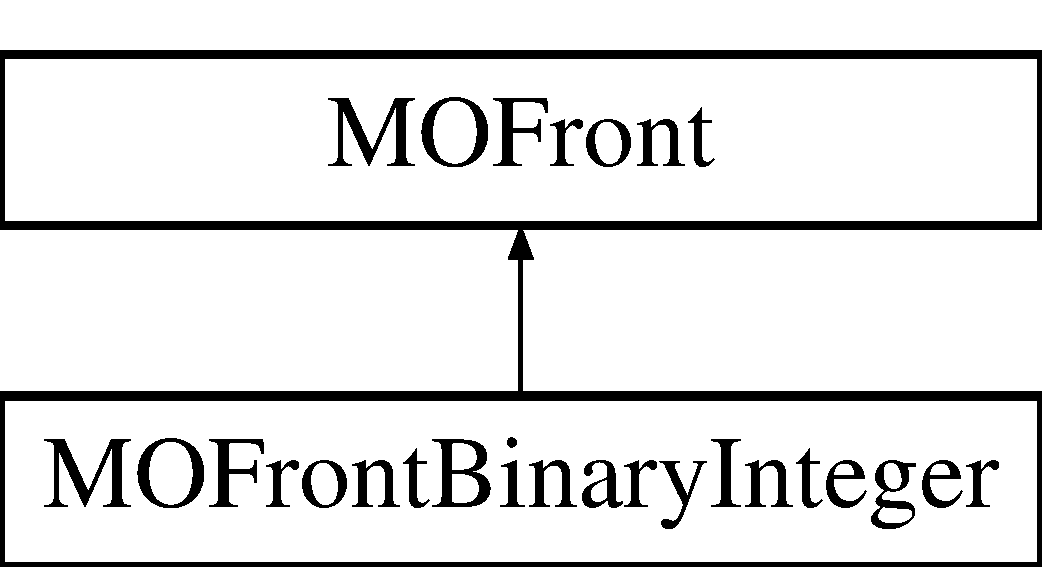
\includegraphics[height=2.000000cm]{da/dbd/classMOFrontBinaryInteger}
\end{center}
\end{figure}
\subsection*{Public Member Functions}
\begin{DoxyCompactItemize}
\item 
\mbox{\Hypertarget{classMOFrontBinaryInteger_a5236a5002cc410e8dec597c12256f6b0}\label{classMOFrontBinaryInteger_a5236a5002cc410e8dec597c12256f6b0}} 
{\bfseries M\+O\+Front\+Binary\+Integer} (const \mbox{\hyperlink{classIndividual}{Individual}} $\ast$ej\+Ind, bool copy\+On\+Insert, bool delete\+On\+Destroy)
\item 
\mbox{\Hypertarget{classMOFrontBinaryInteger_a3c38e6b6e8beb50b43a46863afdf2234}\label{classMOFrontBinaryInteger_a3c38e6b6e8beb50b43a46863afdf2234}} 
unsigned int {\bfseries get\+Front\+Size} (void)
\item 
\mbox{\Hypertarget{classMOFrontBinaryInteger_aff530861f58e5073109fc63822fc68ba}\label{classMOFrontBinaryInteger_aff530861f58e5073109fc63822fc68ba}} 
\mbox{\hyperlink{classIndividual}{Individual}} $\ast$ {\bfseries get\+Ind} (int index\+Ind) const
\item 
\mbox{\Hypertarget{classMOFrontBinaryInteger_a3aebfdcab8b576f41e8ae9b03fdec4f2}\label{classMOFrontBinaryInteger_a3aebfdcab8b576f41e8ae9b03fdec4f2}} 
void {\bfseries get\+All\+Individuals} (vector$<$ \mbox{\hyperlink{classIndividual}{Individual}} $\ast$$>$ \&front)
\item 
\mbox{\Hypertarget{classMOFrontBinaryInteger_a89e37b3811333af72d1ade0e3e9a429a}\label{classMOFrontBinaryInteger_a89e37b3811333af72d1ade0e3e9a429a}} 
void {\bfseries get\+Inds} (int n\+Ind, vector$<$ \mbox{\hyperlink{classIndividual}{Individual}} $\ast$$>$ \&inds)
\item 
\mbox{\Hypertarget{classMOFrontBinaryInteger_a09556773bf768ab014ad4fc66a9a5ebe}\label{classMOFrontBinaryInteger_a09556773bf768ab014ad4fc66a9a5ebe}} 
bool {\bfseries insert} (\mbox{\hyperlink{classIndividual}{Individual}} $\ast$ind, int \&erased, bool \&iguales)
\item 
\mbox{\Hypertarget{classMOFrontBinaryInteger_a0c27eeaf5d77b5a934283cd9b42db990}\label{classMOFrontBinaryInteger_a0c27eeaf5d77b5a934283cd9b42db990}} 
void {\bfseries clear} ()
\item 
\mbox{\Hypertarget{classMOFrontBinaryInteger_ad0a4e91b4ce764989e4cff751a1cebc0}\label{classMOFrontBinaryInteger_ad0a4e91b4ce764989e4cff751a1cebc0}} 
void {\bfseries send} (int dest)
\item 
\mbox{\Hypertarget{classMOFrontBinaryInteger_ad154fc956fd7763c22e2d6240e98ace0}\label{classMOFrontBinaryInteger_ad154fc956fd7763c22e2d6240e98ace0}} 
void {\bfseries crow\+Order} (const unsigned int final\+Size)
\end{DoxyCompactItemize}
\subsection*{Static Public Attributes}
\begin{DoxyCompactItemize}
\item 
\mbox{\Hypertarget{classMOFrontBinaryInteger_a504cbd16e49176bfb1da068724e1855d}\label{classMOFrontBinaryInteger_a504cbd16e49176bfb1da068724e1855d}} 
static int {\bfseries obj\+Order}
\end{DoxyCompactItemize}
\subsection*{Private Attributes}
\begin{DoxyCompactItemize}
\item 
\mbox{\Hypertarget{classMOFrontBinaryInteger_abd62291c97b834b9b638cf07b90ef16e}\label{classMOFrontBinaryInteger_abd62291c97b834b9b638cf07b90ef16e}} 
vector$<$ \mbox{\hyperlink{classIndividual}{Individual}} $\ast$ $>$ {\bfseries front}
\item 
\mbox{\Hypertarget{classMOFrontBinaryInteger_a202f9e78cedee3e6f23b9eb9fdaebd99}\label{classMOFrontBinaryInteger_a202f9e78cedee3e6f23b9eb9fdaebd99}} 
int {\bfseries obj\+Index}
\item 
\mbox{\Hypertarget{classMOFrontBinaryInteger_a05e0ccf73f5591c6886bbb878e13e496}\label{classMOFrontBinaryInteger_a05e0ccf73f5591c6886bbb878e13e496}} 
int {\bfseries obj\+Non\+Index}
\item 
\mbox{\Hypertarget{classMOFrontBinaryInteger_a55bc21f3a3c4814bd2420dd2dca15104}\label{classMOFrontBinaryInteger_a55bc21f3a3c4814bd2420dd2dca15104}} 
int {\bfseries min\+Obj\+Index}
\item 
\mbox{\Hypertarget{classMOFrontBinaryInteger_a742df4647e879e87a29165a1d7ea401b}\label{classMOFrontBinaryInteger_a742df4647e879e87a29165a1d7ea401b}} 
int {\bfseries max\+Obj\+Index}
\end{DoxyCompactItemize}
\subsection*{Additional Inherited Members}


The documentation for this class was generated from the following files\+:\begin{DoxyCompactItemize}
\item 
M\+O\+Front\+Binary\+Integer.\+h\item 
M\+O\+Front\+Binary\+Integer.\+cpp\end{DoxyCompactItemize}

\hypertarget{classMOFrontVector}{}\section{M\+O\+Front\+Vector Class Reference}
\label{classMOFrontVector}\index{M\+O\+Front\+Vector@{M\+O\+Front\+Vector}}
Inheritance diagram for M\+O\+Front\+Vector\+:\begin{figure}[H]
\begin{center}
\leavevmode
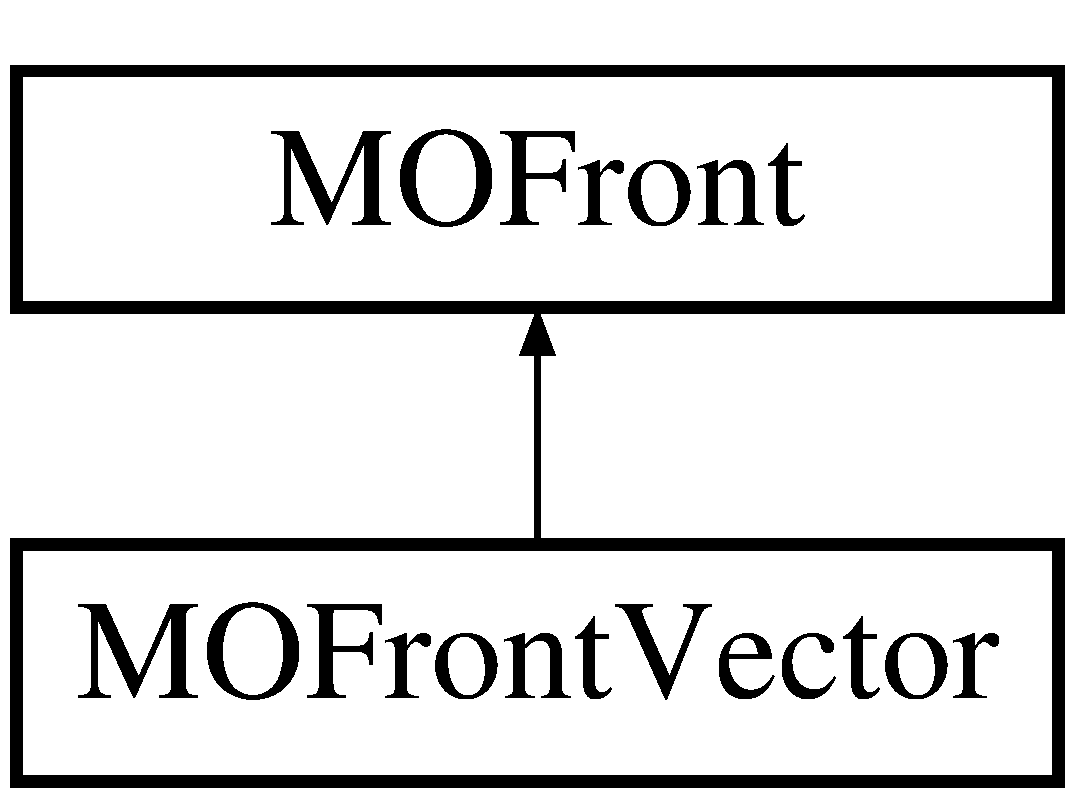
\includegraphics[height=2.000000cm]{d3/d9e/classMOFrontVector}
\end{center}
\end{figure}
\subsection*{Public Member Functions}
\begin{DoxyCompactItemize}
\item 
\mbox{\Hypertarget{classMOFrontVector_a8aa874eec535a01396476660d26d1d92}\label{classMOFrontVector_a8aa874eec535a01396476660d26d1d92}} 
{\bfseries M\+O\+Front\+Vector} (const \mbox{\hyperlink{classIndividual}{Individual}} $\ast$ej\+Ind, bool copy\+On\+Insert, bool delete\+On\+Destroy)
\item 
\mbox{\Hypertarget{classMOFrontVector_a097ff296747469de470d1bbe8ffea8d0}\label{classMOFrontVector_a097ff296747469de470d1bbe8ffea8d0}} 
unsigned int {\bfseries get\+Front\+Size} (void)
\item 
\mbox{\Hypertarget{classMOFrontVector_ab3010c5013a5c70bae8d63d28afac7ef}\label{classMOFrontVector_ab3010c5013a5c70bae8d63d28afac7ef}} 
\mbox{\hyperlink{classIndividual}{Individual}} $\ast$ {\bfseries get\+Ind} (int index\+Ind) const
\item 
\mbox{\Hypertarget{classMOFrontVector_aeb03f858624e260b8cf9e6b258cea16a}\label{classMOFrontVector_aeb03f858624e260b8cf9e6b258cea16a}} 
void {\bfseries get\+All\+Individuals} (vector$<$ \mbox{\hyperlink{classIndividual}{Individual}} $\ast$$>$ \&f)
\item 
\mbox{\Hypertarget{classMOFrontVector_afa7bbc5c138b98af007f606973ad44f8}\label{classMOFrontVector_afa7bbc5c138b98af007f606973ad44f8}} 
void {\bfseries get\+Inds} (int n\+Ind, vector$<$ \mbox{\hyperlink{classIndividual}{Individual}} $\ast$$>$ \&inds)
\item 
\mbox{\Hypertarget{classMOFrontVector_af1f3b371e34b724f717e925e8eff9895}\label{classMOFrontVector_af1f3b371e34b724f717e925e8eff9895}} 
bool {\bfseries insert} (\mbox{\hyperlink{classIndividual}{Individual}} $\ast$ind, int \&erased, bool \&iguales)
\item 
\mbox{\Hypertarget{classMOFrontVector_af953106f10ca1ea2cf4ae9f57071fba8}\label{classMOFrontVector_af953106f10ca1ea2cf4ae9f57071fba8}} 
void {\bfseries clear} ()
\item 
\mbox{\Hypertarget{classMOFrontVector_a38858522f170894c482bcd3abc57d6b4}\label{classMOFrontVector_a38858522f170894c482bcd3abc57d6b4}} 
void {\bfseries send} (int dest)
\item 
\mbox{\Hypertarget{classMOFrontVector_a1b62fed1b181930e5ce6ce4b6e792f21}\label{classMOFrontVector_a1b62fed1b181930e5ce6ce4b6e792f21}} 
void {\bfseries crow\+Order} (const unsigned int final\+Size)
\end{DoxyCompactItemize}
\subsection*{Static Public Attributes}
\begin{DoxyCompactItemize}
\item 
\mbox{\Hypertarget{classMOFrontVector_a40e2da74155fdb19404fa24a381e0aef}\label{classMOFrontVector_a40e2da74155fdb19404fa24a381e0aef}} 
static int {\bfseries obj\+Order}
\end{DoxyCompactItemize}
\subsection*{Private Attributes}
\begin{DoxyCompactItemize}
\item 
\mbox{\Hypertarget{classMOFrontVector_aab766723ee771daa01a129fe4e489287}\label{classMOFrontVector_aab766723ee771daa01a129fe4e489287}} 
vector$<$ \mbox{\hyperlink{classIndividual}{Individual}} $\ast$ $>$ {\bfseries front}
\end{DoxyCompactItemize}
\subsection*{Additional Inherited Members}


The documentation for this class was generated from the following files\+:\begin{DoxyCompactItemize}
\item 
M\+O\+Front\+Vector.\+h\item 
M\+O\+Front\+Vector.\+cpp\end{DoxyCompactItemize}

\hypertarget{classMultiObjectivization}{}\section{Multi\+Objectivization Class Reference}
\label{classMultiObjectivization}\index{Multi\+Objectivization@{Multi\+Objectivization}}
Inheritance diagram for Multi\+Objectivization\+:\begin{figure}[H]
\begin{center}
\leavevmode
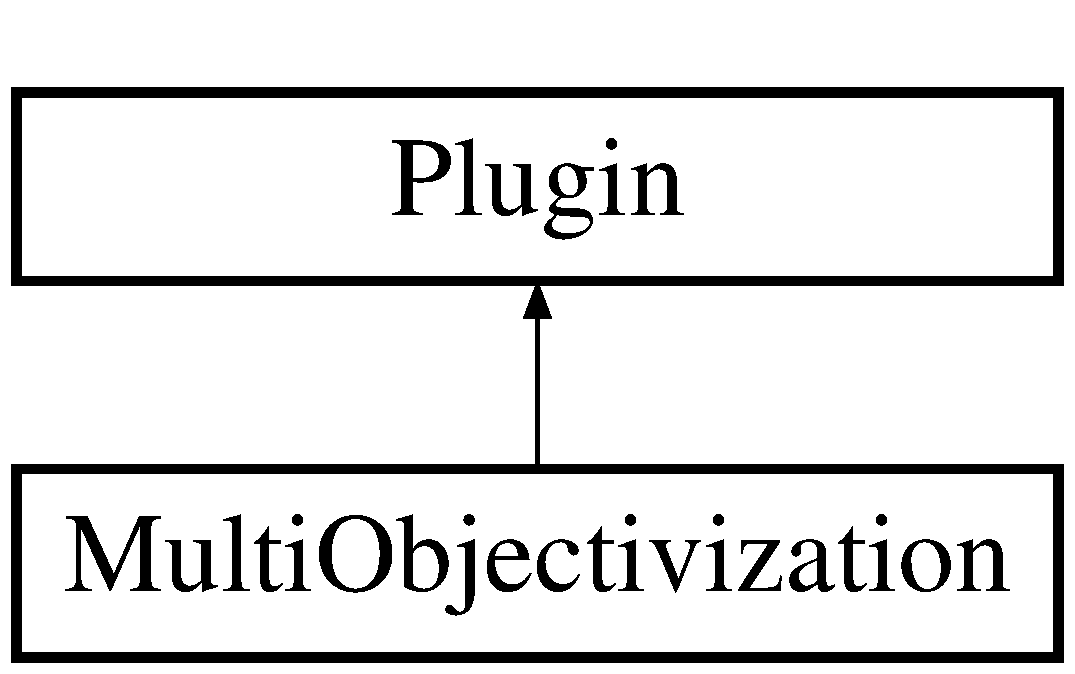
\includegraphics[height=2.000000cm]{d8/db8/classMultiObjectivization}
\end{center}
\end{figure}
\subsection*{Public Member Functions}
\begin{DoxyCompactItemize}
\item 
\mbox{\Hypertarget{classMultiObjectivization_a080d1d8aed13ed15918ec506779c03cd}\label{classMultiObjectivization_a080d1d8aed13ed15918ec506779c03cd}} 
virtual void {\bfseries convert\+To\+Multi\+Objective} (vector$<$ \mbox{\hyperlink{classIndividual}{Individual}} $\ast$$>$ $\ast$parents, vector$<$ \mbox{\hyperlink{classIndividual}{Individual}} $\ast$$>$ $\ast$off\+Springs, vector$<$ \mbox{\hyperlink{classIndividual}{Individual}} $\ast$$>$ $\ast$reference, int ord\+Obj, int num\+Generation)=0
\item 
\mbox{\Hypertarget{classMultiObjectivization_a95936caf2862903ac3e4026382afe7dd}\label{classMultiObjectivization_a95936caf2862903ac3e4026382afe7dd}} 
virtual int {\bfseries get\+Opt\+Direction} ()=0
\item 
\mbox{\Hypertarget{classMultiObjectivization_afbd6118fbc372dd5f2a0a9f138e42af5}\label{classMultiObjectivization_afbd6118fbc372dd5f2a0a9f138e42af5}} 
virtual void {\bfseries initiallization} (\mbox{\hyperlink{classIndividual}{Individual}} $\ast$ej\+Ind)
\end{DoxyCompactItemize}
\subsection*{Additional Inherited Members}


The documentation for this class was generated from the following file\+:\begin{DoxyCompactItemize}
\item 
Multi\+Objectivization.\+h\end{DoxyCompactItemize}

\hypertarget{classMutation}{}\section{Mutation Class Reference}
\label{classMutation}\index{Mutation@{Mutation}}
Inheritance diagram for Mutation\+:\begin{figure}[H]
\begin{center}
\leavevmode
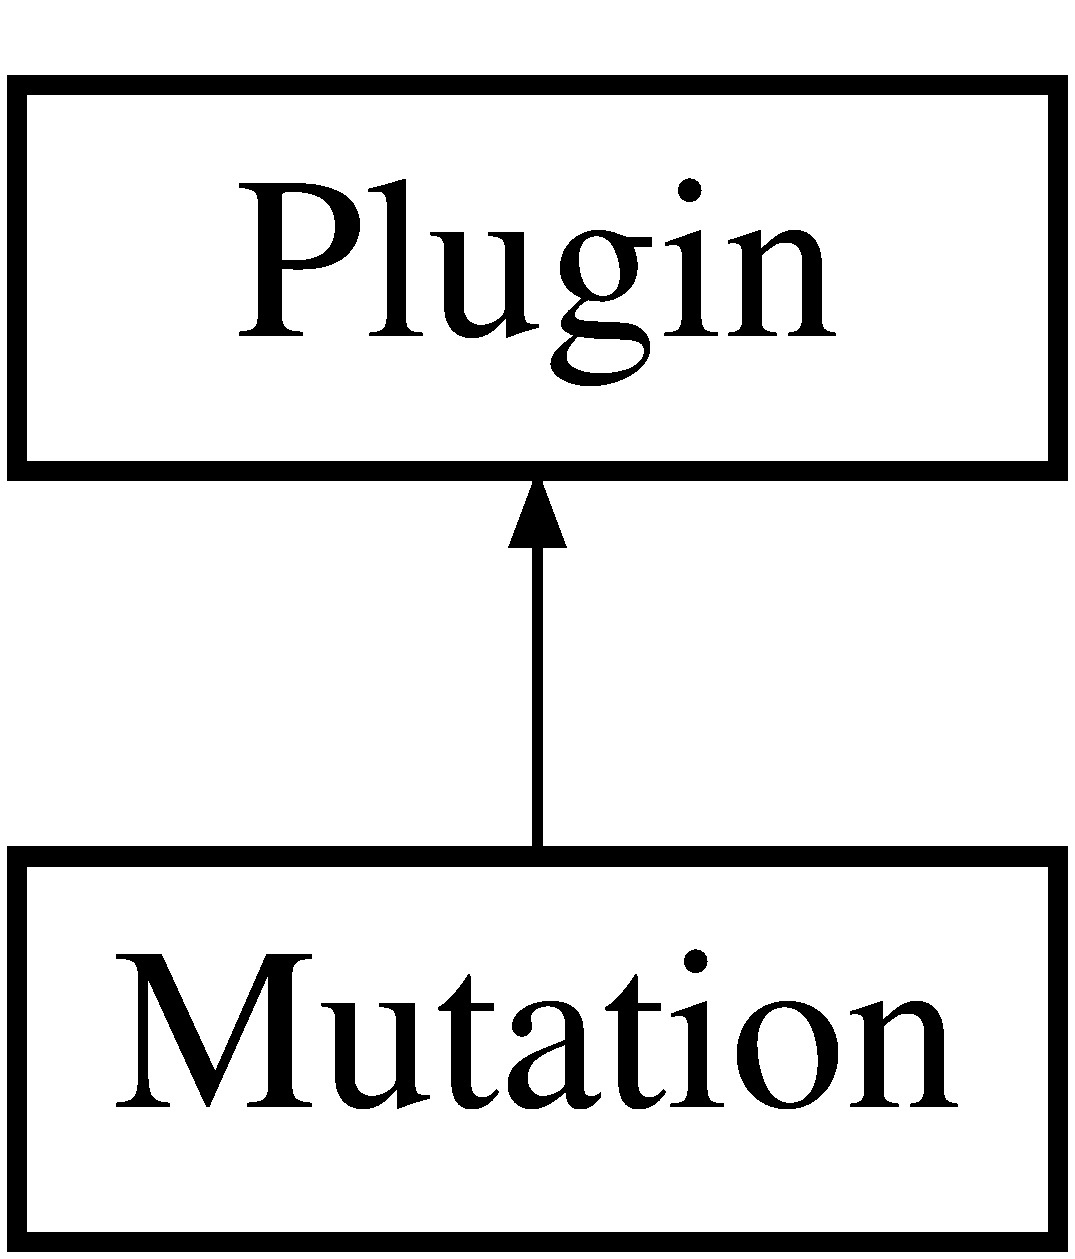
\includegraphics[height=2.000000cm]{d9/df6/classMutation}
\end{center}
\end{figure}
\subsection*{Public Member Functions}
\begin{DoxyCompactItemize}
\item 
\mbox{\Hypertarget{classMutation_a9a61940dc548404c7e6aa7a94ed8808a}\label{classMutation_a9a61940dc548404c7e6aa7a94ed8808a}} 
virtual void {\bfseries mutation} (\mbox{\hyperlink{classIndividual}{Individual}} $\ast$ind, const double pm)=0
\end{DoxyCompactItemize}
\subsection*{Additional Inherited Members}


The documentation for this class was generated from the following file\+:\begin{DoxyCompactItemize}
\item 
Mutation.\+h\end{DoxyCompactItemize}

\hypertarget{classOutputPrinter}{}\section{Output\+Printer Class Reference}
\label{classOutputPrinter}\index{Output\+Printer@{Output\+Printer}}
Inheritance diagram for Output\+Printer\+:\begin{figure}[H]
\begin{center}
\leavevmode
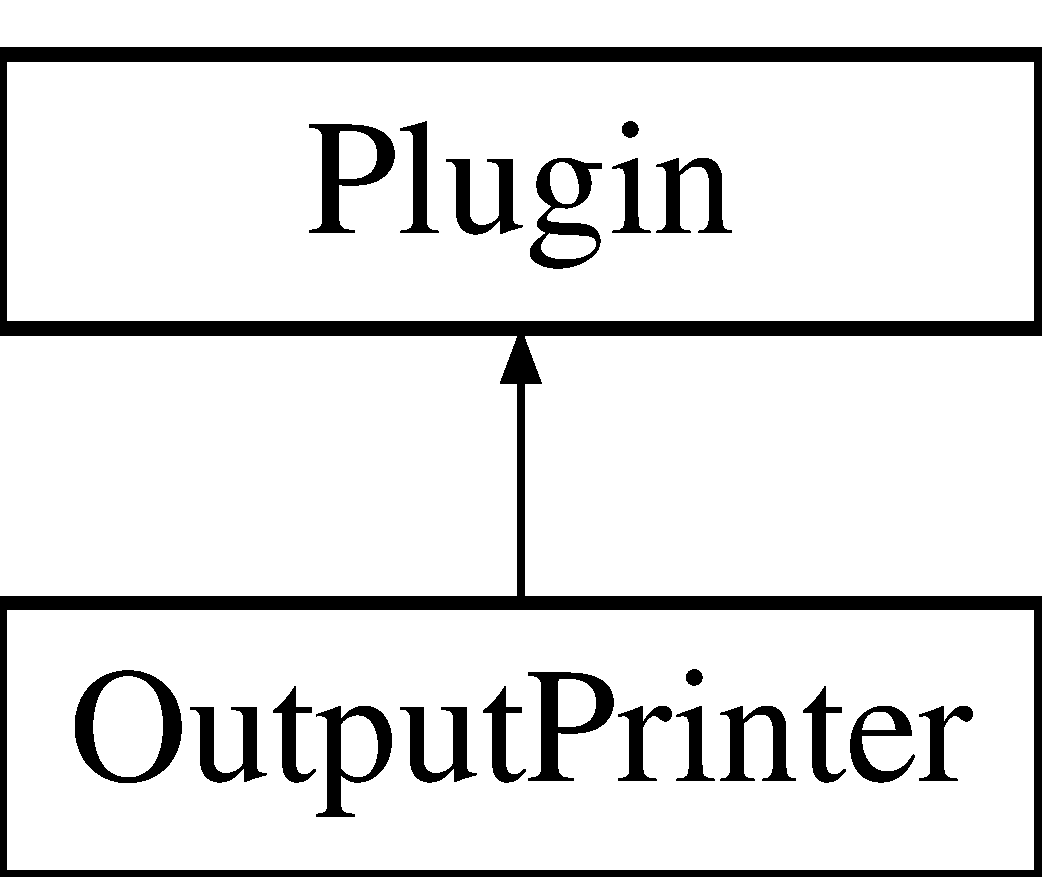
\includegraphics[height=2.000000cm]{dd/d6f/classOutputPrinter}
\end{center}
\end{figure}
\subsection*{Public Member Functions}
\begin{DoxyCompactItemize}
\item 
\mbox{\Hypertarget{classOutputPrinter_ae7e777123d103ccd0e8ad77a511aaaab}\label{classOutputPrinter_ae7e777123d103ccd0e8ad77a511aaaab}} 
virtual void {\bfseries print\+Solution} (\mbox{\hyperlink{classEA}{EA}} $\ast$ga, bool end)=0
\item 
\mbox{\Hypertarget{classOutputPrinter_a86e3c9a97a5ad0eb71c8701f7c8a622f}\label{classOutputPrinter_a86e3c9a97a5ad0eb71c8701f7c8a622f}} 
virtual void {\bfseries print\+Init} (\mbox{\hyperlink{classEA}{EA}} $\ast$ga)=0
\item 
\mbox{\Hypertarget{classOutputPrinter_a6902ce594bdec28859a84afb4f448112}\label{classOutputPrinter_a6902ce594bdec28859a84afb4f448112}} 
virtual void {\bfseries finish} ()=0
\end{DoxyCompactItemize}
\subsection*{Additional Inherited Members}


The documentation for this class was generated from the following file\+:\begin{DoxyCompactItemize}
\item 
Output\+Printer.\+h\end{DoxyCompactItemize}

\hypertarget{classPlugin}{}\section{Plugin Class Reference}
\label{classPlugin}\index{Plugin@{Plugin}}
Inheritance diagram for Plugin\+:\begin{figure}[H]
\begin{center}
\leavevmode
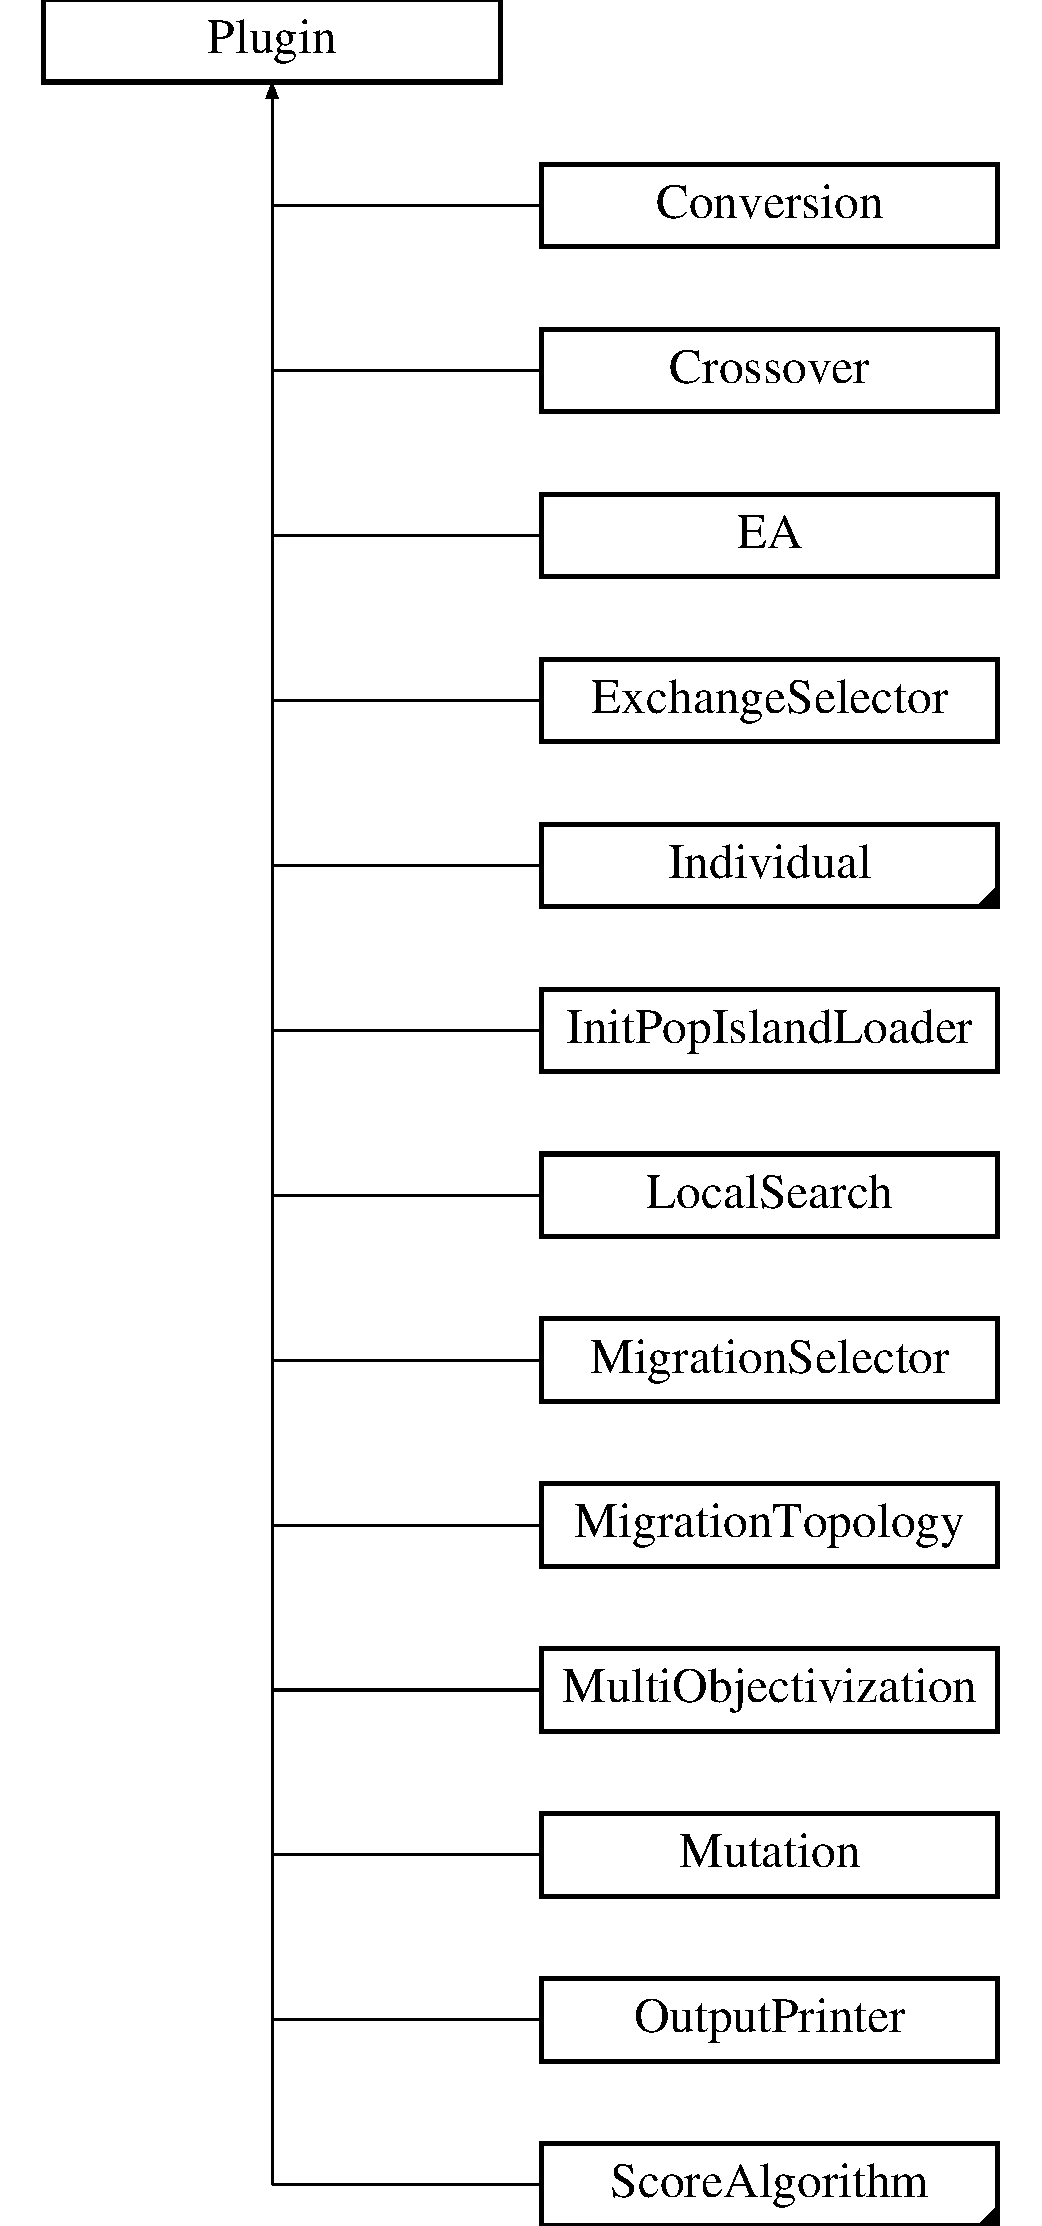
\includegraphics[height=12.000000cm]{db/df9/classPlugin}
\end{center}
\end{figure}
\subsection*{Public Member Functions}
\begin{DoxyCompactItemize}
\item 
\mbox{\Hypertarget{classPlugin_aef4aa350c3420324604b368702a48a4c}\label{classPlugin_aef4aa350c3420324604b368702a48a4c}} 
virtual bool {\bfseries init} (const vector$<$ string $>$ \&params)
\item 
\mbox{\Hypertarget{classPlugin_ac86ec12b0b9e91653fa52c8056cf4f52}\label{classPlugin_ac86ec12b0b9e91653fa52c8056cf4f52}} 
virtual string {\bfseries get\+Name} () const
\item 
\mbox{\Hypertarget{classPlugin_a998ff760a6a53a08621ee01c051c5c0a}\label{classPlugin_a998ff760a6a53a08621ee01c051c5c0a}} 
virtual void {\bfseries set\+Name} (const string \&n)
\item 
\mbox{\Hypertarget{classPlugin_aa52917db69bb89c02ce64fc5d2b16c5c}\label{classPlugin_aa52917db69bb89c02ce64fc5d2b16c5c}} 
virtual string {\bfseries get\+Parameter\+Name} (int i) const
\item 
\mbox{\Hypertarget{classPlugin_a8ec9c87432a1e4040fdc013ad269db17}\label{classPlugin_a8ec9c87432a1e4040fdc013ad269db17}} 
virtual string {\bfseries get\+Parameter\+Value} (int i) const
\item 
\mbox{\Hypertarget{classPlugin_a73cc5d43de734e4fa8bd320f52dd8528}\label{classPlugin_a73cc5d43de734e4fa8bd320f52dd8528}} 
virtual int {\bfseries get\+Number\+Of\+Parameters} () const
\end{DoxyCompactItemize}
\subsection*{Public Attributes}
\begin{DoxyCompactItemize}
\item 
\mbox{\Hypertarget{classPlugin_ab562544338cd35effdff475f1d019bb2}\label{classPlugin_ab562544338cd35effdff475f1d019bb2}} 
string {\bfseries name}
\end{DoxyCompactItemize}


The documentation for this class was generated from the following files\+:\begin{DoxyCompactItemize}
\item 
Plugin.\+h\item 
Plugin.\+cpp\end{DoxyCompactItemize}

\hypertarget{classScoreAlgorithm}{}\section{Score\+Algorithm Class Reference}
\label{classScoreAlgorithm}\index{Score\+Algorithm@{Score\+Algorithm}}
Inheritance diagram for Score\+Algorithm\+:\begin{figure}[H]
\begin{center}
\leavevmode
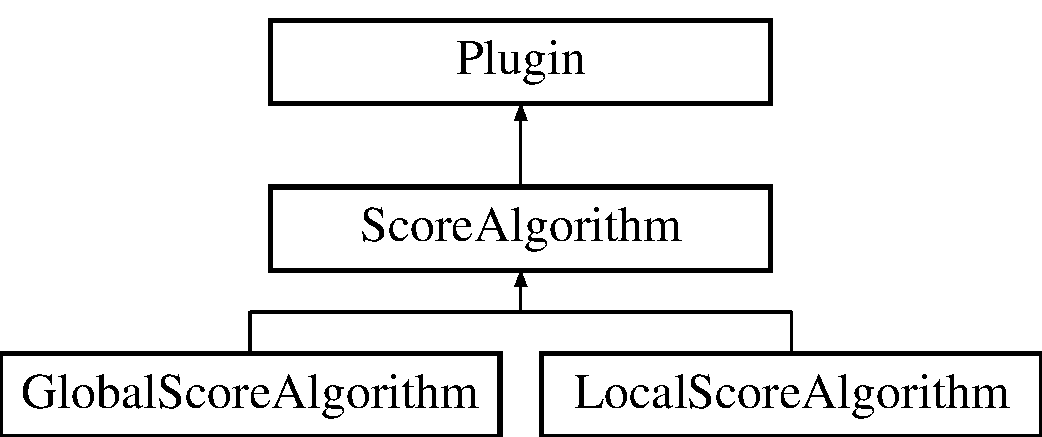
\includegraphics[height=3.000000cm]{da/de1/classScoreAlgorithm}
\end{center}
\end{figure}
\subsection*{Public Member Functions}
\begin{DoxyCompactItemize}
\item 
\mbox{\Hypertarget{classScoreAlgorithm_aca316a7c8fb4a7d65793142ffb0854c0}\label{classScoreAlgorithm_aca316a7c8fb4a7d65793142ffb0854c0}} 
{\bfseries Score\+Algorithm} (const int type)
\item 
\mbox{\Hypertarget{classScoreAlgorithm_aa5a21e0bd7246db2f4bf4994f63badbe}\label{classScoreAlgorithm_aa5a21e0bd7246db2f4bf4994f63badbe}} 
int {\bfseries get\+Type} () const
\item 
\mbox{\Hypertarget{classScoreAlgorithm_ac8cc1949e42bc5e7f9b40a2fd5431fce}\label{classScoreAlgorithm_ac8cc1949e42bc5e7f9b40a2fd5431fce}} 
virtual bool {\bfseries init} (const vector$<$ string $>$ \&params)
\item 
\mbox{\Hypertarget{classScoreAlgorithm_adebfd2133cc2531c4573eb4447285dcc}\label{classScoreAlgorithm_adebfd2133cc2531c4573eb4447285dcc}} 
virtual void {\bfseries begins} (const int alg\+Id, const int conf\+Id, const int island\+Id)
\item 
\mbox{\Hypertarget{classScoreAlgorithm_a68a608ca6d436baa5ac73b39b29215dc}\label{classScoreAlgorithm_a68a608ca6d436baa5ac73b39b29215dc}} 
virtual void {\bfseries ends} (const int alg\+Id, const int conf\+Id, const int island\+Id)
\item 
\mbox{\Hypertarget{classScoreAlgorithm_a0366ab9698f481f382d676d77feebf7b}\label{classScoreAlgorithm_a0366ab9698f481f382d676d77feebf7b}} 
void {\bfseries set\+Configurations} (const vector$<$ int $>$ \&configs)
\item 
\mbox{\Hypertarget{classScoreAlgorithm_a88bb035f0b88fa201add6766fec426b5}\label{classScoreAlgorithm_a88bb035f0b88fa201add6766fec426b5}} 
virtual int {\bfseries get\+Direction} () const =0
\end{DoxyCompactItemize}
\subsection*{Protected Member Functions}
\begin{DoxyCompactItemize}
\item 
\mbox{\Hypertarget{classScoreAlgorithm_a96a7912c56aae7c5eeba05e9c7d73f19}\label{classScoreAlgorithm_a96a7912c56aae7c5eeba05e9c7d73f19}} 
int {\bfseries get\+Number\+Of\+Algorithms} ()
\item 
\mbox{\Hypertarget{classScoreAlgorithm_ac67021a4b1390d39649988c1512df779}\label{classScoreAlgorithm_ac67021a4b1390d39649988c1512df779}} 
int {\bfseries get\+Number\+Of\+Configurations} (int alg\+Id)
\item 
\mbox{\Hypertarget{classScoreAlgorithm_aed17e61b133b57a1d10202eebd3fc06f}\label{classScoreAlgorithm_aed17e61b133b57a1d10202eebd3fc06f}} 
int {\bfseries get\+Number\+Of\+Configurations} ()
\end{DoxyCompactItemize}
\subsection*{Private Attributes}
\begin{DoxyCompactItemize}
\item 
\mbox{\Hypertarget{classScoreAlgorithm_a5db73d908a5fcc2c6c28914f6ba3532b}\label{classScoreAlgorithm_a5db73d908a5fcc2c6c28914f6ba3532b}} 
int {\bfseries number\+Of\+Configurations}
\item 
\mbox{\Hypertarget{classScoreAlgorithm_a194ba64e3bef5f5e4d9eed35c896a9a3}\label{classScoreAlgorithm_a194ba64e3bef5f5e4d9eed35c896a9a3}} 
int {\bfseries type}
\item 
\mbox{\Hypertarget{classScoreAlgorithm_a4683849279cb7a803919f09c2d13f907}\label{classScoreAlgorithm_a4683849279cb7a803919f09c2d13f907}} 
vector$<$ int $>$ {\bfseries configs}
\end{DoxyCompactItemize}
\subsection*{Additional Inherited Members}


The documentation for this class was generated from the following files\+:\begin{DoxyCompactItemize}
\item 
Score\+Algorithm.\+h\item 
Score\+Algorithm.\+cpp\end{DoxyCompactItemize}

\hypertarget{classSimpleIndividual}{}\section{Simple\+Individual Class Reference}
\label{classSimpleIndividual}\index{Simple\+Individual@{Simple\+Individual}}
Inheritance diagram for Simple\+Individual\+:\begin{figure}[H]
\begin{center}
\leavevmode
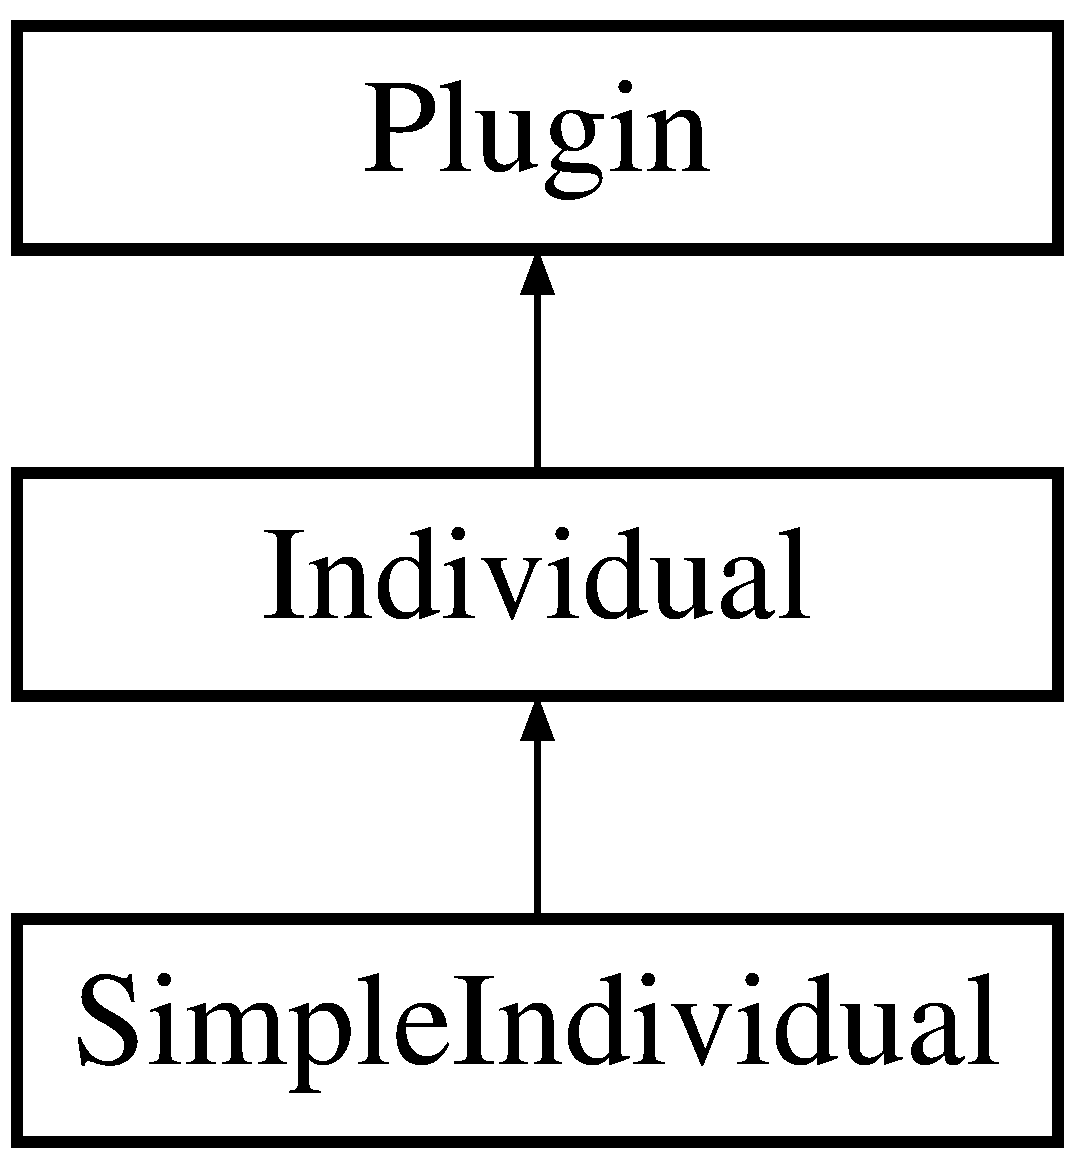
\includegraphics[height=3.000000cm]{d3/da8/classSimpleIndividual}
\end{center}
\end{figure}
\subsection*{Public Member Functions}
\begin{DoxyCompactItemize}
\item 
\mbox{\Hypertarget{classSimpleIndividual_a120e65e839faa693d8ad12d08c8b476a}\label{classSimpleIndividual_a120e65e839faa693d8ad12d08c8b476a}} 
{\bfseries Simple\+Individual} (int n\+Var, int n\+Obj)
\item 
\mbox{\Hypertarget{classSimpleIndividual_aad10ed7c1037417d8a1c48ad794d4068}\label{classSimpleIndividual_aad10ed7c1037417d8a1c48ad794d4068}} 
void {\bfseries evaluate} (void)
\item 
\mbox{\Hypertarget{classSimpleIndividual_ac28c4bb3a587763fc0b6264cb3c87479}\label{classSimpleIndividual_ac28c4bb3a587763fc0b6264cb3c87479}} 
double {\bfseries get\+Maximum} (const int i) const
\item 
\mbox{\Hypertarget{classSimpleIndividual_ae35587cc860f4281ed4f2f0e196a58f4}\label{classSimpleIndividual_ae35587cc860f4281ed4f2f0e196a58f4}} 
double {\bfseries get\+Minimum} (const int i) const
\item 
\mbox{\Hypertarget{classSimpleIndividual_ab7b07fd70f90fa024179ed05b26ea2f7}\label{classSimpleIndividual_ab7b07fd70f90fa024179ed05b26ea2f7}} 
unsigned int {\bfseries get\+Opt\+Direction} (const int i) const
\item 
\mbox{\Hypertarget{classSimpleIndividual_af6d469ce795e3862d62b90d97b32d50a}\label{classSimpleIndividual_af6d469ce795e3862d62b90d97b32d50a}} 
void {\bfseries set\+Opt\+Direction} (const int i, const int d)
\item 
\mbox{\Hypertarget{classSimpleIndividual_ab13d92d0525fa23289fe99fc25954e12}\label{classSimpleIndividual_ab13d92d0525fa23289fe99fc25954e12}} 
\mbox{\hyperlink{classIndividual}{Individual}} $\ast$ {\bfseries clone} (void) const
\end{DoxyCompactItemize}
\subsection*{Private Attributes}
\begin{DoxyCompactItemize}
\item 
\mbox{\Hypertarget{classSimpleIndividual_a0c4b0d0759b905e1b66c2ab0588e32ef}\label{classSimpleIndividual_a0c4b0d0759b905e1b66c2ab0588e32ef}} 
vector$<$ double $>$ {\bfseries opt\+Directions}
\end{DoxyCompactItemize}
\subsection*{Additional Inherited Members}


The documentation for this class was generated from the following files\+:\begin{DoxyCompactItemize}
\item 
Simple\+Individual.\+h\item 
Simple\+Individual.\+cpp\end{DoxyCompactItemize}

\hypertarget{structTAlgorithm}{}\section{T\+Algorithm Struct Reference}
\label{structTAlgorithm}\index{T\+Algorithm@{T\+Algorithm}}
\subsection*{Public Attributes}
\begin{DoxyCompactItemize}
\item 
\mbox{\Hypertarget{structTAlgorithm_a5e7db46febcdf28a01d5e2e32547b976}\label{structTAlgorithm_a5e7db46febcdf28a01d5e2e32547b976}} 
int {\bfseries crit\+Stop}
\item 
\mbox{\Hypertarget{structTAlgorithm_a80ca0307e9bf6d720214af1246baf9d4}\label{structTAlgorithm_a80ca0307e9bf6d720214af1246baf9d4}} 
double {\bfseries value\+SC}
\item 
\mbox{\Hypertarget{structTAlgorithm_ab99e2fb15d3a6249af2f526283a5cd66}\label{structTAlgorithm_ab99e2fb15d3a6249af2f526283a5cd66}} 
string {\bfseries individual\+Name}
\item 
\mbox{\Hypertarget{structTAlgorithm_a3d5c273a9c7a83a211ca321834c4fc71}\label{structTAlgorithm_a3d5c273a9c7a83a211ca321834c4fc71}} 
string {\bfseries individual\+Params}
\item 
\mbox{\Hypertarget{structTAlgorithm_a56ceda030117e9fa883436fd3800fd0c}\label{structTAlgorithm_a56ceda030117e9fa883436fd3800fd0c}} 
string {\bfseries migration\+Selector\+Name}
\item 
\mbox{\Hypertarget{structTAlgorithm_aed07e57052ddc6db16afc20473d2f9a2}\label{structTAlgorithm_aed07e57052ddc6db16afc20473d2f9a2}} 
string {\bfseries exchange\+Selector\+Name}
\item 
\mbox{\Hypertarget{structTAlgorithm_a8782ffcecaaa1bde0b1e564b157ea2fe}\label{structTAlgorithm_a8782ffcecaaa1bde0b1e564b157ea2fe}} 
string {\bfseries mutation\+Name}
\item 
\mbox{\Hypertarget{structTAlgorithm_afdefbc9ce4b18ef6d403946cc3049d71}\label{structTAlgorithm_afdefbc9ce4b18ef6d403946cc3049d71}} 
string {\bfseries crossover\+Name}
\item 
\mbox{\Hypertarget{structTAlgorithm_a4ea8eea24e6f3e234ab1ead97068664f}\label{structTAlgorithm_a4ea8eea24e6f3e234ab1ead97068664f}} 
string {\bfseries local\+Search\+Name}
\item 
\mbox{\Hypertarget{structTAlgorithm_abe21dce696d82a955ae0afd359a00fe4}\label{structTAlgorithm_abe21dce696d82a955ae0afd359a00fe4}} 
string {\bfseries multi\+Objectivization\+Name}
\item 
\mbox{\Hypertarget{structTAlgorithm_ae66c69b9f125acb363a8662abd15a709}\label{structTAlgorithm_ae66c69b9f125acb363a8662abd15a709}} 
\mbox{\hyperlink{classMigrationSelector}{Migration\+Selector}} $\ast$ {\bfseries migration\+Selector}
\item 
\mbox{\Hypertarget{structTAlgorithm_a4fac798faf055d9d78771e541c46a98a}\label{structTAlgorithm_a4fac798faf055d9d78771e541c46a98a}} 
\mbox{\hyperlink{classExchangeSelector}{Exchange\+Selector}} $\ast$ {\bfseries exchange\+Selector}
\item 
\mbox{\Hypertarget{structTAlgorithm_af30d430da8ec08152c4a5056b29eaed2}\label{structTAlgorithm_af30d430da8ec08152c4a5056b29eaed2}} 
\mbox{\hyperlink{classMutation}{Mutation}} $\ast$ {\bfseries mutation}
\item 
\mbox{\Hypertarget{structTAlgorithm_a3f859a16df8b05dd210e89e2212285d1}\label{structTAlgorithm_a3f859a16df8b05dd210e89e2212285d1}} 
\mbox{\hyperlink{classCrossover}{Crossover}} $\ast$ {\bfseries crossover}
\item 
\mbox{\Hypertarget{structTAlgorithm_aa3ceb63aec5a19d377c73f777ae23e47}\label{structTAlgorithm_aa3ceb63aec5a19d377c73f777ae23e47}} 
\mbox{\hyperlink{classLocalSearch}{Local\+Search}} $\ast$ {\bfseries local\+Search}
\item 
\mbox{\Hypertarget{structTAlgorithm_ae61847fa5f79552ee797adf1386c5b4f}\label{structTAlgorithm_ae61847fa5f79552ee797adf1386c5b4f}} 
vector$<$ string $>$ {\bfseries local\+Search\+Params}
\item 
\mbox{\Hypertarget{structTAlgorithm_a08323c63e8b184fa41165f962e82de6a}\label{structTAlgorithm_a08323c63e8b184fa41165f962e82de6a}} 
\mbox{\hyperlink{classMultiObjectivization}{Multi\+Objectivization}} $\ast$ {\bfseries multi\+Objectivization}
\item 
\mbox{\Hypertarget{structTAlgorithm_a7f115a397ed8203dde37de6cc9c86777}\label{structTAlgorithm_a7f115a397ed8203dde37de6cc9c86777}} 
vector$<$ string $>$ {\bfseries multi\+Objectivization\+Params}
\item 
\mbox{\Hypertarget{structTAlgorithm_a8a80833813e0e39a616ba16cb5165c14}\label{structTAlgorithm_a8a80833813e0e39a616ba16cb5165c14}} 
int {\bfseries solution\+Source}
\item 
\mbox{\Hypertarget{structTAlgorithm_a7e65f546da96d6fe3d670cb508e8b540}\label{structTAlgorithm_a7e65f546da96d6fe3d670cb508e8b540}} 
\mbox{\hyperlink{classIndividual}{Individual}} $\ast$ {\bfseries ind}
\item 
\mbox{\Hypertarget{structTAlgorithm_a09f6e37f7bb6931e00854e4a5c91ce18}\label{structTAlgorithm_a09f6e37f7bb6931e00854e4a5c91ce18}} 
string {\bfseries algorithm\+Str}
\item 
\mbox{\Hypertarget{structTAlgorithm_a032830222864fa6c1561eab22fbd2866}\label{structTAlgorithm_a032830222864fa6c1561eab22fbd2866}} 
int {\bfseries max\+Local\+Front\+Size}
\item 
\mbox{\Hypertarget{structTAlgorithm_a48920240df5788dfbba6c5f86cf83801}\label{structTAlgorithm_a48920240df5788dfbba6c5f86cf83801}} 
int {\bfseries sharing\+Group}
\item 
\mbox{\Hypertarget{structTAlgorithm_addf7831c7bc5c5224b0e08d3f529eadb}\label{structTAlgorithm_addf7831c7bc5c5224b0e08d3f529eadb}} 
vector$<$ vector$<$ string $>$ $>$ {\bfseries configs}
\end{DoxyCompactItemize}


The documentation for this struct was generated from the following files\+:\begin{DoxyCompactItemize}
\item 
Configuration.\+h\item 
Configuration.\+cpp\end{DoxyCompactItemize}

\hypertarget{structTExecIsland}{}\section{T\+Exec\+Island Struct Reference}
\label{structTExecIsland}\index{T\+Exec\+Island@{T\+Exec\+Island}}
\subsection*{Public Attributes}
\begin{DoxyCompactItemize}
\item 
\mbox{\Hypertarget{structTExecIsland_adef5b7f291eb009d1f2ec6c496bff951}\label{structTExecIsland_adef5b7f291eb009d1f2ec6c496bff951}} 
int {\bfseries index\+Alg}
\item 
\mbox{\Hypertarget{structTExecIsland_a521d31772dd2ca8ab75a5af821fad5eb}\label{structTExecIsland_a521d31772dd2ca8ab75a5af821fad5eb}} 
int {\bfseries config}
\item 
\mbox{\Hypertarget{structTExecIsland_a72ef7e13e5bb74b217f7415f2766ecf1}\label{structTExecIsland_a72ef7e13e5bb74b217f7415f2766ecf1}} 
double {\bfseries init\+Time}
\end{DoxyCompactItemize}


The documentation for this struct was generated from the following file\+:\begin{DoxyCompactItemize}
\item 
Coordinator\+Island.\+h\end{DoxyCompactItemize}

\hypertarget{structTExecutionModel}{}\section{T\+Execution\+Model Struct Reference}
\label{structTExecutionModel}\index{T\+Execution\+Model@{T\+Execution\+Model}}
\subsection*{Public Attributes}
\begin{DoxyCompactItemize}
\item 
\mbox{\Hypertarget{structTExecutionModel_ad6ff50f5ebf1f448ed8a9ed8502ccef8}\label{structTExecutionModel_ad6ff50f5ebf1f448ed8a9ed8502ccef8}} 
int {\bfseries stop\+Crit}
\item 
\mbox{\Hypertarget{structTExecutionModel_a25ed1c5945f7ffdc94c305468dcb0a2e}\label{structTExecutionModel_a25ed1c5945f7ffdc94c305468dcb0a2e}} 
double {\bfseries value\+Stop\+Crit}
\item 
\mbox{\Hypertarget{structTExecutionModel_a90817c3669709d982c71f1ff1ecc8882}\label{structTExecutionModel_a90817c3669709d982c71f1ff1ecc8882}} 
int {\bfseries type\+Selection}
\end{DoxyCompactItemize}


The documentation for this struct was generated from the following file\+:\begin{DoxyCompactItemize}
\item 
Configuration.\+h\end{DoxyCompactItemize}

\hypertarget{structTScore}{}\section{T\+Score Struct Reference}
\label{structTScore}\index{T\+Score@{T\+Score}}
\subsection*{Public Attributes}
\begin{DoxyCompactItemize}
\item 
\mbox{\Hypertarget{structTScore_ae3d5f4e9c335453a0d519eca8ace7492}\label{structTScore_ae3d5f4e9c335453a0d519eca8ace7492}} 
int {\bfseries index\+Alg}
\item 
\mbox{\Hypertarget{structTScore_afb87309be1935a24c855666128cc7b36}\label{structTScore_afb87309be1935a24c855666128cc7b36}} 
int {\bfseries config}
\item 
\mbox{\Hypertarget{structTScore_a2371aaa2bdaaec3bd2d2d51333180db5}\label{structTScore_a2371aaa2bdaaec3bd2d2d51333180db5}} 
double {\bfseries mark}
\end{DoxyCompactItemize}


The documentation for this struct was generated from the following file\+:\begin{DoxyCompactItemize}
\item 
Coordinator\+Island.\+h\end{DoxyCompactItemize}

\hypertarget{structTStatistics}{}\section{T\+Statistics Struct Reference}
\label{structTStatistics}\index{T\+Statistics@{T\+Statistics}}
\subsection*{Public Attributes}
\begin{DoxyCompactItemize}
\item 
\mbox{\Hypertarget{structTStatistics_a2312a4c3b1f3d54b5b117fcddb284d17}\label{structTStatistics_a2312a4c3b1f3d54b5b117fcddb284d17}} 
int {\bfseries insert}
\item 
\mbox{\Hypertarget{structTStatistics_aaa11127265c13875ae843eab94c3ad31}\label{structTStatistics_aaa11127265c13875ae843eab94c3ad31}} 
int {\bfseries remove}
\item 
\mbox{\Hypertarget{structTStatistics_a8a92d03d7ef222fda3be67888394c75b}\label{structTStatistics_a8a92d03d7ef222fda3be67888394c75b}} 
int {\bfseries n\+Evaluations}
\item 
\mbox{\Hypertarget{structTStatistics_a46464b1caa6dd08e71b52f845c2b72ee}\label{structTStatistics_a46464b1caa6dd08e71b52f845c2b72ee}} 
double {\bfseries run\+Time}
\end{DoxyCompactItemize}


The documentation for this struct was generated from the following file\+:\begin{DoxyCompactItemize}
\item 
Coordinator\+Island.\+h\end{DoxyCompactItemize}

\hypertarget{structTTask}{}\section{T\+Task Struct Reference}
\label{structTTask}\index{T\+Task@{T\+Task}}
\subsection*{Public Attributes}
\begin{DoxyCompactItemize}
\item 
\mbox{\Hypertarget{structTTask_a4d9c547f8ad487e7388255e74a7225bf}\label{structTTask_a4d9c547f8ad487e7388255e74a7225bf}} 
int {\bfseries index\+Alg}
\item 
\mbox{\Hypertarget{structTTask_a4ae10ca6a5d4696cde4f31338651e9c9}\label{structTTask_a4ae10ca6a5d4696cde4f31338651e9c9}} 
int {\bfseries config}
\end{DoxyCompactItemize}


The documentation for this struct was generated from the following file\+:\begin{DoxyCompactItemize}
\item 
Coordinator\+Island.\+h\end{DoxyCompactItemize}

%--- End generated contents ---

% Index
\backmatter
\newpage
\phantomsection
\clearemptydoublepage
\addcontentsline{toc}{chapter}{\indexname}
\printindex

\end{document}
